\documentclass[twoside]{book}

% Packages required by doxygen
\usepackage{fixltx2e}
\usepackage{calc}
\usepackage{doxygen}
\usepackage{graphicx}
\usepackage[utf8]{inputenc}
\usepackage{makeidx}
\usepackage{multicol}
\usepackage{multirow}
\PassOptionsToPackage{warn}{textcomp}
\usepackage{textcomp}
\usepackage[nointegrals]{wasysym}
\usepackage[table]{xcolor}

% Font selection
\usepackage[T1]{fontenc}
\usepackage{mathptmx}
\usepackage[scaled=.90]{helvet}
\usepackage{courier}
\usepackage{amssymb}
\usepackage{sectsty}
\renewcommand{\familydefault}{\sfdefault}
\allsectionsfont{%
  \fontseries{bc}\selectfont%
  \color{darkgray}%
}
\renewcommand{\DoxyLabelFont}{%
  \fontseries{bc}\selectfont%
  \color{darkgray}%
}
\newcommand{\+}{\discretionary{\mbox{\scriptsize$\hookleftarrow$}}{}{}}

% Page & text layout
\usepackage{geometry}
\geometry{%
  a4paper,%
  top=2.5cm,%
  bottom=2.5cm,%
  left=2.5cm,%
  right=2.5cm%
}
\tolerance=750
\hfuzz=15pt
\hbadness=750
\setlength{\emergencystretch}{15pt}
\setlength{\parindent}{0cm}
\setlength{\parskip}{0.2cm}
\makeatletter
\renewcommand{\paragraph}{%
  \@startsection{paragraph}{4}{0ex}{-1.0ex}{1.0ex}{%
    \normalfont\normalsize\bfseries\SS@parafont%
  }%
}
\renewcommand{\subparagraph}{%
  \@startsection{subparagraph}{5}{0ex}{-1.0ex}{1.0ex}{%
    \normalfont\normalsize\bfseries\SS@subparafont%
  }%
}
\makeatother

% Headers & footers
\usepackage{fancyhdr}
\pagestyle{fancyplain}
\fancyhead[LE]{\fancyplain{}{\bfseries\thepage}}
\fancyhead[CE]{\fancyplain{}{}}
\fancyhead[RE]{\fancyplain{}{\bfseries\leftmark}}
\fancyhead[LO]{\fancyplain{}{\bfseries\rightmark}}
\fancyhead[CO]{\fancyplain{}{}}
\fancyhead[RO]{\fancyplain{}{\bfseries\thepage}}
\fancyfoot[LE]{\fancyplain{}{}}
\fancyfoot[CE]{\fancyplain{}{}}
\fancyfoot[RE]{\fancyplain{}{\bfseries\scriptsize Generated on Mon Dec 1 2014 19\+:57\+:35 for Random Forest by Doxygen }}
\fancyfoot[LO]{\fancyplain{}{\bfseries\scriptsize Generated on Mon Dec 1 2014 19\+:57\+:35 for Random Forest by Doxygen }}
\fancyfoot[CO]{\fancyplain{}{}}
\fancyfoot[RO]{\fancyplain{}{}}
\renewcommand{\footrulewidth}{0.4pt}
\renewcommand{\chaptermark}[1]{%
  \markboth{#1}{}%
}
\renewcommand{\sectionmark}[1]{%
  \markright{\thesection\ #1}%
}

% Indices & bibliography
\usepackage{natbib}
\usepackage[titles]{tocloft}
\setcounter{tocdepth}{3}
\setcounter{secnumdepth}{5}
\makeindex

% Hyperlinks (required, but should be loaded last)
\usepackage{ifpdf}
\ifpdf
  \usepackage[pdftex,pagebackref=true]{hyperref}
\else
  \usepackage[ps2pdf,pagebackref=true]{hyperref}
\fi
\hypersetup{%
  colorlinks=true,%
  linkcolor=blue,%
  citecolor=blue,%
  unicode%
}

% Custom commands
\newcommand{\clearemptydoublepage}{%
  \newpage{\pagestyle{empty}\cleardoublepage}%
}


%===== C O N T E N T S =====

\begin{document}

% Titlepage & ToC
\hypersetup{pageanchor=false,
             bookmarks=true,
             bookmarksnumbered=true,
             pdfencoding=unicode
            }
\pagenumbering{roman}
\begin{titlepage}
\vspace*{7cm}
\begin{center}%
{\Large Random Forest \\[1ex]\large 1.\+0 }\\
\vspace*{1cm}
{\large Generated by Doxygen 1.8.8}\\
\vspace*{0.5cm}
{\small Mon Dec 1 2014 19:57:35}\\
\end{center}
\end{titlepage}
\clearemptydoublepage
\tableofcontents
\clearemptydoublepage
\pagenumbering{arabic}
\hypersetup{pageanchor=true}

%--- Begin generated contents ---
\chapter{Random\+Forest}
\label{md__r_e_a_d_m_e}
\hypertarget{md__r_e_a_d_m_e}{}
C++ Random\+Forest

\subsection*{data format}

\subsubsection*{text type}

one sample per line label and features are divided by space all label and features are treated as double float (64bit) type

{\bfseries example}

{\bfseries 1} 1.\+2 3.\+5 2.\+1 2.\+1

{\bfseries 0} 0.\+2 20 3.\+4 2.\+1

\subsubsection*{binary type}

\paragraph*{all-\/in-\/one file}

all label and features are treated as double float (64bit) type

you need to specify the num of feature in the function.

\paragraph*{separate files}

label and feature are stored in two file ,64bit per value.

you need to specify the num of feature in the function too. 
\chapter{Namespace Index}
\section{Namespace List}
Here is a list of all namespaces with brief descriptions\+:\begin{DoxyCompactList}
\item\contentsline{section}{\hyperlink{namespace_metrics}{Metrics} }{\pageref{namespace_metrics}}{}
\end{DoxyCompactList}

\chapter{Hierarchical Index}
\section{Class Hierarchy}
This inheritance list is sorted roughly, but not completely, alphabetically\+:\begin{DoxyCompactList}
\item \contentsline{section}{Base\+Forest}{\pageref{class_base_forest}}{}
\begin{DoxyCompactList}
\item \contentsline{section}{Random\+Forest\+Classifier}{\pageref{class_random_forest_classifier}}{}
\end{DoxyCompactList}
\item \contentsline{section}{criterion}{\pageref{classcriterion}}{}
\begin{DoxyCompactList}
\item \contentsline{section}{gini}{\pageref{classgini}}{}
\end{DoxyCompactList}
\item \contentsline{section}{data\+\_\+reader}{\pageref{classdata__reader}}{}
\item \contentsline{section}{dataset}{\pageref{classdataset}}{}
\item \contentsline{section}{ev\+\_\+pair\+\_\+t}{\pageref{structev__pair__t}}{}
\item \contentsline{section}{example\+\_\+t}{\pageref{classexample__t}}{}
\item \contentsline{section}{node}{\pageref{classnode}}{}
\begin{DoxyCompactList}
\item \contentsline{section}{batch\+\_\+node}{\pageref{classbatch__node}}{}
\item \contentsline{section}{online\+\_\+node}{\pageref{classonline__node}}{}
\end{DoxyCompactList}
\item \contentsline{section}{splitter}{\pageref{classsplitter}}{}
\begin{DoxyCompactList}
\item \contentsline{section}{best\+\_\+splitter}{\pageref{classbest__splitter}}{}
\item \contentsline{section}{random\+\_\+splitter}{\pageref{classrandom__splitter}}{}
\end{DoxyCompactList}
\item \contentsline{section}{tree}{\pageref{classtree}}{}
\begin{DoxyCompactList}
\item \contentsline{section}{decision\+\_\+tree}{\pageref{classdecision__tree}}{}
\item \contentsline{section}{online\+\_\+tree}{\pageref{classonline__tree}}{}
\end{DoxyCompactList}
\end{DoxyCompactList}

\chapter{Class Index}
\section{Class List}
Here are the classes, structs, unions and interfaces with brief descriptions\+:\begin{DoxyCompactList}
\item\contentsline{section}{\hyperlink{class_base_forest}{Base\+Forest} }{\pageref{class_base_forest}}{}
\item\contentsline{section}{\hyperlink{classbatch__node}{batch\+\_\+node} \\*Specify for batch tree algorithm (e.\+g. decision tree) }{\pageref{classbatch__node}}{}
\item\contentsline{section}{\hyperlink{classbest__splitter}{best\+\_\+splitter} }{\pageref{classbest__splitter}}{}
\item\contentsline{section}{\hyperlink{classcriterion}{criterion} }{\pageref{classcriterion}}{}
\item\contentsline{section}{\hyperlink{classdata__reader}{data\+\_\+reader} }{\pageref{classdata__reader}}{}
\item\contentsline{section}{\hyperlink{classdataset}{dataset} }{\pageref{classdataset}}{}
\item\contentsline{section}{\hyperlink{classdecision__tree}{decision\+\_\+tree} \\*A Decision Tree Classifier which is for sparse dataset }{\pageref{classdecision__tree}}{}
\item\contentsline{section}{\hyperlink{structev__pair__t}{ev\+\_\+pair\+\_\+t} }{\pageref{structev__pair__t}}{}
\item\contentsline{section}{\hyperlink{classexample__t}{example\+\_\+t} }{\pageref{classexample__t}}{}
\item\contentsline{section}{\hyperlink{classgini}{gini} }{\pageref{classgini}}{}
\item\contentsline{section}{\hyperlink{classnode}{node} \\*An abstract class for node in the tree }{\pageref{classnode}}{}
\item\contentsline{section}{\hyperlink{classonline__node}{online\+\_\+node} \\*Specify for online tree algorithm }{\pageref{classonline__node}}{}
\item\contentsline{section}{\hyperlink{classonline__tree}{online\+\_\+tree} }{\pageref{classonline__tree}}{}
\item\contentsline{section}{\hyperlink{classrandom__splitter}{random\+\_\+splitter} }{\pageref{classrandom__splitter}}{}
\item\contentsline{section}{\hyperlink{class_random_forest_classifier}{Random\+Forest\+Classifier} }{\pageref{class_random_forest_classifier}}{}
\item\contentsline{section}{\hyperlink{classsplitter}{splitter} }{\pageref{classsplitter}}{}
\item\contentsline{section}{\hyperlink{classtree}{tree} }{\pageref{classtree}}{}
\end{DoxyCompactList}

\chapter{File Index}
\section{File List}
Here is a list of all files with brief descriptions\+:\begin{DoxyCompactList}
\item\contentsline{section}{include/\hyperlink{dataset_8h}{dataset.\+h} }{\pageref{dataset_8h}}{}
\item\contentsline{section}{include/\hyperlink{forest_8h}{forest.\+h} }{\pageref{forest_8h}}{}
\item\contentsline{section}{include/\hyperlink{metrics_8h}{metrics.\+h} \\*Lot of measures to measure performance }{\pageref{metrics_8h}}{}
\item\contentsline{section}{include/\hyperlink{tree_8h}{tree.\+h} }{\pageref{tree_8h}}{}
\item\contentsline{section}{src/\hyperlink{dataset_8cpp}{dataset.\+cpp} }{\pageref{dataset_8cpp}}{}
\item\contentsline{section}{src/\hyperlink{debug_8cpp}{debug.\+cpp} }{\pageref{debug_8cpp}}{}
\item\contentsline{section}{src/\hyperlink{forest_8cpp}{forest.\+cpp} }{\pageref{forest_8cpp}}{}
\item\contentsline{section}{src/\hyperlink{main_8cpp}{main.\+cpp} }{\pageref{main_8cpp}}{}
\item\contentsline{section}{src/\hyperlink{metrics_8cpp}{metrics.\+cpp} }{\pageref{metrics_8cpp}}{}
\item\contentsline{section}{src/\hyperlink{tree_8cpp}{tree.\+cpp} }{\pageref{tree_8cpp}}{}
\end{DoxyCompactList}

\chapter{Namespace Documentation}
\hypertarget{namespace_metrics}{\section{Metrics Namespace Reference}
\label{namespace_metrics}\index{Metrics@{Metrics}}
}
\subsection*{Functions}
\begin{DoxyCompactItemize}
\item 
int $\ast$ \hyperlink{namespace_metrics_ac6e684b943095156e072649cb421452a}{gen\+\_\+label} (float $\ast$proba, int size, float threshold)
\item 
float \hyperlink{namespace_metrics_af522960cbeb7b7dd0ac10c8a88d1be77}{precision} (float $\ast$y\+\_\+pred, float $\ast$y\+\_\+true, int size, float threshold=0.\+5)
\item 
float \hyperlink{namespace_metrics_ac1a4db1d7c8e16295686c09cb535fbe4}{precision} (float $\ast$y\+\_\+pred, int $\ast$y\+\_\+true, int size, float threshold=0.\+5)
\item 
float \hyperlink{namespace_metrics_aa2bcf1af5d12ef0ced8777383218306d}{precision} (int $\ast$y\+\_\+pred, float $\ast$y\+\_\+true, int size)
\item 
float \hyperlink{namespace_metrics_a3025e6e67479b9b4786996ca36c670fb}{precision} (int $\ast$y\+\_\+pred, int $\ast$y\+\_\+true, int size)
\item 
float \hyperlink{namespace_metrics_ae4ec18391e6582483ffe1a00f7407135}{recall} (float $\ast$y\+\_\+pred, float $\ast$y\+\_\+true, int size, float threshold=0.\+5)
\item 
float \hyperlink{namespace_metrics_a77fd2905d5de2451d27838a2c4a7c368}{recall} (float $\ast$y\+\_\+pred, int $\ast$y\+\_\+true, int size, float threshold=0.\+5)
\item 
float \hyperlink{namespace_metrics_a5275b85f6ff8498a9682d863cc711859}{recall} (int $\ast$y\+\_\+pred, float $\ast$y\+\_\+true, int size)
\item 
float \hyperlink{namespace_metrics_a6e422b5f59fcead5d60b9bdad69f84d9}{recall} (int $\ast$y\+\_\+pred, int $\ast$y\+\_\+true, int size)
\item 
float \hyperlink{namespace_metrics_afe6817752e96a79f98a7ba4d9dacbf1b}{f1\+\_\+score} (float $\ast$y\+\_\+pred, float $\ast$y\+\_\+true, int size, float threshold=0.\+5)
\item 
float \hyperlink{namespace_metrics_ae6868a2cd1dceed83d6b50854cd8a19b}{f1\+\_\+score} (float $\ast$y\+\_\+pred, int $\ast$y\+\_\+true, int size, float threshold=0.\+5)
\item 
float \hyperlink{namespace_metrics_a708722c37e939f76a4753c04808421ac}{f1\+\_\+score} (int $\ast$y\+\_\+pred, float $\ast$y\+\_\+true, int size)
\item 
float \hyperlink{namespace_metrics_a48799d96327e74019f2afd1a584483a5}{f1\+\_\+score} (int $\ast$y\+\_\+pred, int $\ast$y\+\_\+true, int size)
\item 
float \hyperlink{namespace_metrics_a1492644b42d26c2cc1af789df8bd588f}{roc\+\_\+auc\+\_\+score} (float $\ast$y\+\_\+pred, int $\ast$y\+\_\+true, int size)
\item 
float \hyperlink{namespace_metrics_a2f6773b04903e1115c8ee7db0b97862c}{pr\+\_\+auc\+\_\+score} (float $\ast$y\+\_\+pred, int $\ast$y\+\_\+true, int size)
\item 
float \hyperlink{namespace_metrics_ab0cb806dfe2f0e87809e776d5ff5027c}{auc} (float $\ast$x, float $\ast$y, int size)
\end{DoxyCompactItemize}


\subsection{Function Documentation}
\hypertarget{namespace_metrics_ab0cb806dfe2f0e87809e776d5ff5027c}{\index{Metrics@{Metrics}!auc@{auc}}
\index{auc@{auc}!Metrics@{Metrics}}
\subsubsection[{auc}]{\setlength{\rightskip}{0pt plus 5cm}float Metrics\+::auc (
\begin{DoxyParamCaption}
\item[{float $\ast$}]{x, }
\item[{float $\ast$}]{y, }
\item[{int}]{size}
\end{DoxyParamCaption}
)}}\label{namespace_metrics_ab0cb806dfe2f0e87809e776d5ff5027c}
\hypertarget{namespace_metrics_afe6817752e96a79f98a7ba4d9dacbf1b}{\index{Metrics@{Metrics}!f1\+\_\+score@{f1\+\_\+score}}
\index{f1\+\_\+score@{f1\+\_\+score}!Metrics@{Metrics}}
\subsubsection[{f1\+\_\+score}]{\setlength{\rightskip}{0pt plus 5cm}float Metrics\+::f1\+\_\+score (
\begin{DoxyParamCaption}
\item[{float $\ast$}]{y\+\_\+pred, }
\item[{float $\ast$}]{y\+\_\+true, }
\item[{int}]{size, }
\item[{float}]{threshold = {\ttfamily 0.5}}
\end{DoxyParamCaption}
)}}\label{namespace_metrics_afe6817752e96a79f98a7ba4d9dacbf1b}
\hypertarget{namespace_metrics_ae6868a2cd1dceed83d6b50854cd8a19b}{\index{Metrics@{Metrics}!f1\+\_\+score@{f1\+\_\+score}}
\index{f1\+\_\+score@{f1\+\_\+score}!Metrics@{Metrics}}
\subsubsection[{f1\+\_\+score}]{\setlength{\rightskip}{0pt plus 5cm}float Metrics\+::f1\+\_\+score (
\begin{DoxyParamCaption}
\item[{float $\ast$}]{y\+\_\+pred, }
\item[{int $\ast$}]{y\+\_\+true, }
\item[{int}]{size, }
\item[{float}]{threshold = {\ttfamily 0.5}}
\end{DoxyParamCaption}
)}}\label{namespace_metrics_ae6868a2cd1dceed83d6b50854cd8a19b}
\hypertarget{namespace_metrics_a708722c37e939f76a4753c04808421ac}{\index{Metrics@{Metrics}!f1\+\_\+score@{f1\+\_\+score}}
\index{f1\+\_\+score@{f1\+\_\+score}!Metrics@{Metrics}}
\subsubsection[{f1\+\_\+score}]{\setlength{\rightskip}{0pt plus 5cm}float Metrics\+::f1\+\_\+score (
\begin{DoxyParamCaption}
\item[{int $\ast$}]{y\+\_\+pred, }
\item[{float $\ast$}]{y\+\_\+true, }
\item[{int}]{size}
\end{DoxyParamCaption}
)}}\label{namespace_metrics_a708722c37e939f76a4753c04808421ac}
\hypertarget{namespace_metrics_a48799d96327e74019f2afd1a584483a5}{\index{Metrics@{Metrics}!f1\+\_\+score@{f1\+\_\+score}}
\index{f1\+\_\+score@{f1\+\_\+score}!Metrics@{Metrics}}
\subsubsection[{f1\+\_\+score}]{\setlength{\rightskip}{0pt plus 5cm}float Metrics\+::f1\+\_\+score (
\begin{DoxyParamCaption}
\item[{int $\ast$}]{y\+\_\+pred, }
\item[{int $\ast$}]{y\+\_\+true, }
\item[{int}]{size}
\end{DoxyParamCaption}
)}}\label{namespace_metrics_a48799d96327e74019f2afd1a584483a5}
\hypertarget{namespace_metrics_ac6e684b943095156e072649cb421452a}{\index{Metrics@{Metrics}!gen\+\_\+label@{gen\+\_\+label}}
\index{gen\+\_\+label@{gen\+\_\+label}!Metrics@{Metrics}}
\subsubsection[{gen\+\_\+label}]{\setlength{\rightskip}{0pt plus 5cm}int $\ast$ Metrics\+::gen\+\_\+label (
\begin{DoxyParamCaption}
\item[{float $\ast$}]{proba, }
\item[{int}]{size, }
\item[{float}]{threshold}
\end{DoxyParamCaption}
)}}\label{namespace_metrics_ac6e684b943095156e072649cb421452a}
\hypertarget{namespace_metrics_a2f6773b04903e1115c8ee7db0b97862c}{\index{Metrics@{Metrics}!pr\+\_\+auc\+\_\+score@{pr\+\_\+auc\+\_\+score}}
\index{pr\+\_\+auc\+\_\+score@{pr\+\_\+auc\+\_\+score}!Metrics@{Metrics}}
\subsubsection[{pr\+\_\+auc\+\_\+score}]{\setlength{\rightskip}{0pt plus 5cm}float Metrics\+::pr\+\_\+auc\+\_\+score (
\begin{DoxyParamCaption}
\item[{float $\ast$}]{y\+\_\+pred, }
\item[{int $\ast$}]{y\+\_\+true, }
\item[{int}]{size}
\end{DoxyParamCaption}
)}}\label{namespace_metrics_a2f6773b04903e1115c8ee7db0b97862c}
\hypertarget{namespace_metrics_af522960cbeb7b7dd0ac10c8a88d1be77}{\index{Metrics@{Metrics}!precision@{precision}}
\index{precision@{precision}!Metrics@{Metrics}}
\subsubsection[{precision}]{\setlength{\rightskip}{0pt plus 5cm}float Metrics\+::precision (
\begin{DoxyParamCaption}
\item[{float $\ast$}]{y\+\_\+pred, }
\item[{float $\ast$}]{y\+\_\+true, }
\item[{int}]{size, }
\item[{float}]{threshold = {\ttfamily 0.5}}
\end{DoxyParamCaption}
)}}\label{namespace_metrics_af522960cbeb7b7dd0ac10c8a88d1be77}
\hypertarget{namespace_metrics_ac1a4db1d7c8e16295686c09cb535fbe4}{\index{Metrics@{Metrics}!precision@{precision}}
\index{precision@{precision}!Metrics@{Metrics}}
\subsubsection[{precision}]{\setlength{\rightskip}{0pt plus 5cm}float Metrics\+::precision (
\begin{DoxyParamCaption}
\item[{float $\ast$}]{y\+\_\+pred, }
\item[{int $\ast$}]{y\+\_\+true, }
\item[{int}]{size, }
\item[{float}]{threshold = {\ttfamily 0.5}}
\end{DoxyParamCaption}
)}}\label{namespace_metrics_ac1a4db1d7c8e16295686c09cb535fbe4}
\hypertarget{namespace_metrics_aa2bcf1af5d12ef0ced8777383218306d}{\index{Metrics@{Metrics}!precision@{precision}}
\index{precision@{precision}!Metrics@{Metrics}}
\subsubsection[{precision}]{\setlength{\rightskip}{0pt plus 5cm}float Metrics\+::precision (
\begin{DoxyParamCaption}
\item[{int $\ast$}]{y\+\_\+pred, }
\item[{float $\ast$}]{y\+\_\+true, }
\item[{int}]{size}
\end{DoxyParamCaption}
)}}\label{namespace_metrics_aa2bcf1af5d12ef0ced8777383218306d}
\hypertarget{namespace_metrics_a3025e6e67479b9b4786996ca36c670fb}{\index{Metrics@{Metrics}!precision@{precision}}
\index{precision@{precision}!Metrics@{Metrics}}
\subsubsection[{precision}]{\setlength{\rightskip}{0pt plus 5cm}float Metrics\+::precision (
\begin{DoxyParamCaption}
\item[{int $\ast$}]{y\+\_\+pred, }
\item[{int $\ast$}]{y\+\_\+true, }
\item[{int}]{size}
\end{DoxyParamCaption}
)}}\label{namespace_metrics_a3025e6e67479b9b4786996ca36c670fb}
\hypertarget{namespace_metrics_ae4ec18391e6582483ffe1a00f7407135}{\index{Metrics@{Metrics}!recall@{recall}}
\index{recall@{recall}!Metrics@{Metrics}}
\subsubsection[{recall}]{\setlength{\rightskip}{0pt plus 5cm}float Metrics\+::recall (
\begin{DoxyParamCaption}
\item[{float $\ast$}]{y\+\_\+pred, }
\item[{float $\ast$}]{y\+\_\+true, }
\item[{int}]{size, }
\item[{float}]{threshold = {\ttfamily 0.5}}
\end{DoxyParamCaption}
)}}\label{namespace_metrics_ae4ec18391e6582483ffe1a00f7407135}
\hypertarget{namespace_metrics_a77fd2905d5de2451d27838a2c4a7c368}{\index{Metrics@{Metrics}!recall@{recall}}
\index{recall@{recall}!Metrics@{Metrics}}
\subsubsection[{recall}]{\setlength{\rightskip}{0pt plus 5cm}float Metrics\+::recall (
\begin{DoxyParamCaption}
\item[{float $\ast$}]{y\+\_\+pred, }
\item[{int $\ast$}]{y\+\_\+true, }
\item[{int}]{size, }
\item[{float}]{threshold = {\ttfamily 0.5}}
\end{DoxyParamCaption}
)}}\label{namespace_metrics_a77fd2905d5de2451d27838a2c4a7c368}
\hypertarget{namespace_metrics_a5275b85f6ff8498a9682d863cc711859}{\index{Metrics@{Metrics}!recall@{recall}}
\index{recall@{recall}!Metrics@{Metrics}}
\subsubsection[{recall}]{\setlength{\rightskip}{0pt plus 5cm}float Metrics\+::recall (
\begin{DoxyParamCaption}
\item[{int $\ast$}]{y\+\_\+pred, }
\item[{float $\ast$}]{y\+\_\+true, }
\item[{int}]{size}
\end{DoxyParamCaption}
)}}\label{namespace_metrics_a5275b85f6ff8498a9682d863cc711859}
\hypertarget{namespace_metrics_a6e422b5f59fcead5d60b9bdad69f84d9}{\index{Metrics@{Metrics}!recall@{recall}}
\index{recall@{recall}!Metrics@{Metrics}}
\subsubsection[{recall}]{\setlength{\rightskip}{0pt plus 5cm}float Metrics\+::recall (
\begin{DoxyParamCaption}
\item[{int $\ast$}]{y\+\_\+pred, }
\item[{int $\ast$}]{y\+\_\+true, }
\item[{int}]{size}
\end{DoxyParamCaption}
)}}\label{namespace_metrics_a6e422b5f59fcead5d60b9bdad69f84d9}
\hypertarget{namespace_metrics_a1492644b42d26c2cc1af789df8bd588f}{\index{Metrics@{Metrics}!roc\+\_\+auc\+\_\+score@{roc\+\_\+auc\+\_\+score}}
\index{roc\+\_\+auc\+\_\+score@{roc\+\_\+auc\+\_\+score}!Metrics@{Metrics}}
\subsubsection[{roc\+\_\+auc\+\_\+score}]{\setlength{\rightskip}{0pt plus 5cm}float Metrics\+::roc\+\_\+auc\+\_\+score (
\begin{DoxyParamCaption}
\item[{float $\ast$}]{y\+\_\+pred, }
\item[{int $\ast$}]{y\+\_\+true, }
\item[{int}]{size}
\end{DoxyParamCaption}
)}}\label{namespace_metrics_a1492644b42d26c2cc1af789df8bd588f}

\chapter{Class Documentation}
\hypertarget{class_base_forest}{\section{Base\+Forest Class Reference}
\label{class_base_forest}\index{Base\+Forest@{Base\+Forest}}
}


{\ttfamily \#include $<$forest.\+h$>$}

Inheritance diagram for Base\+Forest\+:\begin{figure}[H]
\begin{center}
\leavevmode
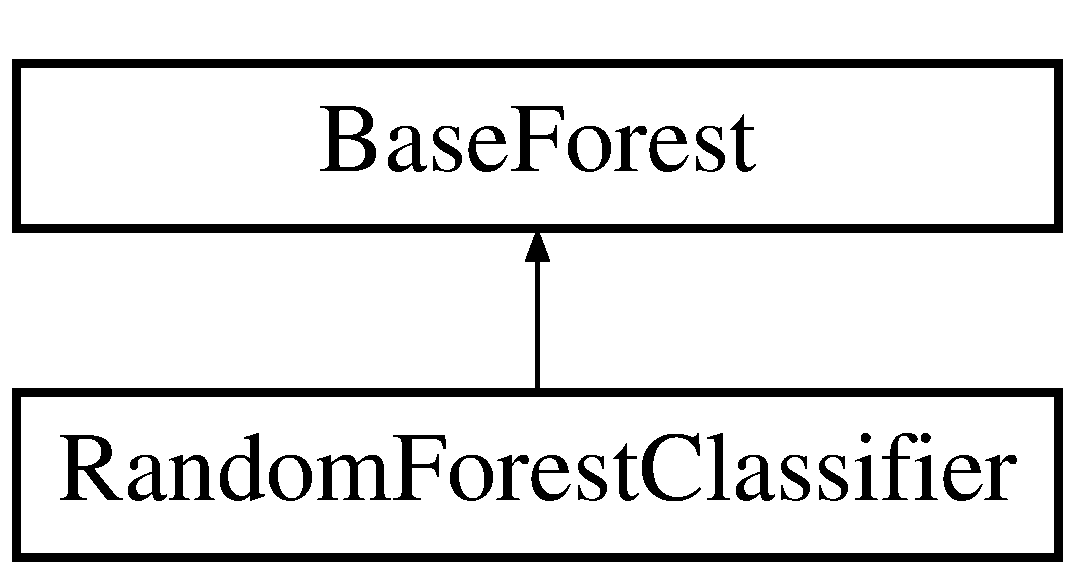
\includegraphics[height=2.000000cm]{class_base_forest}
\end{center}
\end{figure}
\subsection*{Public Member Functions}
\begin{DoxyCompactItemize}
\item 
\hyperlink{class_base_forest_ad32c78f5827091945a82f6b24c1b188e}{Base\+Forest} ()
\item 
\hyperlink{class_base_forest_a21026b45283f5977dcbe9f9cd5bfe4b3}{Base\+Forest} (int \hyperlink{class_base_forest_a2549a0057ec5419fe1de52ef198125ce}{n\+\_\+trees}, int \hyperlink{class_base_forest_a94fe86e1b426d149a11d100921cea3a4}{n\+\_\+threads}=\hyperlink{class_base_forest_a36733c1fadd0daadba8e694ee30fd1b6}{D\+E\+F\+A\+U\+L\+T\+\_\+\+N\+\_\+\+T\+H\+R\+E\+A\+D\+S}, std\+::string \hyperlink{class_base_forest_a5c651ace1f9d5177cdff38a0ae4048f7}{max\+\_\+feature\+\_\+criterion}=\char`\"{}sqrt\char`\"{}, int \hyperlink{class_base_forest_a85cf2e2e202c6e82bf684057181138f6}{max\+\_\+depth}=\hyperlink{class_base_forest_ac6df44eee4d7ee5913ad57d1d6c79692}{D\+E\+F\+A\+U\+L\+T\+\_\+\+M\+A\+X\+\_\+\+D\+E\+P\+T\+H}, int \hyperlink{class_base_forest_a15e0407f3c0fbc4c25e0796c781ff059}{min\+\_\+leaf\+\_\+samples}=\hyperlink{class_base_forest_a3d000d7f9e2410c73b41b70d8e2e58f8}{D\+E\+F\+A\+U\+L\+T\+\_\+\+M\+I\+N\+\_\+\+L\+E\+A\+F\+\_\+\+S\+A\+M\+P\+L\+E\+S})
\item 
\hyperlink{class_base_forest_a39f3ce33df66a2d327395211774bd344}{$\sim$\+Base\+Forest} ()
\end{DoxyCompactItemize}
\subsection*{Protected Attributes}
\begin{DoxyCompactItemize}
\item 
int \hyperlink{class_base_forest_a94fe86e1b426d149a11d100921cea3a4}{n\+\_\+threads}
\item 
int \hyperlink{class_base_forest_a2549a0057ec5419fe1de52ef198125ce}{n\+\_\+trees}
\item 
std\+::string \hyperlink{class_base_forest_a5c651ace1f9d5177cdff38a0ae4048f7}{max\+\_\+feature\+\_\+criterion}
\item 
int \hyperlink{class_base_forest_a07e8b0ed27405f469198f2c4875786c9}{max\+\_\+feature}
\item 
int \hyperlink{class_base_forest_a07e5f38350cc60220dab5661f378b776}{n\+\_\+classes}
\item 
int \hyperlink{class_base_forest_a85cf2e2e202c6e82bf684057181138f6}{max\+\_\+depth}
\item 
int \hyperlink{class_base_forest_a15e0407f3c0fbc4c25e0796c781ff059}{min\+\_\+leaf\+\_\+samples}
\item 
Dataset $\ast$ \hyperlink{class_base_forest_abb0fa17c78f968b583bc15139f409dd5}{ds}
\item 
std\+::vector$<$ Base\+Tree $\ast$ $>$ \hyperlink{class_base_forest_a1a271bf9403c4181aff21e54d1a5e255}{forest}
\end{DoxyCompactItemize}
\subsection*{Static Protected Attributes}
\begin{DoxyCompactItemize}
\item 
static const int \hyperlink{class_base_forest_a36733c1fadd0daadba8e694ee30fd1b6}{D\+E\+F\+A\+U\+L\+T\+\_\+\+N\+\_\+\+T\+H\+R\+E\+A\+D\+S} = 1
\item 
static const int \hyperlink{class_base_forest_a5a697ac9a46154b8f551c012820ffd56}{D\+E\+F\+A\+U\+L\+T\+\_\+\+N\+\_\+\+T\+R\+E\+E\+S} = 10
\item 
static const int \hyperlink{class_base_forest_ac6df44eee4d7ee5913ad57d1d6c79692}{D\+E\+F\+A\+U\+L\+T\+\_\+\+M\+A\+X\+\_\+\+D\+E\+P\+T\+H} = -\/1
\item 
static const int \hyperlink{class_base_forest_a3d000d7f9e2410c73b41b70d8e2e58f8}{D\+E\+F\+A\+U\+L\+T\+\_\+\+M\+I\+N\+\_\+\+L\+E\+A\+F\+\_\+\+S\+A\+M\+P\+L\+E\+S} = 1
\item 
static const std\+::string \hyperlink{class_base_forest_af72e5270729ceae48ca24163a35b46af}{D\+E\+F\+A\+U\+L\+T\+\_\+\+M\+A\+X\+\_\+\+F\+E\+A\+T\+U\+R\+E\+\_\+\+C\+R\+I\+T\+E\+R\+I\+O\+N} = \char`\"{}sqrt\char`\"{}
\end{DoxyCompactItemize}
\subsection*{Private Member Functions}
\begin{DoxyCompactItemize}
\item 
void \hyperlink{class_base_forest_acbd8fb7a63430c5f07633cc5c4e43a3d}{init} (int \hyperlink{class_base_forest_a2549a0057ec5419fe1de52ef198125ce}{n\+\_\+trees}, int \hyperlink{class_base_forest_a94fe86e1b426d149a11d100921cea3a4}{n\+\_\+threads}, std\+::string \hyperlink{class_base_forest_a5c651ace1f9d5177cdff38a0ae4048f7}{max\+\_\+feature\+\_\+criterion}, int \hyperlink{class_base_forest_a85cf2e2e202c6e82bf684057181138f6}{max\+\_\+depth}, int \hyperlink{class_base_forest_a15e0407f3c0fbc4c25e0796c781ff059}{min\+\_\+leaf\+\_\+samples})
\item 
void \hyperlink{class_base_forest_a8d6af13b5f3fbd592d6abe5f6e0e6028}{check\+\_\+param} (int n\+\_\+tree, int \hyperlink{class_base_forest_a94fe86e1b426d149a11d100921cea3a4}{n\+\_\+threads}, std\+::string \hyperlink{class_base_forest_a07e8b0ed27405f469198f2c4875786c9}{max\+\_\+feature}, int \hyperlink{class_base_forest_a85cf2e2e202c6e82bf684057181138f6}{max\+\_\+depth}, int \hyperlink{class_base_forest_a15e0407f3c0fbc4c25e0796c781ff059}{min\+\_\+leaf\+\_\+samples})
\end{DoxyCompactItemize}


\subsection{Constructor \& Destructor Documentation}
\hypertarget{class_base_forest_ad32c78f5827091945a82f6b24c1b188e}{\index{Base\+Forest@{Base\+Forest}!Base\+Forest@{Base\+Forest}}
\index{Base\+Forest@{Base\+Forest}!Base\+Forest@{Base\+Forest}}
\subsubsection[{Base\+Forest}]{\setlength{\rightskip}{0pt plus 5cm}Base\+Forest\+::\+Base\+Forest (
\begin{DoxyParamCaption}
{}
\end{DoxyParamCaption}
)}}\label{class_base_forest_ad32c78f5827091945a82f6b24c1b188e}
\hypertarget{class_base_forest_a21026b45283f5977dcbe9f9cd5bfe4b3}{\index{Base\+Forest@{Base\+Forest}!Base\+Forest@{Base\+Forest}}
\index{Base\+Forest@{Base\+Forest}!Base\+Forest@{Base\+Forest}}
\subsubsection[{Base\+Forest}]{\setlength{\rightskip}{0pt plus 5cm}Base\+Forest\+::\+Base\+Forest (
\begin{DoxyParamCaption}
\item[{int}]{n\+\_\+trees, }
\item[{int}]{n\+\_\+threads = {\ttfamily {\bf D\+E\+F\+A\+U\+L\+T\+\_\+\+N\+\_\+\+T\+H\+R\+E\+A\+D\+S}}, }
\item[{std\+::string}]{max\+\_\+feature\+\_\+criterion = {\ttfamily \char`\"{}sqrt\char`\"{}}, }
\item[{int}]{max\+\_\+depth = {\ttfamily {\bf D\+E\+F\+A\+U\+L\+T\+\_\+\+M\+A\+X\+\_\+\+D\+E\+P\+T\+H}}, }
\item[{int}]{min\+\_\+leaf\+\_\+samples = {\ttfamily {\bf D\+E\+F\+A\+U\+L\+T\+\_\+\+M\+I\+N\+\_\+\+L\+E\+A\+F\+\_\+\+S\+A\+M\+P\+L\+E\+S}}}
\end{DoxyParamCaption}
)}}\label{class_base_forest_a21026b45283f5977dcbe9f9cd5bfe4b3}
\hypertarget{class_base_forest_a39f3ce33df66a2d327395211774bd344}{\index{Base\+Forest@{Base\+Forest}!````~Base\+Forest@{$\sim$\+Base\+Forest}}
\index{````~Base\+Forest@{$\sim$\+Base\+Forest}!Base\+Forest@{Base\+Forest}}
\subsubsection[{$\sim$\+Base\+Forest}]{\setlength{\rightskip}{0pt plus 5cm}Base\+Forest\+::$\sim$\+Base\+Forest (
\begin{DoxyParamCaption}
{}
\end{DoxyParamCaption}
)}}\label{class_base_forest_a39f3ce33df66a2d327395211774bd344}


\subsection{Member Function Documentation}
\hypertarget{class_base_forest_a8d6af13b5f3fbd592d6abe5f6e0e6028}{\index{Base\+Forest@{Base\+Forest}!check\+\_\+param@{check\+\_\+param}}
\index{check\+\_\+param@{check\+\_\+param}!Base\+Forest@{Base\+Forest}}
\subsubsection[{check\+\_\+param}]{\setlength{\rightskip}{0pt plus 5cm}void Base\+Forest\+::check\+\_\+param (
\begin{DoxyParamCaption}
\item[{int}]{n\+\_\+tree, }
\item[{int}]{n\+\_\+threads, }
\item[{std\+::string}]{max\+\_\+feature, }
\item[{int}]{max\+\_\+depth, }
\item[{int}]{min\+\_\+leaf\+\_\+samples}
\end{DoxyParamCaption}
)\hspace{0.3cm}{\ttfamily [private]}}}\label{class_base_forest_a8d6af13b5f3fbd592d6abe5f6e0e6028}
\hypertarget{class_base_forest_acbd8fb7a63430c5f07633cc5c4e43a3d}{\index{Base\+Forest@{Base\+Forest}!init@{init}}
\index{init@{init}!Base\+Forest@{Base\+Forest}}
\subsubsection[{init}]{\setlength{\rightskip}{0pt plus 5cm}void Base\+Forest\+::init (
\begin{DoxyParamCaption}
\item[{int}]{n\+\_\+trees, }
\item[{int}]{n\+\_\+threads, }
\item[{std\+::string}]{max\+\_\+feature\+\_\+criterion, }
\item[{int}]{max\+\_\+depth, }
\item[{int}]{min\+\_\+leaf\+\_\+samples}
\end{DoxyParamCaption}
)\hspace{0.3cm}{\ttfamily [private]}}}\label{class_base_forest_acbd8fb7a63430c5f07633cc5c4e43a3d}


\subsection{Member Data Documentation}
\hypertarget{class_base_forest_ac6df44eee4d7ee5913ad57d1d6c79692}{\index{Base\+Forest@{Base\+Forest}!D\+E\+F\+A\+U\+L\+T\+\_\+\+M\+A\+X\+\_\+\+D\+E\+P\+T\+H@{D\+E\+F\+A\+U\+L\+T\+\_\+\+M\+A\+X\+\_\+\+D\+E\+P\+T\+H}}
\index{D\+E\+F\+A\+U\+L\+T\+\_\+\+M\+A\+X\+\_\+\+D\+E\+P\+T\+H@{D\+E\+F\+A\+U\+L\+T\+\_\+\+M\+A\+X\+\_\+\+D\+E\+P\+T\+H}!Base\+Forest@{Base\+Forest}}
\subsubsection[{D\+E\+F\+A\+U\+L\+T\+\_\+\+M\+A\+X\+\_\+\+D\+E\+P\+T\+H}]{\setlength{\rightskip}{0pt plus 5cm}const int Base\+Forest\+::\+D\+E\+F\+A\+U\+L\+T\+\_\+\+M\+A\+X\+\_\+\+D\+E\+P\+T\+H = -\/1\hspace{0.3cm}{\ttfamily [static]}, {\ttfamily [protected]}}}\label{class_base_forest_ac6df44eee4d7ee5913ad57d1d6c79692}
\hypertarget{class_base_forest_af72e5270729ceae48ca24163a35b46af}{\index{Base\+Forest@{Base\+Forest}!D\+E\+F\+A\+U\+L\+T\+\_\+\+M\+A\+X\+\_\+\+F\+E\+A\+T\+U\+R\+E\+\_\+\+C\+R\+I\+T\+E\+R\+I\+O\+N@{D\+E\+F\+A\+U\+L\+T\+\_\+\+M\+A\+X\+\_\+\+F\+E\+A\+T\+U\+R\+E\+\_\+\+C\+R\+I\+T\+E\+R\+I\+O\+N}}
\index{D\+E\+F\+A\+U\+L\+T\+\_\+\+M\+A\+X\+\_\+\+F\+E\+A\+T\+U\+R\+E\+\_\+\+C\+R\+I\+T\+E\+R\+I\+O\+N@{D\+E\+F\+A\+U\+L\+T\+\_\+\+M\+A\+X\+\_\+\+F\+E\+A\+T\+U\+R\+E\+\_\+\+C\+R\+I\+T\+E\+R\+I\+O\+N}!Base\+Forest@{Base\+Forest}}
\subsubsection[{D\+E\+F\+A\+U\+L\+T\+\_\+\+M\+A\+X\+\_\+\+F\+E\+A\+T\+U\+R\+E\+\_\+\+C\+R\+I\+T\+E\+R\+I\+O\+N}]{\setlength{\rightskip}{0pt plus 5cm}const std\+::string Base\+Forest\+::\+D\+E\+F\+A\+U\+L\+T\+\_\+\+M\+A\+X\+\_\+\+F\+E\+A\+T\+U\+R\+E\+\_\+\+C\+R\+I\+T\+E\+R\+I\+O\+N = \char`\"{}sqrt\char`\"{}\hspace{0.3cm}{\ttfamily [static]}, {\ttfamily [protected]}}}\label{class_base_forest_af72e5270729ceae48ca24163a35b46af}
\hypertarget{class_base_forest_a3d000d7f9e2410c73b41b70d8e2e58f8}{\index{Base\+Forest@{Base\+Forest}!D\+E\+F\+A\+U\+L\+T\+\_\+\+M\+I\+N\+\_\+\+L\+E\+A\+F\+\_\+\+S\+A\+M\+P\+L\+E\+S@{D\+E\+F\+A\+U\+L\+T\+\_\+\+M\+I\+N\+\_\+\+L\+E\+A\+F\+\_\+\+S\+A\+M\+P\+L\+E\+S}}
\index{D\+E\+F\+A\+U\+L\+T\+\_\+\+M\+I\+N\+\_\+\+L\+E\+A\+F\+\_\+\+S\+A\+M\+P\+L\+E\+S@{D\+E\+F\+A\+U\+L\+T\+\_\+\+M\+I\+N\+\_\+\+L\+E\+A\+F\+\_\+\+S\+A\+M\+P\+L\+E\+S}!Base\+Forest@{Base\+Forest}}
\subsubsection[{D\+E\+F\+A\+U\+L\+T\+\_\+\+M\+I\+N\+\_\+\+L\+E\+A\+F\+\_\+\+S\+A\+M\+P\+L\+E\+S}]{\setlength{\rightskip}{0pt plus 5cm}const int Base\+Forest\+::\+D\+E\+F\+A\+U\+L\+T\+\_\+\+M\+I\+N\+\_\+\+L\+E\+A\+F\+\_\+\+S\+A\+M\+P\+L\+E\+S = 1\hspace{0.3cm}{\ttfamily [static]}, {\ttfamily [protected]}}}\label{class_base_forest_a3d000d7f9e2410c73b41b70d8e2e58f8}
\hypertarget{class_base_forest_a36733c1fadd0daadba8e694ee30fd1b6}{\index{Base\+Forest@{Base\+Forest}!D\+E\+F\+A\+U\+L\+T\+\_\+\+N\+\_\+\+T\+H\+R\+E\+A\+D\+S@{D\+E\+F\+A\+U\+L\+T\+\_\+\+N\+\_\+\+T\+H\+R\+E\+A\+D\+S}}
\index{D\+E\+F\+A\+U\+L\+T\+\_\+\+N\+\_\+\+T\+H\+R\+E\+A\+D\+S@{D\+E\+F\+A\+U\+L\+T\+\_\+\+N\+\_\+\+T\+H\+R\+E\+A\+D\+S}!Base\+Forest@{Base\+Forest}}
\subsubsection[{D\+E\+F\+A\+U\+L\+T\+\_\+\+N\+\_\+\+T\+H\+R\+E\+A\+D\+S}]{\setlength{\rightskip}{0pt plus 5cm}const int Base\+Forest\+::\+D\+E\+F\+A\+U\+L\+T\+\_\+\+N\+\_\+\+T\+H\+R\+E\+A\+D\+S = 1\hspace{0.3cm}{\ttfamily [static]}, {\ttfamily [protected]}}}\label{class_base_forest_a36733c1fadd0daadba8e694ee30fd1b6}
\hypertarget{class_base_forest_a5a697ac9a46154b8f551c012820ffd56}{\index{Base\+Forest@{Base\+Forest}!D\+E\+F\+A\+U\+L\+T\+\_\+\+N\+\_\+\+T\+R\+E\+E\+S@{D\+E\+F\+A\+U\+L\+T\+\_\+\+N\+\_\+\+T\+R\+E\+E\+S}}
\index{D\+E\+F\+A\+U\+L\+T\+\_\+\+N\+\_\+\+T\+R\+E\+E\+S@{D\+E\+F\+A\+U\+L\+T\+\_\+\+N\+\_\+\+T\+R\+E\+E\+S}!Base\+Forest@{Base\+Forest}}
\subsubsection[{D\+E\+F\+A\+U\+L\+T\+\_\+\+N\+\_\+\+T\+R\+E\+E\+S}]{\setlength{\rightskip}{0pt plus 5cm}const int Base\+Forest\+::\+D\+E\+F\+A\+U\+L\+T\+\_\+\+N\+\_\+\+T\+R\+E\+E\+S = 10\hspace{0.3cm}{\ttfamily [static]}, {\ttfamily [protected]}}}\label{class_base_forest_a5a697ac9a46154b8f551c012820ffd56}
\hypertarget{class_base_forest_abb0fa17c78f968b583bc15139f409dd5}{\index{Base\+Forest@{Base\+Forest}!ds@{ds}}
\index{ds@{ds}!Base\+Forest@{Base\+Forest}}
\subsubsection[{ds}]{\setlength{\rightskip}{0pt plus 5cm}Dataset$\ast$ Base\+Forest\+::ds\hspace{0.3cm}{\ttfamily [protected]}}}\label{class_base_forest_abb0fa17c78f968b583bc15139f409dd5}
\hypertarget{class_base_forest_a1a271bf9403c4181aff21e54d1a5e255}{\index{Base\+Forest@{Base\+Forest}!forest@{forest}}
\index{forest@{forest}!Base\+Forest@{Base\+Forest}}
\subsubsection[{forest}]{\setlength{\rightskip}{0pt plus 5cm}std\+::vector$<$Base\+Tree$\ast$$>$ Base\+Forest\+::forest\hspace{0.3cm}{\ttfamily [protected]}}}\label{class_base_forest_a1a271bf9403c4181aff21e54d1a5e255}
\hypertarget{class_base_forest_a85cf2e2e202c6e82bf684057181138f6}{\index{Base\+Forest@{Base\+Forest}!max\+\_\+depth@{max\+\_\+depth}}
\index{max\+\_\+depth@{max\+\_\+depth}!Base\+Forest@{Base\+Forest}}
\subsubsection[{max\+\_\+depth}]{\setlength{\rightskip}{0pt plus 5cm}int Base\+Forest\+::max\+\_\+depth\hspace{0.3cm}{\ttfamily [protected]}}}\label{class_base_forest_a85cf2e2e202c6e82bf684057181138f6}
\hypertarget{class_base_forest_a07e8b0ed27405f469198f2c4875786c9}{\index{Base\+Forest@{Base\+Forest}!max\+\_\+feature@{max\+\_\+feature}}
\index{max\+\_\+feature@{max\+\_\+feature}!Base\+Forest@{Base\+Forest}}
\subsubsection[{max\+\_\+feature}]{\setlength{\rightskip}{0pt plus 5cm}int Base\+Forest\+::max\+\_\+feature\hspace{0.3cm}{\ttfamily [protected]}}}\label{class_base_forest_a07e8b0ed27405f469198f2c4875786c9}
\hypertarget{class_base_forest_a5c651ace1f9d5177cdff38a0ae4048f7}{\index{Base\+Forest@{Base\+Forest}!max\+\_\+feature\+\_\+criterion@{max\+\_\+feature\+\_\+criterion}}
\index{max\+\_\+feature\+\_\+criterion@{max\+\_\+feature\+\_\+criterion}!Base\+Forest@{Base\+Forest}}
\subsubsection[{max\+\_\+feature\+\_\+criterion}]{\setlength{\rightskip}{0pt plus 5cm}std\+::string Base\+Forest\+::max\+\_\+feature\+\_\+criterion\hspace{0.3cm}{\ttfamily [protected]}}}\label{class_base_forest_a5c651ace1f9d5177cdff38a0ae4048f7}
\hypertarget{class_base_forest_a15e0407f3c0fbc4c25e0796c781ff059}{\index{Base\+Forest@{Base\+Forest}!min\+\_\+leaf\+\_\+samples@{min\+\_\+leaf\+\_\+samples}}
\index{min\+\_\+leaf\+\_\+samples@{min\+\_\+leaf\+\_\+samples}!Base\+Forest@{Base\+Forest}}
\subsubsection[{min\+\_\+leaf\+\_\+samples}]{\setlength{\rightskip}{0pt plus 5cm}int Base\+Forest\+::min\+\_\+leaf\+\_\+samples\hspace{0.3cm}{\ttfamily [protected]}}}\label{class_base_forest_a15e0407f3c0fbc4c25e0796c781ff059}
\hypertarget{class_base_forest_a07e5f38350cc60220dab5661f378b776}{\index{Base\+Forest@{Base\+Forest}!n\+\_\+classes@{n\+\_\+classes}}
\index{n\+\_\+classes@{n\+\_\+classes}!Base\+Forest@{Base\+Forest}}
\subsubsection[{n\+\_\+classes}]{\setlength{\rightskip}{0pt plus 5cm}int Base\+Forest\+::n\+\_\+classes\hspace{0.3cm}{\ttfamily [protected]}}}\label{class_base_forest_a07e5f38350cc60220dab5661f378b776}
\hypertarget{class_base_forest_a94fe86e1b426d149a11d100921cea3a4}{\index{Base\+Forest@{Base\+Forest}!n\+\_\+threads@{n\+\_\+threads}}
\index{n\+\_\+threads@{n\+\_\+threads}!Base\+Forest@{Base\+Forest}}
\subsubsection[{n\+\_\+threads}]{\setlength{\rightskip}{0pt plus 5cm}int Base\+Forest\+::n\+\_\+threads\hspace{0.3cm}{\ttfamily [protected]}}}\label{class_base_forest_a94fe86e1b426d149a11d100921cea3a4}
\hypertarget{class_base_forest_a2549a0057ec5419fe1de52ef198125ce}{\index{Base\+Forest@{Base\+Forest}!n\+\_\+trees@{n\+\_\+trees}}
\index{n\+\_\+trees@{n\+\_\+trees}!Base\+Forest@{Base\+Forest}}
\subsubsection[{n\+\_\+trees}]{\setlength{\rightskip}{0pt plus 5cm}int Base\+Forest\+::n\+\_\+trees\hspace{0.3cm}{\ttfamily [protected]}}}\label{class_base_forest_a2549a0057ec5419fe1de52ef198125ce}


The documentation for this class was generated from the following files\+:\begin{DoxyCompactItemize}
\item 
\hyperlink{forest_8h}{forest.\+h}\item 
\hyperlink{forest_8cpp}{forest.\+cpp}\end{DoxyCompactItemize}

\hypertarget{classbatch__node}{\section{batch\+\_\+node Class Reference}
\label{classbatch__node}\index{batch\+\_\+node@{batch\+\_\+node}}
}


Specify for batch tree algorithm (e.\+g. decision tree)  




{\ttfamily \#include $<$tree.\+h$>$}

Inheritance diagram for batch\+\_\+node\+:\begin{figure}[H]
\begin{center}
\leavevmode
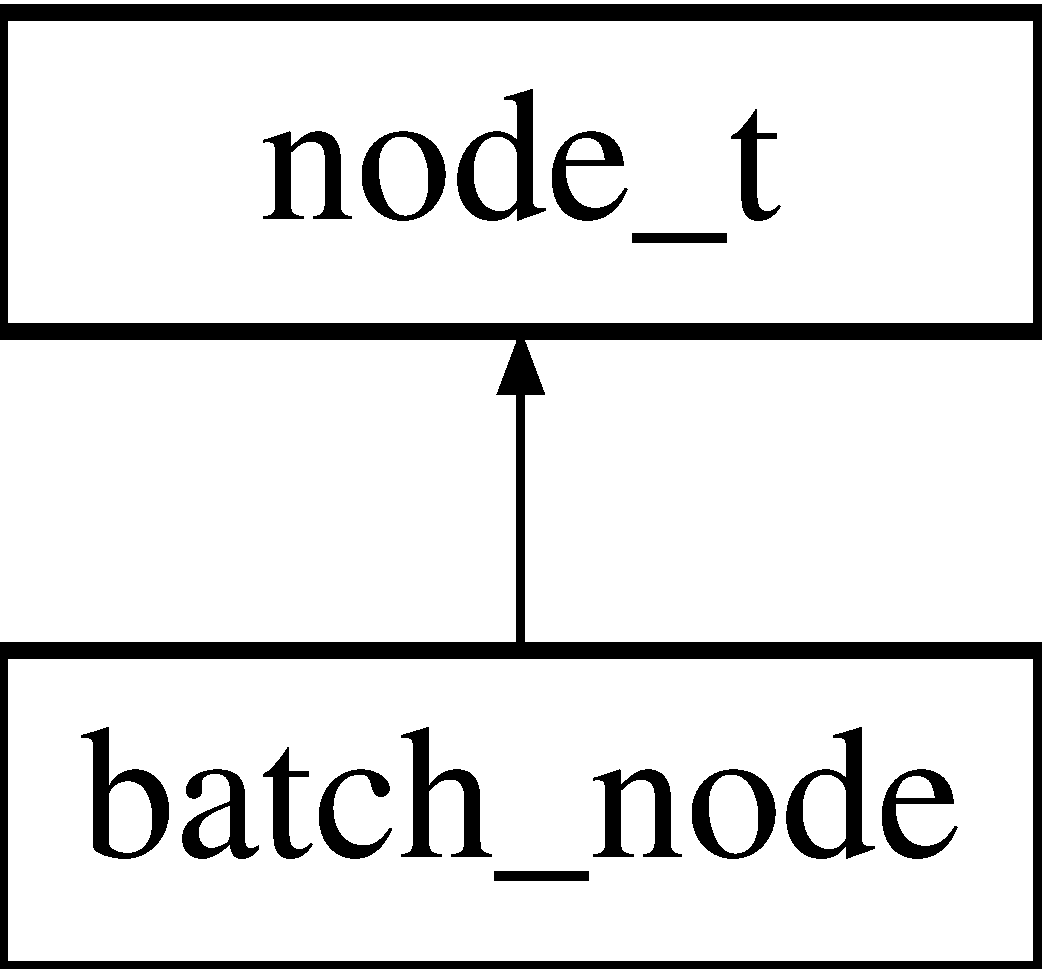
\includegraphics[height=2.000000cm]{classbatch__node}
\end{center}
\end{figure}
\subsection*{Public Member Functions}
\begin{DoxyCompactItemize}
\item 
\hyperlink{classbatch__node_ab5d0146c446c311a10c382234f4f4aa0}{batch\+\_\+node} (int \hyperlink{classnode_a8c4864582cb3fe15e84e7908d0965150}{n\+\_\+classes})
\end{DoxyCompactItemize}
\subsection*{Additional Inherited Members}


\subsection{Detailed Description}
Specify for batch tree algorithm (e.\+g. decision tree) 

\subsection{Constructor \& Destructor Documentation}
\hypertarget{classbatch__node_ab5d0146c446c311a10c382234f4f4aa0}{\index{batch\+\_\+node@{batch\+\_\+node}!batch\+\_\+node@{batch\+\_\+node}}
\index{batch\+\_\+node@{batch\+\_\+node}!batch\+\_\+node@{batch\+\_\+node}}
\subsubsection[{batch\+\_\+node}]{\setlength{\rightskip}{0pt plus 5cm}batch\+\_\+node\+::batch\+\_\+node (
\begin{DoxyParamCaption}
\item[{int}]{n\+\_\+classes}
\end{DoxyParamCaption}
)}}\label{classbatch__node_ab5d0146c446c311a10c382234f4f4aa0}


The documentation for this class was generated from the following files\+:\begin{DoxyCompactItemize}
\item 
\hyperlink{tree_8h}{tree.\+h}\item 
\hyperlink{tree_8cpp}{tree.\+cpp}\end{DoxyCompactItemize}

\hypertarget{classbest__splitter}{\section{best\+\_\+splitter Class Reference}
\label{classbest__splitter}\index{best\+\_\+splitter@{best\+\_\+splitter}}
}


{\ttfamily \#include $<$tree.\+h$>$}

Inheritance diagram for best\+\_\+splitter\+:\begin{figure}[H]
\begin{center}
\leavevmode
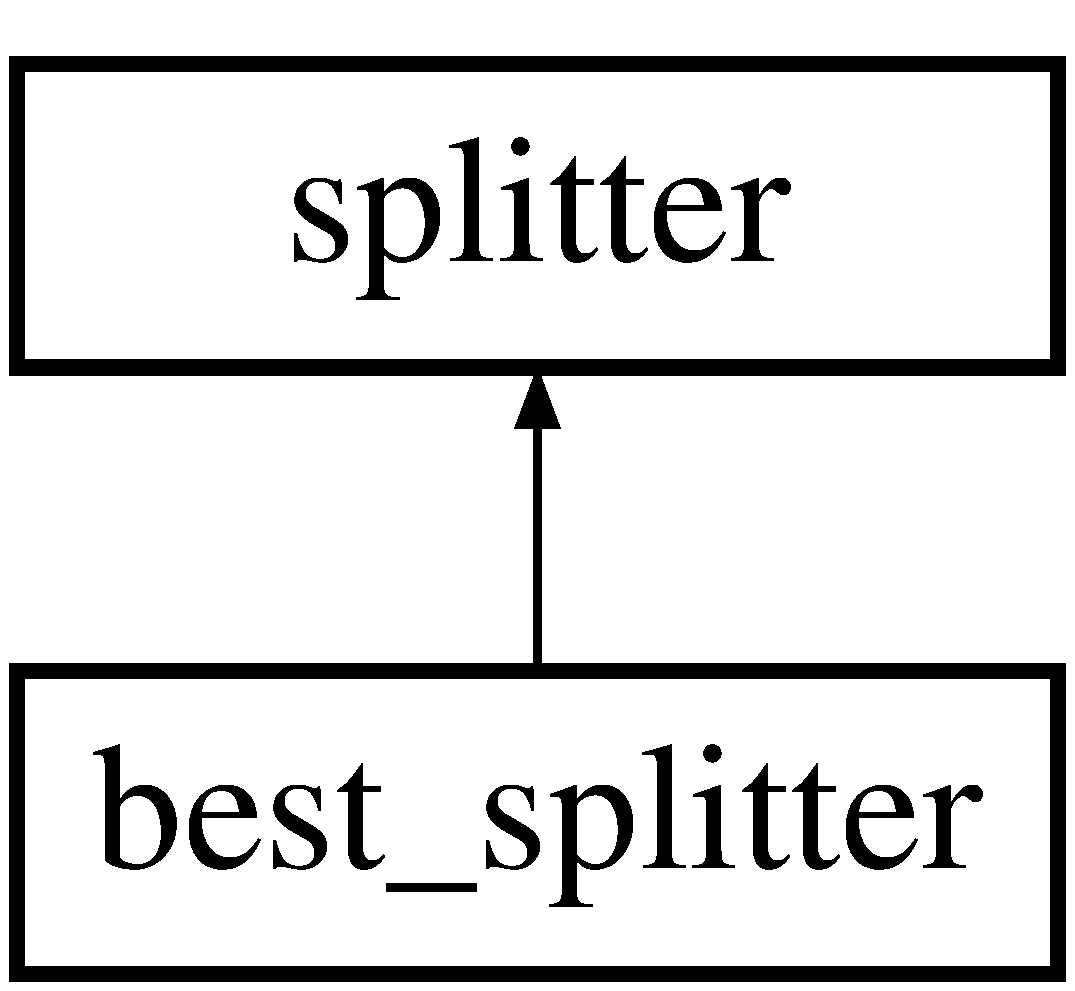
\includegraphics[height=2.000000cm]{classbest__splitter}
\end{center}
\end{figure}
\subsection*{Public Member Functions}
\begin{DoxyCompactItemize}
\item 
void \hyperlink{classbest__splitter_ae090eae85590c1184bb172c7bcd56751}{split} (\hyperlink{classtree}{tree} $\ast$\&t, \hyperlink{classnode}{node} $\ast$\&root, \hyperlink{classdataset}{dataset} $\ast$\&d, \hyperlink{classcriterion}{criterion} $\ast$\&cr)
\item 
void \hyperlink{classbest__splitter_a681ad1823db5207f3a5a6acd5c09b354}{update} (int \hyperlink{classsplitter_ad093754efc111ae9dcb00e844b91e979}{fea\+\_\+id}, float \hyperlink{classsplitter_af40121f8411ad94f3f1968b1d50905ed}{threshold}, float $\ast$\&left, \hyperlink{classnode}{node} $\ast$\&nd, \hyperlink{classcriterion}{criterion} $\ast$\&cr)
\end{DoxyCompactItemize}
\subsection*{Additional Inherited Members}


\subsection{Member Function Documentation}
\hypertarget{classbest__splitter_ae090eae85590c1184bb172c7bcd56751}{\index{best\+\_\+splitter@{best\+\_\+splitter}!split@{split}}
\index{split@{split}!best\+\_\+splitter@{best\+\_\+splitter}}
\subsubsection[{split}]{\setlength{\rightskip}{0pt plus 5cm}void best\+\_\+splitter\+::split (
\begin{DoxyParamCaption}
\item[{{\bf tree} $\ast$\&}]{t, }
\item[{{\bf node} $\ast$\&}]{root, }
\item[{{\bf dataset} $\ast$\&}]{d, }
\item[{{\bf criterion} $\ast$\&}]{cr}
\end{DoxyParamCaption}
)\hspace{0.3cm}{\ttfamily [virtual]}}}\label{classbest__splitter_ae090eae85590c1184bb172c7bcd56751}


Implements \hyperlink{classsplitter_a5795eaf65be951d241ad697e20fb2120}{splitter}.

\hypertarget{classbest__splitter_a681ad1823db5207f3a5a6acd5c09b354}{\index{best\+\_\+splitter@{best\+\_\+splitter}!update@{update}}
\index{update@{update}!best\+\_\+splitter@{best\+\_\+splitter}}
\subsubsection[{update}]{\setlength{\rightskip}{0pt plus 5cm}void best\+\_\+splitter\+::update (
\begin{DoxyParamCaption}
\item[{int}]{fea\+\_\+id, }
\item[{float}]{threshold, }
\item[{float $\ast$\&}]{left, }
\item[{{\bf node} $\ast$\&}]{nd, }
\item[{{\bf criterion} $\ast$\&}]{cr}
\end{DoxyParamCaption}
)\hspace{0.3cm}{\ttfamily [virtual]}}}\label{classbest__splitter_a681ad1823db5207f3a5a6acd5c09b354}


Implements \hyperlink{classsplitter_ab2ea956cc1a10ebb39422fa5ac450af2}{splitter}.



The documentation for this class was generated from the following files\+:\begin{DoxyCompactItemize}
\item 
\hyperlink{tree_8h}{tree.\+h}\item 
\hyperlink{tree_8cpp}{tree.\+cpp}\end{DoxyCompactItemize}

\hypertarget{classcriterion}{\section{criterion Class Reference}
\label{classcriterion}\index{criterion@{criterion}}
}


Heuristic measure.  




{\ttfamily \#include $<$tree.\+h$>$}

Inheritance diagram for criterion\+:\begin{figure}[H]
\begin{center}
\leavevmode
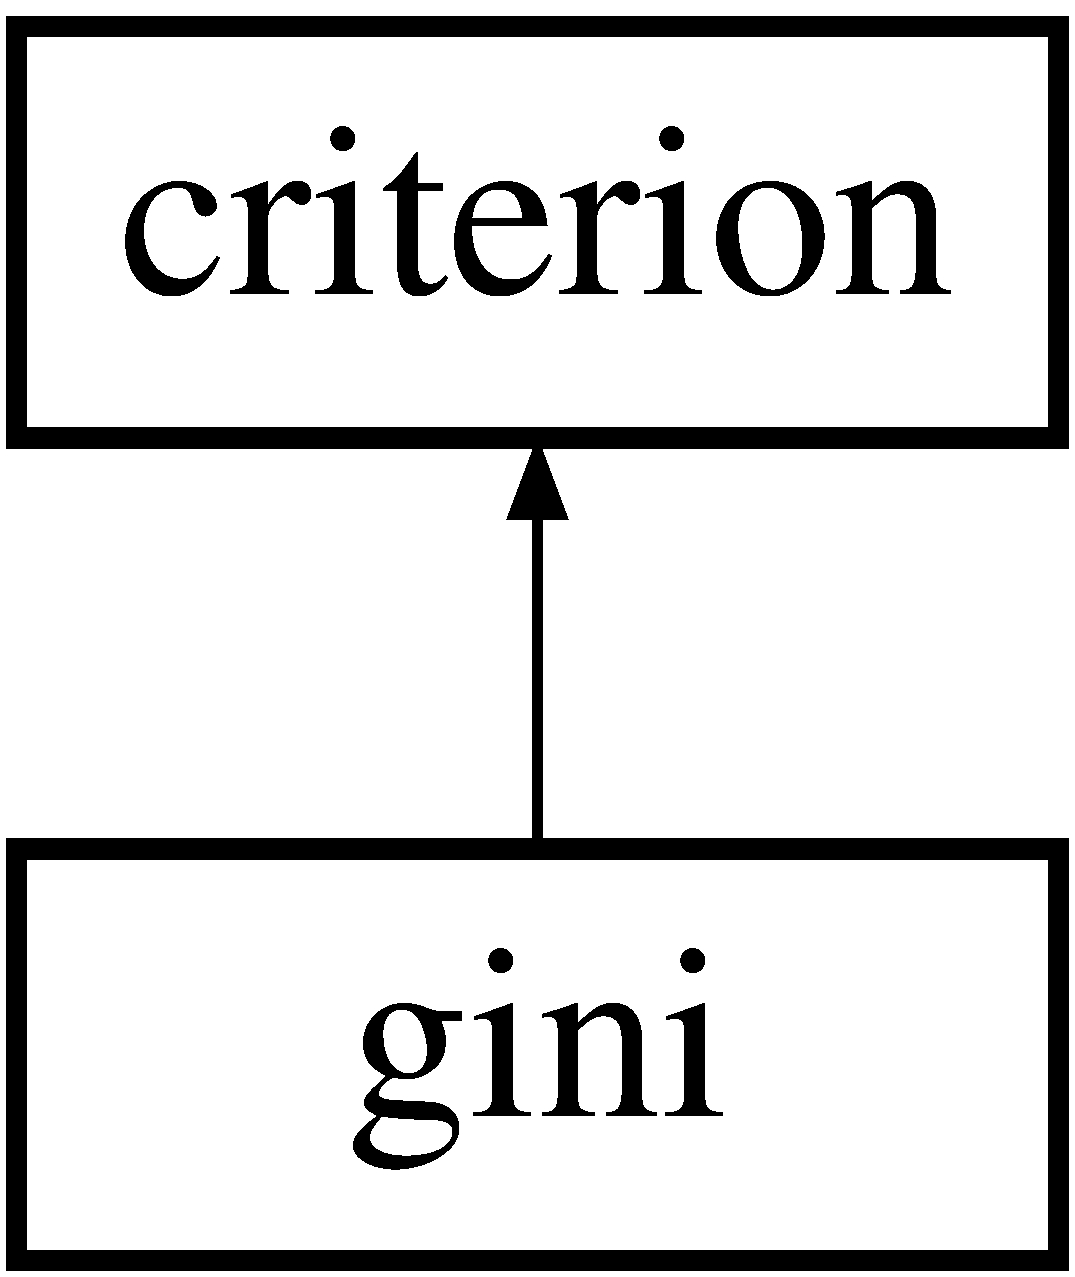
\includegraphics[height=2.000000cm]{classcriterion}
\end{center}
\end{figure}
\subsection*{Public Member Functions}
\begin{DoxyCompactItemize}
\item 
\hyperlink{classcriterion_a5047629e45833624bc6955cc0dd106b8}{criterion} ()
\begin{DoxyCompactList}\small\item\em Constructor (need to call {\ttfamily set\+\_\+current} function manually) \end{DoxyCompactList}\item 
\hyperlink{classcriterion_acf80c0b2acf9fb6f2b8369868cafdbff}{criterion} (float $\ast$\&frequency, int n\+\_\+classes)
\begin{DoxyCompactList}\small\item\em Constructor. \end{DoxyCompactList}\item 
virtual \hyperlink{classcriterion_aab29d10fad28cb5eeb5d3e212ecb5656}{$\sim$criterion} ()
\begin{DoxyCompactList}\small\item\em $\sim$criterion destructor \end{DoxyCompactList}\item 
void \hyperlink{classcriterion_a043c2105b2cfc256cb530c55b65156f2}{set\+\_\+current} (float $\ast$\&frequency, int n\+\_\+classes)
\begin{DoxyCompactList}\small\item\em Intialize the current node information because compute {\ttfamily gain} need the current node's heuristic measure (e.\+g. information gain, gini index) \end{DoxyCompactList}\item 
float \hyperlink{classcriterion_a8d42878c94bae5a72475b568bcbbddfa}{gain} (float $\ast$\&left\+\_\+frequency, float $\ast$\&right\+\_\+frequency, int n\+\_\+classes)
\begin{DoxyCompactList}\small\item\em Heuristic measure value gain after the split. \end{DoxyCompactList}\item 
virtual float \hyperlink{classcriterion_a1fbda0723578acd5ac612248a54ba71d}{measure} (float $\ast$\&frequency, int n\+\_\+classes)=0
\begin{DoxyCompactList}\small\item\em Heuristic measure value. \end{DoxyCompactList}\end{DoxyCompactItemize}
\subsection*{Protected Attributes}
\begin{DoxyCompactItemize}
\item 
float \hyperlink{classcriterion_ac226599a3e6e160614d3698193053368}{tot\+\_\+frequency}
\item 
float \hyperlink{classcriterion_af8e6efc16000b83cffb9e0864bf68561}{cur\+\_\+measure}
\item 
float \hyperlink{classcriterion_aa89bec3e37cd874b3590887038712c54}{cur\+\_\+tot}
\item 
bool \hyperlink{classcriterion_a5f3c4708d9e6a9120ec8b8d98c73ff47}{is\+\_\+init}
\end{DoxyCompactItemize}


\subsection{Detailed Description}
Heuristic measure. 

\subsection{Constructor \& Destructor Documentation}
\hypertarget{classcriterion_a5047629e45833624bc6955cc0dd106b8}{\index{criterion@{criterion}!criterion@{criterion}}
\index{criterion@{criterion}!criterion@{criterion}}
\subsubsection[{criterion}]{\setlength{\rightskip}{0pt plus 5cm}criterion\+::criterion (
\begin{DoxyParamCaption}
{}
\end{DoxyParamCaption}
)}}\label{classcriterion_a5047629e45833624bc6955cc0dd106b8}


Constructor (need to call {\ttfamily set\+\_\+current} function manually) 

has set the current node measure \hypertarget{classcriterion_acf80c0b2acf9fb6f2b8369868cafdbff}{\index{criterion@{criterion}!criterion@{criterion}}
\index{criterion@{criterion}!criterion@{criterion}}
\subsubsection[{criterion}]{\setlength{\rightskip}{0pt plus 5cm}criterion\+::criterion (
\begin{DoxyParamCaption}
\item[{float $\ast$\&}]{frequency, }
\item[{int}]{n\+\_\+classes}
\end{DoxyParamCaption}
)}}\label{classcriterion_acf80c0b2acf9fb6f2b8369868cafdbff}


Constructor. 


\begin{DoxyParams}{Parameters}
{\em frequency} & frequency for each class in parent node (sum of each example's weight) \\
\hline
{\em n\+\_\+classes} & number of different classes \\
\hline
\end{DoxyParams}
\hypertarget{classcriterion_aab29d10fad28cb5eeb5d3e212ecb5656}{\index{criterion@{criterion}!````~criterion@{$\sim$criterion}}
\index{````~criterion@{$\sim$criterion}!criterion@{criterion}}
\subsubsection[{$\sim$criterion}]{\setlength{\rightskip}{0pt plus 5cm}criterion\+::$\sim$criterion (
\begin{DoxyParamCaption}
{}
\end{DoxyParamCaption}
)\hspace{0.3cm}{\ttfamily [virtual]}}}\label{classcriterion_aab29d10fad28cb5eeb5d3e212ecb5656}


$\sim$criterion destructor 



\subsection{Member Function Documentation}
\hypertarget{classcriterion_a8d42878c94bae5a72475b568bcbbddfa}{\index{criterion@{criterion}!gain@{gain}}
\index{gain@{gain}!criterion@{criterion}}
\subsubsection[{gain}]{\setlength{\rightskip}{0pt plus 5cm}float criterion\+::gain (
\begin{DoxyParamCaption}
\item[{float $\ast$\&}]{left\+\_\+frequency, }
\item[{float $\ast$\&}]{right\+\_\+frequency, }
\item[{int}]{n\+\_\+classes}
\end{DoxyParamCaption}
)}}\label{classcriterion_a8d42878c94bae5a72475b568bcbbddfa}


Heuristic measure value gain after the split. 


\begin{DoxyParams}{Parameters}
{\em left\+\_\+frequency} & left node's frequency (frequency definition can be found in the constructor function) \\
\hline
{\em right\+\_\+frequency} & right node's frequency (frequency definition can be found in the constructor function) \\
\hline
{\em n\+\_\+classes} & number of different classes\\
\hline
\end{DoxyParams}
\begin{DoxyReturn}{Returns}
heurist measure value gain 
\end{DoxyReturn}
\hypertarget{classcriterion_a1fbda0723578acd5ac612248a54ba71d}{\index{criterion@{criterion}!measure@{measure}}
\index{measure@{measure}!criterion@{criterion}}
\subsubsection[{measure}]{\setlength{\rightskip}{0pt plus 5cm}virtual float criterion\+::measure (
\begin{DoxyParamCaption}
\item[{float $\ast$\&}]{frequency, }
\item[{int}]{n\+\_\+classes}
\end{DoxyParamCaption}
)\hspace{0.3cm}{\ttfamily [pure virtual]}}}\label{classcriterion_a1fbda0723578acd5ac612248a54ba71d}


Heuristic measure value. 


\begin{DoxyParams}{Parameters}
{\em frequency} & frequency for each class in the node \\
\hline
{\em n\+\_\+classes} & number of different classes\\
\hline
\end{DoxyParams}
\begin{DoxyReturn}{Returns}
heuristic measure value 
\end{DoxyReturn}


Implemented in \hyperlink{classgini_a5f232df1155fe182eee9b26cde0e8339}{gini}.

\hypertarget{classcriterion_a043c2105b2cfc256cb530c55b65156f2}{\index{criterion@{criterion}!set\+\_\+current@{set\+\_\+current}}
\index{set\+\_\+current@{set\+\_\+current}!criterion@{criterion}}
\subsubsection[{set\+\_\+current}]{\setlength{\rightskip}{0pt plus 5cm}void criterion\+::set\+\_\+current (
\begin{DoxyParamCaption}
\item[{float $\ast$\&}]{frequency, }
\item[{int}]{n\+\_\+classes}
\end{DoxyParamCaption}
)}}\label{classcriterion_a043c2105b2cfc256cb530c55b65156f2}


Intialize the current node information because compute {\ttfamily gain} need the current node's heuristic measure (e.\+g. information gain, gini index) 


\begin{DoxyParams}{Parameters}
{\em frequency} & frequency for each class in parent node (sum of each example's weight) \\
\hline
{\em n\+\_\+classes} & number of different classes \\
\hline
\end{DoxyParams}


\subsection{Member Data Documentation}
\hypertarget{classcriterion_af8e6efc16000b83cffb9e0864bf68561}{\index{criterion@{criterion}!cur\+\_\+measure@{cur\+\_\+measure}}
\index{cur\+\_\+measure@{cur\+\_\+measure}!criterion@{criterion}}
\subsubsection[{cur\+\_\+measure}]{\setlength{\rightskip}{0pt plus 5cm}float criterion\+::cur\+\_\+measure\hspace{0.3cm}{\ttfamily [protected]}}}\label{classcriterion_af8e6efc16000b83cffb9e0864bf68561}
temporary variable store {\ttfamily tot\+\_\+frequency} after calling {\ttfamily measure} function \hypertarget{classcriterion_aa89bec3e37cd874b3590887038712c54}{\index{criterion@{criterion}!cur\+\_\+tot@{cur\+\_\+tot}}
\index{cur\+\_\+tot@{cur\+\_\+tot}!criterion@{criterion}}
\subsubsection[{cur\+\_\+tot}]{\setlength{\rightskip}{0pt plus 5cm}float criterion\+::cur\+\_\+tot\hspace{0.3cm}{\ttfamily [protected]}}}\label{classcriterion_aa89bec3e37cd874b3590887038712c54}
current node heuristic measure value \hypertarget{classcriterion_a5f3c4708d9e6a9120ec8b8d98c73ff47}{\index{criterion@{criterion}!is\+\_\+init@{is\+\_\+init}}
\index{is\+\_\+init@{is\+\_\+init}!criterion@{criterion}}
\subsubsection[{is\+\_\+init}]{\setlength{\rightskip}{0pt plus 5cm}bool criterion\+::is\+\_\+init\hspace{0.3cm}{\ttfamily [protected]}}}\label{classcriterion_a5f3c4708d9e6a9120ec8b8d98c73ff47}
current node total frequency \hypertarget{classcriterion_ac226599a3e6e160614d3698193053368}{\index{criterion@{criterion}!tot\+\_\+frequency@{tot\+\_\+frequency}}
\index{tot\+\_\+frequency@{tot\+\_\+frequency}!criterion@{criterion}}
\subsubsection[{tot\+\_\+frequency}]{\setlength{\rightskip}{0pt plus 5cm}float criterion\+::tot\+\_\+frequency\hspace{0.3cm}{\ttfamily [protected]}}}\label{classcriterion_ac226599a3e6e160614d3698193053368}


The documentation for this class was generated from the following files\+:\begin{DoxyCompactItemize}
\item 
include/\hyperlink{tree_8h}{tree.\+h}\item 
src/\hyperlink{tree_8cpp}{tree.\+cpp}\end{DoxyCompactItemize}

\hypertarget{classdata__reader}{\section{data\+\_\+reader Class Reference}
\label{classdata__reader}\index{data\+\_\+reader@{data\+\_\+reader}}
}


{\ttfamily \#include $<$dataset.\+h$>$}

\subsection*{Public Member Functions}
\begin{DoxyCompactItemize}
\item 
\hyperlink{classdata__reader_abffe82f72b9ccfff618e3c3b0fff774e}{data\+\_\+reader} (const std\+::string \&filename, int \hyperlink{classdata__reader_ab77f1bebd79be09216119e127b463434}{n\+\_\+features}, const \hyperlink{dataset_8h_a87dfee910993320c6720931fb701cc41}{learn\+\_\+mode} \hyperlink{classdata__reader_a4132a7abcf03cca64e2eb204e70fffd3}{mode})
\begin{DoxyCompactList}\small\item\em \hyperlink{classdata__reader}{data\+\_\+reader} constructor \end{DoxyCompactList}\item 
\hyperlink{classdata__reader_afae224dd7295e44e0b4efefe3cb5efdf}{$\sim$data\+\_\+reader} ()
\begin{DoxyCompactList}\small\item\em $\sim$data\+\_\+reader destructor \end{DoxyCompactList}\item 
\hyperlink{classexample__t}{example\+\_\+t} $\ast$ \hyperlink{classdata__reader_ae2ff1315d03cb16c55861a77f08cd87b}{read\+\_\+an\+\_\+example} ()
\begin{DoxyCompactList}\small\item\em read\+\_\+an\+\_\+example read an example \end{DoxyCompactList}\item 
std\+::vector$<$ \hyperlink{classexample__t}{example\+\_\+t} $\ast$ $>$ \hyperlink{classdata__reader_a2fa952493f9f348861c6ba7a0c65a578}{read\+\_\+examples} ()
\begin{DoxyCompactList}\small\item\em read\+\_\+examples read all the example \end{DoxyCompactList}\end{DoxyCompactItemize}
\subsection*{Private Attributes}
\begin{DoxyCompactItemize}
\item 
int \hyperlink{classdata__reader_ab77f1bebd79be09216119e127b463434}{n\+\_\+features}
\item 
std\+::ifstream \hyperlink{classdata__reader_a1a39328bde93e7f132a1ca7eb6642311}{ifs}
\item 
\hyperlink{dataset_8h_a87dfee910993320c6720931fb701cc41}{learn\+\_\+mode} \hyperlink{classdata__reader_a4132a7abcf03cca64e2eb204e70fffd3}{mode}
\end{DoxyCompactItemize}


\subsection{Constructor \& Destructor Documentation}
\hypertarget{classdata__reader_abffe82f72b9ccfff618e3c3b0fff774e}{\index{data\+\_\+reader@{data\+\_\+reader}!data\+\_\+reader@{data\+\_\+reader}}
\index{data\+\_\+reader@{data\+\_\+reader}!data\+\_\+reader@{data\+\_\+reader}}
\subsubsection[{data\+\_\+reader}]{\setlength{\rightskip}{0pt plus 5cm}data\+\_\+reader\+::data\+\_\+reader (
\begin{DoxyParamCaption}
\item[{const std\+::string \&}]{filename, }
\item[{int}]{n\+\_\+features, }
\item[{const {\bf learn\+\_\+mode}}]{mode}
\end{DoxyParamCaption}
)}}\label{classdata__reader_abffe82f72b9ccfff618e3c3b0fff774e}


\hyperlink{classdata__reader}{data\+\_\+reader} constructor 

learn mode 
\begin{DoxyParams}{Parameters}
{\em n\+\_\+features} & number of features \\
\hline
{\em mode} & train or predict \\
\hline
\end{DoxyParams}
\hypertarget{classdata__reader_afae224dd7295e44e0b4efefe3cb5efdf}{\index{data\+\_\+reader@{data\+\_\+reader}!````~data\+\_\+reader@{$\sim$data\+\_\+reader}}
\index{````~data\+\_\+reader@{$\sim$data\+\_\+reader}!data\+\_\+reader@{data\+\_\+reader}}
\subsubsection[{$\sim$data\+\_\+reader}]{\setlength{\rightskip}{0pt plus 5cm}data\+\_\+reader\+::$\sim$data\+\_\+reader (
\begin{DoxyParamCaption}
{}
\end{DoxyParamCaption}
)}}\label{classdata__reader_afae224dd7295e44e0b4efefe3cb5efdf}


$\sim$data\+\_\+reader destructor 



\subsection{Member Function Documentation}
\hypertarget{classdata__reader_ae2ff1315d03cb16c55861a77f08cd87b}{\index{data\+\_\+reader@{data\+\_\+reader}!read\+\_\+an\+\_\+example@{read\+\_\+an\+\_\+example}}
\index{read\+\_\+an\+\_\+example@{read\+\_\+an\+\_\+example}!data\+\_\+reader@{data\+\_\+reader}}
\subsubsection[{read\+\_\+an\+\_\+example}]{\setlength{\rightskip}{0pt plus 5cm}{\bf example\+\_\+t} $\ast$ data\+\_\+reader\+::read\+\_\+an\+\_\+example (
\begin{DoxyParamCaption}
{}
\end{DoxyParamCaption}
)}}\label{classdata__reader_ae2ff1315d03cb16c55861a77f08cd87b}


read\+\_\+an\+\_\+example read an example 


\begin{DoxyParams}{Parameters}
{\em ifs} & input file stream to read example\\
\hline
\end{DoxyParams}
\begin{DoxyReturn}{Returns}
a single example's features 
\end{DoxyReturn}
\hypertarget{classdata__reader_a2fa952493f9f348861c6ba7a0c65a578}{\index{data\+\_\+reader@{data\+\_\+reader}!read\+\_\+examples@{read\+\_\+examples}}
\index{read\+\_\+examples@{read\+\_\+examples}!data\+\_\+reader@{data\+\_\+reader}}
\subsubsection[{read\+\_\+examples}]{\setlength{\rightskip}{0pt plus 5cm}std\+::vector$<$ {\bf example\+\_\+t} $\ast$ $>$ data\+\_\+reader\+::read\+\_\+examples (
\begin{DoxyParamCaption}
{}
\end{DoxyParamCaption}
)}}\label{classdata__reader_a2fa952493f9f348861c6ba7a0c65a578}


read\+\_\+examples read all the example 


\begin{DoxyParams}{Parameters}
{\em filename} & \\
\hline
\end{DoxyParams}
\begin{DoxyReturn}{Returns}
a vector contains all examples' features 
\end{DoxyReturn}


\subsection{Member Data Documentation}
\hypertarget{classdata__reader_a1a39328bde93e7f132a1ca7eb6642311}{\index{data\+\_\+reader@{data\+\_\+reader}!ifs@{ifs}}
\index{ifs@{ifs}!data\+\_\+reader@{data\+\_\+reader}}
\subsubsection[{ifs}]{\setlength{\rightskip}{0pt plus 5cm}std\+::ifstream data\+\_\+reader\+::ifs\hspace{0.3cm}{\ttfamily [private]}}}\label{classdata__reader_a1a39328bde93e7f132a1ca7eb6642311}
number of features in the input file \hypertarget{classdata__reader_a4132a7abcf03cca64e2eb204e70fffd3}{\index{data\+\_\+reader@{data\+\_\+reader}!mode@{mode}}
\index{mode@{mode}!data\+\_\+reader@{data\+\_\+reader}}
\subsubsection[{mode}]{\setlength{\rightskip}{0pt plus 5cm}{\bf learn\+\_\+mode} data\+\_\+reader\+::mode\hspace{0.3cm}{\ttfamily [private]}}}\label{classdata__reader_a4132a7abcf03cca64e2eb204e70fffd3}
input file stream related to the input file \hypertarget{classdata__reader_ab77f1bebd79be09216119e127b463434}{\index{data\+\_\+reader@{data\+\_\+reader}!n\+\_\+features@{n\+\_\+features}}
\index{n\+\_\+features@{n\+\_\+features}!data\+\_\+reader@{data\+\_\+reader}}
\subsubsection[{n\+\_\+features}]{\setlength{\rightskip}{0pt plus 5cm}int data\+\_\+reader\+::n\+\_\+features\hspace{0.3cm}{\ttfamily [private]}}}\label{classdata__reader_ab77f1bebd79be09216119e127b463434}


The documentation for this class was generated from the following files\+:\begin{DoxyCompactItemize}
\item 
include/\hyperlink{dataset_8h}{dataset.\+h}\item 
src/\hyperlink{dataset_8cpp}{dataset.\+cpp}\end{DoxyCompactItemize}

\hypertarget{classdataset}{\section{dataset Class Reference}
\label{classdataset}\index{dataset@{dataset}}
}


{\ttfamily \#include $<$dataset.\+h$>$}

\subsection*{Public Member Functions}
\begin{DoxyCompactItemize}
\item 
\hyperlink{classdataset_a7cb166d5282c5d6e66242764f9148a94}{dataset} ()
\begin{DoxyCompactList}\small\item\em dataset constructor \end{DoxyCompactList}\item 
\hyperlink{classdataset_acfaf71f71b7ddb95a77431e3663aa4a1}{dataset} (int \hyperlink{classdataset_aa33a77fd21cbed4019bfb5ed82e30c6b}{n\+\_\+classes}, int \hyperlink{classdataset_a5469ac8f1b5d64d836821e5056599b54}{n\+\_\+features}, float $\ast$\hyperlink{classdataset_ac6690ca832182b7cfa64da93a6ccd6ab}{weight})
\begin{DoxyCompactList}\small\item\em dataset constructor \end{DoxyCompactList}\item 
\hyperlink{classdataset_a770010cb1e1da07bea9ed9dd665a6d65}{$\sim$dataset} ()
\begin{DoxyCompactList}\small\item\em $\sim$dataset destructor \end{DoxyCompactList}\item 
void \hyperlink{classdataset_a53d6ced8ba17a1ff4771ab53ffda85ef}{init} (int \hyperlink{classdataset_aa33a77fd21cbed4019bfb5ed82e30c6b}{n\+\_\+classes}, int \hyperlink{classdataset_a5469ac8f1b5d64d836821e5056599b54}{n\+\_\+features}, float $\ast$\hyperlink{classdataset_ac6690ca832182b7cfa64da93a6ccd6ab}{weight})
\begin{DoxyCompactList}\small\item\em init \end{DoxyCompactList}\item 
void \hyperlink{classdataset_a0bf2fba4da731ca757f0cb2bd95fe172}{load\+\_\+data} (const std\+::string \&filename, const \hyperlink{dataset_8h_a87dfee910993320c6720931fb701cc41}{learn\+\_\+mode} \hyperlink{classdataset_a47d44ca9cd02a4dc98ff80e0616a5aa9}{mode})
\begin{DoxyCompactList}\small\item\em load\+\_\+data generate the dataset from input file \end{DoxyCompactList}\item 
void \hyperlink{classdataset_aeab51be94fab1f62e901555c82a016ae}{load\+\_\+data\+\_\+meta} (const std\+::string \&filename)
\begin{DoxyCompactList}\small\item\em load\+\_\+data\+\_\+meta \end{DoxyCompactList}\item 
void \hyperlink{classdataset_aeca876714406b8e391ab8cdeb31c9f3f}{debug} ()
\begin{DoxyCompactList}\small\item\em debug print some information for debugging \end{DoxyCompactList}\item 
int \hyperlink{classdataset_a35b101f3d8aecd5d87820982718f1534}{get\+\_\+nclasses} ()
\item 
int \hyperlink{classdataset_acd3afb9c245b9e11a6ed53ea293257a9}{get\+\_\+nexamples} ()
\item 
int \hyperlink{classdataset_a956095a460089726c8f39b3de8d4173d}{get\+\_\+nfeatures} ()
\end{DoxyCompactItemize}
\subsection*{Public Attributes}
\begin{DoxyCompactItemize}
\item 
\hyperlink{structev__pair__t}{ev\+\_\+pair\+\_\+t} $\ast$$\ast$ \hyperlink{classdataset_af7977ae76ce8f573f349e63f6500a8f8}{x}
\item 
int $\ast$ \hyperlink{classdataset_acc18732fc7fbc0fcdebffac620646eb9}{size}
\item 
\hyperlink{dataset_8h_a0f180d1f400ce1743488c55eb82a0a49}{target\+\_\+t} $\ast$ \hyperlink{classdataset_a146d2d2d0eaadeb342e76b9bb1004881}{y}
\item 
float $\ast$ \hyperlink{classdataset_ac6690ca832182b7cfa64da93a6ccd6ab}{weight}
\item 
bool $\ast$ \hyperlink{classdataset_ab856d84d4bced1ccde106badfab229d8}{is\+\_\+cate}
\end{DoxyCompactItemize}
\subsection*{Private Member Functions}
\begin{DoxyCompactItemize}
\item 
void \hyperlink{classdataset_a0a5e275e95d935b8d864b35e2dfd3933}{isort} (\hyperlink{structev__pair__t}{ev\+\_\+pair\+\_\+t} $\ast$a, int $\ast$f, int n)
\begin{DoxyCompactList}\small\item\em isort code comes from {\ttfamily fest package} \href{http://lowrank.net/nikos/fest/}{\tt http\+://lowrank.\+net/nikos/fest/} \end{DoxyCompactList}\item 
void \hyperlink{classdataset_a8008be7b546cc9ec90005557ad0ee289}{qsortlazy} (\hyperlink{structev__pair__t}{ev\+\_\+pair\+\_\+t} $\ast$a, int $\ast$f, int l, int u)
\begin{DoxyCompactList}\small\item\em qsortlazy code comes from {\ttfamily fest package} \href{http://lowrank.net/nikos/fest/}{\tt http\+://lowrank.\+net/nikos/fest/} \end{DoxyCompactList}\item 
void \hyperlink{classdataset_a8d1c382f82b2365674a87de56dae9ac1}{sort} (\hyperlink{structev__pair__t}{ev\+\_\+pair\+\_\+t} $\ast$a, int $\ast$f, int len)
\begin{DoxyCompactList}\small\item\em sort code comes from {\ttfamily fest package} \href{http://lowrank.net/nikos/fest/}{\tt http\+://lowrank.\+net/nikos/fest/} \end{DoxyCompactList}\end{DoxyCompactItemize}
\subsection*{Private Attributes}
\begin{DoxyCompactItemize}
\item 
int \hyperlink{classdataset_aa33a77fd21cbed4019bfb5ed82e30c6b}{n\+\_\+classes}
\item 
int \hyperlink{classdataset_ad7186a7fc9e74633c3b3fcddcf241ad4}{n\+\_\+examples}
\item 
int \hyperlink{classdataset_a5469ac8f1b5d64d836821e5056599b54}{n\+\_\+features}
\item 
bool \hyperlink{classdataset_ab5381427833c91ee35913ca1c1d4e73b}{is\+\_\+init}
\item 
\hyperlink{dataset_8h_a87dfee910993320c6720931fb701cc41}{learn\+\_\+mode} \hyperlink{classdataset_a47d44ca9cd02a4dc98ff80e0616a5aa9}{mode}
\end{DoxyCompactItemize}


\subsection{Constructor \& Destructor Documentation}
\hypertarget{classdataset_a7cb166d5282c5d6e66242764f9148a94}{\index{dataset@{dataset}!dataset@{dataset}}
\index{dataset@{dataset}!dataset@{dataset}}
\subsubsection[{dataset}]{\setlength{\rightskip}{0pt plus 5cm}dataset\+::dataset (
\begin{DoxyParamCaption}
{}
\end{DoxyParamCaption}
)}}\label{classdataset_a7cb166d5282c5d6e66242764f9148a94}


dataset constructor 

is the ith attribute categorical \hypertarget{classdataset_acfaf71f71b7ddb95a77431e3663aa4a1}{\index{dataset@{dataset}!dataset@{dataset}}
\index{dataset@{dataset}!dataset@{dataset}}
\subsubsection[{dataset}]{\setlength{\rightskip}{0pt plus 5cm}dataset\+::dataset (
\begin{DoxyParamCaption}
\item[{int}]{n\+\_\+classes, }
\item[{int}]{n\+\_\+features, }
\item[{float $\ast$}]{weight}
\end{DoxyParamCaption}
)}}\label{classdataset_acfaf71f71b7ddb95a77431e3663aa4a1}


dataset constructor 


\begin{DoxyParams}{Parameters}
{\em n\+\_\+classes} & number of classes in the training set \\
\hline
{\em n\+\_\+features} & number of features \\
\hline
{\em weight} & weight for each class \\
\hline
\end{DoxyParams}
\hypertarget{classdataset_a770010cb1e1da07bea9ed9dd665a6d65}{\index{dataset@{dataset}!````~dataset@{$\sim$dataset}}
\index{````~dataset@{$\sim$dataset}!dataset@{dataset}}
\subsubsection[{$\sim$dataset}]{\setlength{\rightskip}{0pt plus 5cm}dataset\+::$\sim$dataset (
\begin{DoxyParamCaption}
{}
\end{DoxyParamCaption}
)}}\label{classdataset_a770010cb1e1da07bea9ed9dd665a6d65}


$\sim$dataset destructor 



\subsection{Member Function Documentation}
\hypertarget{classdataset_aeca876714406b8e391ab8cdeb31c9f3f}{\index{dataset@{dataset}!debug@{debug}}
\index{debug@{debug}!dataset@{dataset}}
\subsubsection[{debug}]{\setlength{\rightskip}{0pt plus 5cm}void dataset\+::debug (
\begin{DoxyParamCaption}
{}
\end{DoxyParamCaption}
)}}\label{classdataset_aeca876714406b8e391ab8cdeb31c9f3f}


debug print some information for debugging 

\hypertarget{classdataset_a35b101f3d8aecd5d87820982718f1534}{\index{dataset@{dataset}!get\+\_\+nclasses@{get\+\_\+nclasses}}
\index{get\+\_\+nclasses@{get\+\_\+nclasses}!dataset@{dataset}}
\subsubsection[{get\+\_\+nclasses}]{\setlength{\rightskip}{0pt plus 5cm}int dataset\+::get\+\_\+nclasses (
\begin{DoxyParamCaption}
{}
\end{DoxyParamCaption}
)}}\label{classdataset_a35b101f3d8aecd5d87820982718f1534}
\hypertarget{classdataset_acd3afb9c245b9e11a6ed53ea293257a9}{\index{dataset@{dataset}!get\+\_\+nexamples@{get\+\_\+nexamples}}
\index{get\+\_\+nexamples@{get\+\_\+nexamples}!dataset@{dataset}}
\subsubsection[{get\+\_\+nexamples}]{\setlength{\rightskip}{0pt plus 5cm}int dataset\+::get\+\_\+nexamples (
\begin{DoxyParamCaption}
{}
\end{DoxyParamCaption}
)}}\label{classdataset_acd3afb9c245b9e11a6ed53ea293257a9}
\hypertarget{classdataset_a956095a460089726c8f39b3de8d4173d}{\index{dataset@{dataset}!get\+\_\+nfeatures@{get\+\_\+nfeatures}}
\index{get\+\_\+nfeatures@{get\+\_\+nfeatures}!dataset@{dataset}}
\subsubsection[{get\+\_\+nfeatures}]{\setlength{\rightskip}{0pt plus 5cm}int dataset\+::get\+\_\+nfeatures (
\begin{DoxyParamCaption}
{}
\end{DoxyParamCaption}
)}}\label{classdataset_a956095a460089726c8f39b3de8d4173d}
\hypertarget{classdataset_a53d6ced8ba17a1ff4771ab53ffda85ef}{\index{dataset@{dataset}!init@{init}}
\index{init@{init}!dataset@{dataset}}
\subsubsection[{init}]{\setlength{\rightskip}{0pt plus 5cm}void dataset\+::init (
\begin{DoxyParamCaption}
\item[{int}]{n\+\_\+classes, }
\item[{int}]{n\+\_\+features, }
\item[{float $\ast$}]{weight}
\end{DoxyParamCaption}
)}}\label{classdataset_a53d6ced8ba17a1ff4771ab53ffda85ef}


init 


\begin{DoxyParams}{Parameters}
{\em n\+\_\+classes} & number of classes in the training set \\
\hline
{\em n\+\_\+features} & number of features \\
\hline
{\em weight} & weight for each class \\
\hline
\end{DoxyParams}
\hypertarget{classdataset_a0a5e275e95d935b8d864b35e2dfd3933}{\index{dataset@{dataset}!isort@{isort}}
\index{isort@{isort}!dataset@{dataset}}
\subsubsection[{isort}]{\setlength{\rightskip}{0pt plus 5cm}void dataset\+::isort (
\begin{DoxyParamCaption}
\item[{{\bf ev\+\_\+pair\+\_\+t} $\ast$}]{a, }
\item[{int $\ast$}]{f, }
\item[{int}]{n}
\end{DoxyParamCaption}
)\hspace{0.3cm}{\ttfamily [private]}}}\label{classdataset_a0a5e275e95d935b8d864b35e2dfd3933}


isort code comes from {\ttfamily fest package} \href{http://lowrank.net/nikos/fest/}{\tt http\+://lowrank.\+net/nikos/fest/} 

learn mode 
\begin{DoxyParams}{Parameters}
{\em a} & example\+\_\+id-\/feature\+\_\+value pair array \\
\hline
{\em f} & corresponding feature\+\_\+id in array {\ttfamily a} \\
\hline
{\em n} & array length \\
\hline
\end{DoxyParams}
\hypertarget{classdataset_a0bf2fba4da731ca757f0cb2bd95fe172}{\index{dataset@{dataset}!load\+\_\+data@{load\+\_\+data}}
\index{load\+\_\+data@{load\+\_\+data}!dataset@{dataset}}
\subsubsection[{load\+\_\+data}]{\setlength{\rightskip}{0pt plus 5cm}void dataset\+::load\+\_\+data (
\begin{DoxyParamCaption}
\item[{const std\+::string \&}]{filename, }
\item[{const {\bf learn\+\_\+mode}}]{mode}
\end{DoxyParamCaption}
)}}\label{classdataset_a0bf2fba4da731ca757f0cb2bd95fe172}


load\+\_\+data generate the dataset from input file 


\begin{DoxyParams}{Parameters}
{\em filename} & input file name \\
\hline
{\em mode} & {\ttfamily T\+R\+A\+I\+N} or {\ttfamily P\+R\+E\+D\+I\+C\+T} \\
\hline
\end{DoxyParams}
\hypertarget{classdataset_aeab51be94fab1f62e901555c82a016ae}{\index{dataset@{dataset}!load\+\_\+data\+\_\+meta@{load\+\_\+data\+\_\+meta}}
\index{load\+\_\+data\+\_\+meta@{load\+\_\+data\+\_\+meta}!dataset@{dataset}}
\subsubsection[{load\+\_\+data\+\_\+meta}]{\setlength{\rightskip}{0pt plus 5cm}void dataset\+::load\+\_\+data\+\_\+meta (
\begin{DoxyParamCaption}
\item[{const std\+::string \&}]{filename}
\end{DoxyParamCaption}
)}}\label{classdataset_aeab51be94fab1f62e901555c82a016ae}


load\+\_\+data\+\_\+meta 


\begin{DoxyParams}{Parameters}
{\em filename} & \\
\hline
\end{DoxyParams}
\hypertarget{classdataset_a8008be7b546cc9ec90005557ad0ee289}{\index{dataset@{dataset}!qsortlazy@{qsortlazy}}
\index{qsortlazy@{qsortlazy}!dataset@{dataset}}
\subsubsection[{qsortlazy}]{\setlength{\rightskip}{0pt plus 5cm}void dataset\+::qsortlazy (
\begin{DoxyParamCaption}
\item[{{\bf ev\+\_\+pair\+\_\+t} $\ast$}]{a, }
\item[{int $\ast$}]{f, }
\item[{int}]{l, }
\item[{int}]{u}
\end{DoxyParamCaption}
)\hspace{0.3cm}{\ttfamily [private]}}}\label{classdataset_a8008be7b546cc9ec90005557ad0ee289}


qsortlazy code comes from {\ttfamily fest package} \href{http://lowrank.net/nikos/fest/}{\tt http\+://lowrank.\+net/nikos/fest/} 


\begin{DoxyParams}{Parameters}
{\em a} & example\+\_\+id-\/feature\+\_\+value pair array \\
\hline
{\em f} & corresponding feature\+\_\+id in array {\ttfamily a} \\
\hline
{\em l} & begin index in array \\
\hline
{\em u} & end index in array \\
\hline
\end{DoxyParams}
\hypertarget{classdataset_a8d1c382f82b2365674a87de56dae9ac1}{\index{dataset@{dataset}!sort@{sort}}
\index{sort@{sort}!dataset@{dataset}}
\subsubsection[{sort}]{\setlength{\rightskip}{0pt plus 5cm}void dataset\+::sort (
\begin{DoxyParamCaption}
\item[{{\bf ev\+\_\+pair\+\_\+t} $\ast$}]{a, }
\item[{int $\ast$}]{f, }
\item[{int}]{len}
\end{DoxyParamCaption}
)\hspace{0.3cm}{\ttfamily [private]}}}\label{classdataset_a8d1c382f82b2365674a87de56dae9ac1}


sort code comes from {\ttfamily fest package} \href{http://lowrank.net/nikos/fest/}{\tt http\+://lowrank.\+net/nikos/fest/} 


\begin{DoxyParams}{Parameters}
{\em a} & example\+\_\+id-\/feature\+\_\+value pair array \\
\hline
{\em f} & corresponding feature\+\_\+id in array {\ttfamily a} \\
\hline
{\em len} & array length \\
\hline
\end{DoxyParams}


\subsection{Member Data Documentation}
\hypertarget{classdataset_ab856d84d4bced1ccde106badfab229d8}{\index{dataset@{dataset}!is\+\_\+cate@{is\+\_\+cate}}
\index{is\+\_\+cate@{is\+\_\+cate}!dataset@{dataset}}
\subsubsection[{is\+\_\+cate}]{\setlength{\rightskip}{0pt plus 5cm}bool$\ast$ dataset\+::is\+\_\+cate}}\label{classdataset_ab856d84d4bced1ccde106badfab229d8}
weight for each class \hypertarget{classdataset_ab5381427833c91ee35913ca1c1d4e73b}{\index{dataset@{dataset}!is\+\_\+init@{is\+\_\+init}}
\index{is\+\_\+init@{is\+\_\+init}!dataset@{dataset}}
\subsubsection[{is\+\_\+init}]{\setlength{\rightskip}{0pt plus 5cm}bool dataset\+::is\+\_\+init\hspace{0.3cm}{\ttfamily [private]}}}\label{classdataset_ab5381427833c91ee35913ca1c1d4e73b}
number of attributes \hypertarget{classdataset_a47d44ca9cd02a4dc98ff80e0616a5aa9}{\index{dataset@{dataset}!mode@{mode}}
\index{mode@{mode}!dataset@{dataset}}
\subsubsection[{mode}]{\setlength{\rightskip}{0pt plus 5cm}{\bf learn\+\_\+mode} dataset\+::mode\hspace{0.3cm}{\ttfamily [private]}}}\label{classdataset_a47d44ca9cd02a4dc98ff80e0616a5aa9}
boolean variable to indicate whether dataset has been initialized \hypertarget{classdataset_aa33a77fd21cbed4019bfb5ed82e30c6b}{\index{dataset@{dataset}!n\+\_\+classes@{n\+\_\+classes}}
\index{n\+\_\+classes@{n\+\_\+classes}!dataset@{dataset}}
\subsubsection[{n\+\_\+classes}]{\setlength{\rightskip}{0pt plus 5cm}int dataset\+::n\+\_\+classes\hspace{0.3cm}{\ttfamily [private]}}}\label{classdataset_aa33a77fd21cbed4019bfb5ed82e30c6b}
\hypertarget{classdataset_ad7186a7fc9e74633c3b3fcddcf241ad4}{\index{dataset@{dataset}!n\+\_\+examples@{n\+\_\+examples}}
\index{n\+\_\+examples@{n\+\_\+examples}!dataset@{dataset}}
\subsubsection[{n\+\_\+examples}]{\setlength{\rightskip}{0pt plus 5cm}int dataset\+::n\+\_\+examples\hspace{0.3cm}{\ttfamily [private]}}}\label{classdataset_ad7186a7fc9e74633c3b3fcddcf241ad4}
number of classes \hypertarget{classdataset_a5469ac8f1b5d64d836821e5056599b54}{\index{dataset@{dataset}!n\+\_\+features@{n\+\_\+features}}
\index{n\+\_\+features@{n\+\_\+features}!dataset@{dataset}}
\subsubsection[{n\+\_\+features}]{\setlength{\rightskip}{0pt plus 5cm}int dataset\+::n\+\_\+features\hspace{0.3cm}{\ttfamily [private]}}}\label{classdataset_a5469ac8f1b5d64d836821e5056599b54}
number of examples \hypertarget{classdataset_acc18732fc7fbc0fcdebffac620646eb9}{\index{dataset@{dataset}!size@{size}}
\index{size@{size}!dataset@{dataset}}
\subsubsection[{size}]{\setlength{\rightskip}{0pt plus 5cm}int$\ast$ dataset\+::size}}\label{classdataset_acc18732fc7fbc0fcdebffac620646eb9}
each row is an attribute \hypertarget{classdataset_ac6690ca832182b7cfa64da93a6ccd6ab}{\index{dataset@{dataset}!weight@{weight}}
\index{weight@{weight}!dataset@{dataset}}
\subsubsection[{weight}]{\setlength{\rightskip}{0pt plus 5cm}float$\ast$ dataset\+::weight}}\label{classdataset_ac6690ca832182b7cfa64da93a6ccd6ab}
label for each example \hypertarget{classdataset_af7977ae76ce8f573f349e63f6500a8f8}{\index{dataset@{dataset}!x@{x}}
\index{x@{x}!dataset@{dataset}}
\subsubsection[{x}]{\setlength{\rightskip}{0pt plus 5cm}{\bf ev\+\_\+pair\+\_\+t}$\ast$$\ast$ dataset\+::x}}\label{classdataset_af7977ae76ce8f573f349e63f6500a8f8}
\hypertarget{classdataset_a146d2d2d0eaadeb342e76b9bb1004881}{\index{dataset@{dataset}!y@{y}}
\index{y@{y}!dataset@{dataset}}
\subsubsection[{y}]{\setlength{\rightskip}{0pt plus 5cm}{\bf target\+\_\+t}$\ast$ dataset\+::y}}\label{classdataset_a146d2d2d0eaadeb342e76b9bb1004881}
number of examples with non-\/zero feature values for each attribute 

The documentation for this class was generated from the following files\+:\begin{DoxyCompactItemize}
\item 
\hyperlink{dataset_8h}{dataset.\+h}\item 
\hyperlink{dataset_8cpp}{dataset.\+cpp}\end{DoxyCompactItemize}

\hypertarget{classdecision__tree}{\section{decision\+\_\+tree Class Reference}
\label{classdecision__tree}\index{decision\+\_\+tree@{decision\+\_\+tree}}
}


{\ttfamily \#include $<$tree.\+h$>$}

Inheritance diagram for decision\+\_\+tree\+:\begin{figure}[H]
\begin{center}
\leavevmode
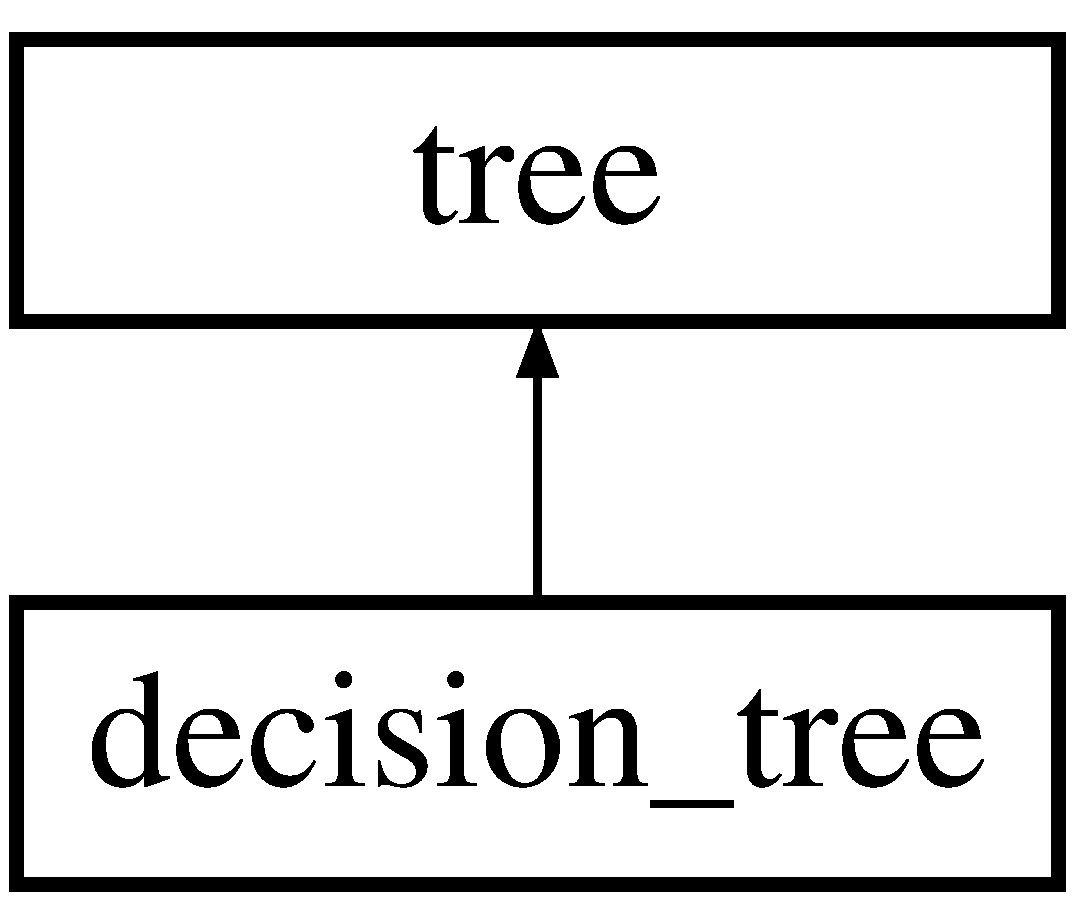
\includegraphics[height=2.000000cm]{classdecision__tree}
\end{center}
\end{figure}
\subsection*{Public Member Functions}
\begin{DoxyCompactItemize}
\item 
void \hyperlink{classdecision__tree_ad3286ad0d5361f3f19ddac966477b14a}{build} (\hyperlink{classdataset}{dataset} $\ast$\&d)
\end{DoxyCompactItemize}
\subsection*{Private Member Functions}
\begin{DoxyCompactItemize}
\item 
void \hyperlink{classdecision__tree_affee9d32ce17c6102083d809da55a847}{build\+\_\+rec} (\hyperlink{classnode}{node} $\ast$\&\hyperlink{classtree_ad397d4906e47149b98f769b3e81473ee}{root}, \hyperlink{classdataset}{dataset} $\ast$\&d, int depth)
\end{DoxyCompactItemize}
\subsection*{Additional Inherited Members}


\subsection{Member Function Documentation}
\hypertarget{classdecision__tree_ad3286ad0d5361f3f19ddac966477b14a}{\index{decision\+\_\+tree@{decision\+\_\+tree}!build@{build}}
\index{build@{build}!decision\+\_\+tree@{decision\+\_\+tree}}
\subsubsection[{build}]{\setlength{\rightskip}{0pt plus 5cm}void decision\+\_\+tree\+::build (
\begin{DoxyParamCaption}
\item[{{\bf dataset} $\ast$\&}]{d}
\end{DoxyParamCaption}
)}}\label{classdecision__tree_ad3286ad0d5361f3f19ddac966477b14a}
\hypertarget{classdecision__tree_affee9d32ce17c6102083d809da55a847}{\index{decision\+\_\+tree@{decision\+\_\+tree}!build\+\_\+rec@{build\+\_\+rec}}
\index{build\+\_\+rec@{build\+\_\+rec}!decision\+\_\+tree@{decision\+\_\+tree}}
\subsubsection[{build\+\_\+rec}]{\setlength{\rightskip}{0pt plus 5cm}void decision\+\_\+tree\+::build\+\_\+rec (
\begin{DoxyParamCaption}
\item[{{\bf node} $\ast$\&}]{root, }
\item[{{\bf dataset} $\ast$\&}]{d, }
\item[{int}]{depth}
\end{DoxyParamCaption}
)\hspace{0.3cm}{\ttfamily [private]}}}\label{classdecision__tree_affee9d32ce17c6102083d809da55a847}


The documentation for this class was generated from the following files\+:\begin{DoxyCompactItemize}
\item 
\hyperlink{tree_8h}{tree.\+h}\item 
\hyperlink{tree_8cpp}{tree.\+cpp}\end{DoxyCompactItemize}

\hypertarget{structev__pair__t}{\section{ev\+\_\+pair\+\_\+t Struct Reference}
\label{structev__pair__t}\index{ev\+\_\+pair\+\_\+t@{ev\+\_\+pair\+\_\+t}}
}


{\ttfamily \#include $<$dataset.\+h$>$}

\subsection*{Public Member Functions}
\begin{DoxyCompactItemize}
\item 
void \hyperlink{structev__pair__t_a394c42bf616c580994570d49d98e09ca}{set} (int \hyperlink{structev__pair__t_aed493fca94855b5ba8081d4e1a7b28f1}{ex\+\_\+id}, \hyperlink{dataset_8h_ac2e4791c62a663377be91b0922cede72}{feature\+\_\+t} \hyperlink{structev__pair__t_ab029b4bacf7dc6db2fee53091f5f8063}{fea\+\_\+value})
\end{DoxyCompactItemize}
\subsection*{Public Attributes}
\begin{DoxyCompactItemize}
\item 
int \hyperlink{structev__pair__t_aed493fca94855b5ba8081d4e1a7b28f1}{ex\+\_\+id}
\item 
\hyperlink{dataset_8h_ac2e4791c62a663377be91b0922cede72}{feature\+\_\+t} \hyperlink{structev__pair__t_ab029b4bacf7dc6db2fee53091f5f8063}{fea\+\_\+value}
\end{DoxyCompactItemize}


\subsection{Detailed Description}
{\ttfamily train} mode or {\ttfamily predict} mode 

\subsection{Member Function Documentation}
\hypertarget{structev__pair__t_a394c42bf616c580994570d49d98e09ca}{\index{ev\+\_\+pair\+\_\+t@{ev\+\_\+pair\+\_\+t}!set@{set}}
\index{set@{set}!ev\+\_\+pair\+\_\+t@{ev\+\_\+pair\+\_\+t}}
\subsubsection[{set}]{\setlength{\rightskip}{0pt plus 5cm}void ev\+\_\+pair\+\_\+t\+::set (
\begin{DoxyParamCaption}
\item[{int}]{ex\+\_\+id, }
\item[{{\bf feature\+\_\+t}}]{fea\+\_\+value}
\end{DoxyParamCaption}
)\hspace{0.3cm}{\ttfamily [inline]}}}\label{structev__pair__t_a394c42bf616c580994570d49d98e09ca}
feature value 

\subsection{Member Data Documentation}
\hypertarget{structev__pair__t_aed493fca94855b5ba8081d4e1a7b28f1}{\index{ev\+\_\+pair\+\_\+t@{ev\+\_\+pair\+\_\+t}!ex\+\_\+id@{ex\+\_\+id}}
\index{ex\+\_\+id@{ex\+\_\+id}!ev\+\_\+pair\+\_\+t@{ev\+\_\+pair\+\_\+t}}
\subsubsection[{ex\+\_\+id}]{\setlength{\rightskip}{0pt plus 5cm}int ev\+\_\+pair\+\_\+t\+::ex\+\_\+id}}\label{structev__pair__t_aed493fca94855b5ba8081d4e1a7b28f1}
\hypertarget{structev__pair__t_ab029b4bacf7dc6db2fee53091f5f8063}{\index{ev\+\_\+pair\+\_\+t@{ev\+\_\+pair\+\_\+t}!fea\+\_\+value@{fea\+\_\+value}}
\index{fea\+\_\+value@{fea\+\_\+value}!ev\+\_\+pair\+\_\+t@{ev\+\_\+pair\+\_\+t}}
\subsubsection[{fea\+\_\+value}]{\setlength{\rightskip}{0pt plus 5cm}{\bf feature\+\_\+t} ev\+\_\+pair\+\_\+t\+::fea\+\_\+value}}\label{structev__pair__t_ab029b4bacf7dc6db2fee53091f5f8063}
example id 

The documentation for this struct was generated from the following file\+:\begin{DoxyCompactItemize}
\item 
include/\hyperlink{dataset_8h}{dataset.\+h}\end{DoxyCompactItemize}

\hypertarget{classexample__t}{\section{example\+\_\+t Class Reference}
\label{classexample__t}\index{example\+\_\+t@{example\+\_\+t}}
}


{\ttfamily \#include $<$dataset.\+h$>$}

\subsection*{Public Member Functions}
\begin{DoxyCompactItemize}
\item 
\hyperlink{classexample__t_ad6ddd1b053286b14d8bb559eb9fe823e}{example\+\_\+t} ()
\begin{DoxyCompactList}\small\item\em \hyperlink{classexample__t}{example\+\_\+t} constructor \end{DoxyCompactList}\item 
\hyperlink{classexample__t_afe0ae6b57c07f297caffc89ac1d60d1c}{$\sim$example\+\_\+t} ()
\begin{DoxyCompactList}\small\item\em $\sim$example\+\_\+t destructor \end{DoxyCompactList}\item 
void \hyperlink{classexample__t_ad3fba8e9b56168ee3436a853c18a97a7}{push\+\_\+back} (int id, \hyperlink{dataset_8h_ac2e4791c62a663377be91b0922cede72}{feature\+\_\+t} value)
\begin{DoxyCompactList}\small\item\em push\+\_\+back push an entry to this example \end{DoxyCompactList}\item 
void \hyperlink{classexample__t_a7f7f9e6721dc7e566634c04b9d7b4303}{debug} ()
\begin{DoxyCompactList}\small\item\em debug print some information for debugging \end{DoxyCompactList}\end{DoxyCompactItemize}
\subsection*{Public Attributes}
\begin{DoxyCompactItemize}
\item 
\hyperlink{dataset_8h_a0f180d1f400ce1743488c55eb82a0a49}{target\+\_\+t} \hyperlink{classexample__t_a71bd4c6e68d5eb4543b84c47599e72bb}{y}
\item 
int \hyperlink{classexample__t_a6501a26509c4d186310a5f51c7a9ddf8}{nnz}
\item 
int $\ast$ \hyperlink{classexample__t_a48940c5caff1e78969f1e2c2e7049532}{fea\+\_\+id}
\item 
\hyperlink{dataset_8h_ac2e4791c62a663377be91b0922cede72}{feature\+\_\+t} $\ast$ \hyperlink{classexample__t_acac894d54d087a9a5f27f063003d5b72}{fea\+\_\+value}
\end{DoxyCompactItemize}


\subsection{Constructor \& Destructor Documentation}
\hypertarget{classexample__t_ad6ddd1b053286b14d8bb559eb9fe823e}{\index{example\+\_\+t@{example\+\_\+t}!example\+\_\+t@{example\+\_\+t}}
\index{example\+\_\+t@{example\+\_\+t}!example\+\_\+t@{example\+\_\+t}}
\subsubsection[{example\+\_\+t}]{\setlength{\rightskip}{0pt plus 5cm}example\+\_\+t\+::example\+\_\+t (
\begin{DoxyParamCaption}
{}
\end{DoxyParamCaption}
)}}\label{classexample__t_ad6ddd1b053286b14d8bb559eb9fe823e}


\hyperlink{classexample__t}{example\+\_\+t} constructor 

array of non-\/zero feature value \hypertarget{classexample__t_afe0ae6b57c07f297caffc89ac1d60d1c}{\index{example\+\_\+t@{example\+\_\+t}!````~example\+\_\+t@{$\sim$example\+\_\+t}}
\index{````~example\+\_\+t@{$\sim$example\+\_\+t}!example\+\_\+t@{example\+\_\+t}}
\subsubsection[{$\sim$example\+\_\+t}]{\setlength{\rightskip}{0pt plus 5cm}example\+\_\+t\+::$\sim$example\+\_\+t (
\begin{DoxyParamCaption}
{}
\end{DoxyParamCaption}
)}}\label{classexample__t_afe0ae6b57c07f297caffc89ac1d60d1c}


$\sim$example\+\_\+t destructor 



\subsection{Member Function Documentation}
\hypertarget{classexample__t_a7f7f9e6721dc7e566634c04b9d7b4303}{\index{example\+\_\+t@{example\+\_\+t}!debug@{debug}}
\index{debug@{debug}!example\+\_\+t@{example\+\_\+t}}
\subsubsection[{debug}]{\setlength{\rightskip}{0pt plus 5cm}void example\+\_\+t\+::debug (
\begin{DoxyParamCaption}
{}
\end{DoxyParamCaption}
)}}\label{classexample__t_a7f7f9e6721dc7e566634c04b9d7b4303}


debug print some information for debugging 

\hypertarget{classexample__t_ad3fba8e9b56168ee3436a853c18a97a7}{\index{example\+\_\+t@{example\+\_\+t}!push\+\_\+back@{push\+\_\+back}}
\index{push\+\_\+back@{push\+\_\+back}!example\+\_\+t@{example\+\_\+t}}
\subsubsection[{push\+\_\+back}]{\setlength{\rightskip}{0pt plus 5cm}void example\+\_\+t\+::push\+\_\+back (
\begin{DoxyParamCaption}
\item[{int}]{id, }
\item[{{\bf feature\+\_\+t}}]{value}
\end{DoxyParamCaption}
)}}\label{classexample__t_ad3fba8e9b56168ee3436a853c18a97a7}


push\+\_\+back push an entry to this example 


\begin{DoxyParams}{Parameters}
{\em id} & feature id \\
\hline
{\em value} & feature value \\
\hline
\end{DoxyParams}


\subsection{Member Data Documentation}
\hypertarget{classexample__t_a48940c5caff1e78969f1e2c2e7049532}{\index{example\+\_\+t@{example\+\_\+t}!fea\+\_\+id@{fea\+\_\+id}}
\index{fea\+\_\+id@{fea\+\_\+id}!example\+\_\+t@{example\+\_\+t}}
\subsubsection[{fea\+\_\+id}]{\setlength{\rightskip}{0pt plus 5cm}int$\ast$ example\+\_\+t\+::fea\+\_\+id}}\label{classexample__t_a48940c5caff1e78969f1e2c2e7049532}
number of non-\/zero attribute in this example \hypertarget{classexample__t_acac894d54d087a9a5f27f063003d5b72}{\index{example\+\_\+t@{example\+\_\+t}!fea\+\_\+value@{fea\+\_\+value}}
\index{fea\+\_\+value@{fea\+\_\+value}!example\+\_\+t@{example\+\_\+t}}
\subsubsection[{fea\+\_\+value}]{\setlength{\rightskip}{0pt plus 5cm}{\bf feature\+\_\+t}$\ast$ example\+\_\+t\+::fea\+\_\+value}}\label{classexample__t_acac894d54d087a9a5f27f063003d5b72}
array of non-\/zero feature id \hypertarget{classexample__t_a6501a26509c4d186310a5f51c7a9ddf8}{\index{example\+\_\+t@{example\+\_\+t}!nnz@{nnz}}
\index{nnz@{nnz}!example\+\_\+t@{example\+\_\+t}}
\subsubsection[{nnz}]{\setlength{\rightskip}{0pt plus 5cm}int example\+\_\+t\+::nnz}}\label{classexample__t_a6501a26509c4d186310a5f51c7a9ddf8}
example label \hypertarget{classexample__t_a71bd4c6e68d5eb4543b84c47599e72bb}{\index{example\+\_\+t@{example\+\_\+t}!y@{y}}
\index{y@{y}!example\+\_\+t@{example\+\_\+t}}
\subsubsection[{y}]{\setlength{\rightskip}{0pt plus 5cm}{\bf target\+\_\+t} example\+\_\+t\+::y}}\label{classexample__t_a71bd4c6e68d5eb4543b84c47599e72bb}


The documentation for this class was generated from the following files\+:\begin{DoxyCompactItemize}
\item 
\hyperlink{dataset_8h}{dataset.\+h}\item 
\hyperlink{dataset_8cpp}{dataset.\+cpp}\end{DoxyCompactItemize}

\hypertarget{classgini}{\section{gini Class Reference}
\label{classgini}\index{gini@{gini}}
}


Gini index.  




{\ttfamily \#include $<$tree.\+h$>$}

Inheritance diagram for gini\+:\begin{figure}[H]
\begin{center}
\leavevmode
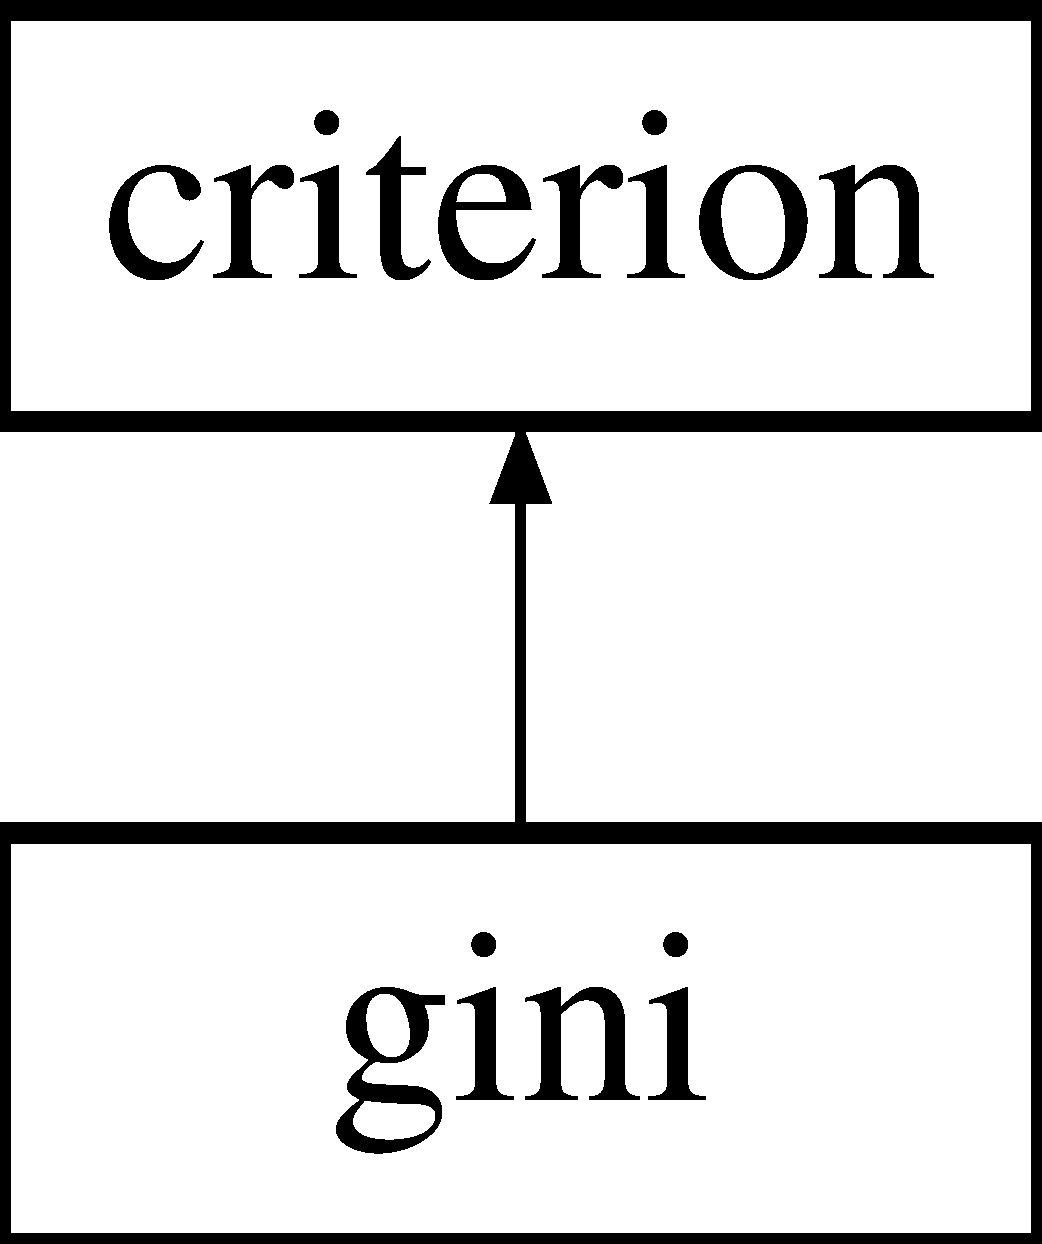
\includegraphics[height=2.000000cm]{classgini}
\end{center}
\end{figure}
\subsection*{Public Member Functions}
\begin{DoxyCompactItemize}
\item 
\hyperlink{classgini_a6b55cd25f78692dd2c7f29f28c6217be}{gini} (float $\ast$\&frequency, int n\+\_\+classes)
\begin{DoxyCompactList}\small\item\em Constructor. \end{DoxyCompactList}\item 
\hyperlink{classgini_ab9bb0e64623a6bf233365bcde20585b0}{$\sim$gini} ()
\begin{DoxyCompactList}\small\item\em $\sim$gini Destructor \end{DoxyCompactList}\item 
float \hyperlink{classgini_a5f232df1155fe182eee9b26cde0e8339}{measure} (float $\ast$\&frequency, int n\+\_\+classes)
\begin{DoxyCompactList}\small\item\em Heuristic measure value. \end{DoxyCompactList}\end{DoxyCompactItemize}
\subsection*{Additional Inherited Members}


\subsection{Detailed Description}
Gini index. 

\subsection{Constructor \& Destructor Documentation}
\hypertarget{classgini_a6b55cd25f78692dd2c7f29f28c6217be}{\index{gini@{gini}!gini@{gini}}
\index{gini@{gini}!gini@{gini}}
\subsubsection[{gini}]{\setlength{\rightskip}{0pt plus 5cm}gini\+::gini (
\begin{DoxyParamCaption}
\item[{float $\ast$\&}]{frequency, }
\item[{int}]{n\+\_\+classes}
\end{DoxyParamCaption}
)}}\label{classgini_a6b55cd25f78692dd2c7f29f28c6217be}


Constructor. 


\begin{DoxyParams}{Parameters}
{\em frequency} & frequency for each class in parent node (sum of each example's weight) \\
\hline
{\em n\+\_\+classes} & number of different classes \\
\hline
\end{DoxyParams}
\hypertarget{classgini_ab9bb0e64623a6bf233365bcde20585b0}{\index{gini@{gini}!````~gini@{$\sim$gini}}
\index{````~gini@{$\sim$gini}!gini@{gini}}
\subsubsection[{$\sim$gini}]{\setlength{\rightskip}{0pt plus 5cm}gini\+::$\sim$gini (
\begin{DoxyParamCaption}
{}
\end{DoxyParamCaption}
)}}\label{classgini_ab9bb0e64623a6bf233365bcde20585b0}


$\sim$gini Destructor 



\subsection{Member Function Documentation}
\hypertarget{classgini_a5f232df1155fe182eee9b26cde0e8339}{\index{gini@{gini}!measure@{measure}}
\index{measure@{measure}!gini@{gini}}
\subsubsection[{measure}]{\setlength{\rightskip}{0pt plus 5cm}float gini\+::measure (
\begin{DoxyParamCaption}
\item[{float $\ast$\&}]{frequency, }
\item[{int}]{n\+\_\+classes}
\end{DoxyParamCaption}
)\hspace{0.3cm}{\ttfamily [virtual]}}}\label{classgini_a5f232df1155fe182eee9b26cde0e8339}


Heuristic measure value. 


\begin{DoxyParams}{Parameters}
{\em frequency} & frequency for each class in the node \\
\hline
{\em n\+\_\+classes} & number of different classes\\
\hline
\end{DoxyParams}
\begin{DoxyReturn}{Returns}
heuristic measure value 
\end{DoxyReturn}


Implements \hyperlink{classcriterion_a1fbda0723578acd5ac612248a54ba71d}{criterion}.



The documentation for this class was generated from the following files\+:\begin{DoxyCompactItemize}
\item 
include/\hyperlink{tree_8h}{tree.\+h}\item 
src/\hyperlink{tree_8cpp}{tree.\+cpp}\end{DoxyCompactItemize}

\hypertarget{classnode}{\section{node Class Reference}
\label{classnode}\index{node@{node}}
}


An abstract class for node in the tree.  




{\ttfamily \#include $<$tree.\+h$>$}

Inheritance diagram for node\+:\begin{figure}[H]
\begin{center}
\leavevmode
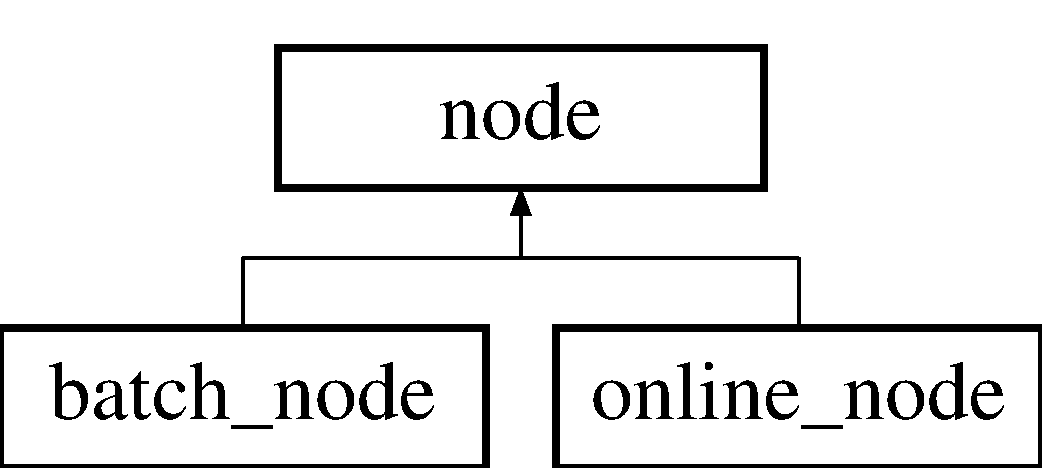
\includegraphics[height=2.000000cm]{classnode}
\end{center}
\end{figure}
\subsection*{Public Member Functions}
\begin{DoxyCompactItemize}
\item 
\hyperlink{classnode_a7e5f4a2e917fe20d91d75faf2e9ba5de}{node} (int \hyperlink{classnode_a8c4864582cb3fe15e84e7908d0965150}{n\+\_\+classes})
\begin{DoxyCompactList}\small\item\em Constructor. \end{DoxyCompactList}\item 
\hyperlink{classnode_a482f83436a89f09d289b26144d817adf}{$\sim$node} ()
\begin{DoxyCompactList}\small\item\em Destructor. \end{DoxyCompactList}\item 
void \hyperlink{classnode_a873438b420d0f6d2659a1b25875ed300}{dump} (const std\+::string \&filename)
\begin{DoxyCompactList}\small\item\em Dump an single node to a binary file. \end{DoxyCompactList}\item 
void \hyperlink{classnode_acab00fde3bcc5d44044c39a37313b4eb}{dump} (std\+::ofstream \&ofs)
\begin{DoxyCompactList}\small\item\em Dump an single node to the output file stream. \end{DoxyCompactList}\item 
void \hyperlink{classnode_a6a92c412ae9336cc7ca5f4575a6384c8}{load} (const std\+::string \&filename)
\begin{DoxyCompactList}\small\item\em load Load an single node from a binary file \end{DoxyCompactList}\item 
void \hyperlink{classnode_a6a25c31eb4c3e8c05d5b70b6bd06adff}{load} (std\+::ifstream \&ifs)
\begin{DoxyCompactList}\small\item\em load Load an single node from the input file stream \end{DoxyCompactList}\item 
void \hyperlink{classnode_a95d492b993f2bd1b59c2489e7eb20a13}{print\+\_\+info} ()
\end{DoxyCompactItemize}
\subsection*{Public Attributes}
\begin{DoxyCompactItemize}
\item 
bool \hyperlink{classnode_a67c3c0be5001ace8494a6292e8079001}{is\+\_\+cate}
\item 
int \hyperlink{classnode_ad65aefa2c967c82cd88e6870085d7f3e}{feature\+\_\+id}
\item 
\hyperlink{dataset_8h_ac2e4791c62a663377be91b0922cede72}{feature\+\_\+t} \hyperlink{classnode_a3774a77cb58d1554f63f34cbcb737a0c}{threshold}
\item 
float \hyperlink{classnode_a7154054210920a77711f8ddb0cf45941}{gain}
\item 
int \hyperlink{classnode_a8c4864582cb3fe15e84e7908d0965150}{n\+\_\+classes}
\item 
float $\ast$ \hyperlink{classnode_ae4125b554711d8ad9d6726ffd69e0b77}{cur\+\_\+frequency}
\item 
int \hyperlink{classnode_abbd7d4174869fead5f901b042a2f9712}{leaf\+\_\+idx}
\item 
\hyperlink{classnode}{node} $\ast$ \hyperlink{classnode_a7cbff55ff448f557223f79299056e9b1}{left}
\item 
\hyperlink{classnode}{node} $\ast$ \hyperlink{classnode_abdc86d4c8604c481752953af3235fc47}{right}
\end{DoxyCompactItemize}


\subsection{Detailed Description}
An abstract class for node in the tree. 

\subsection{Constructor \& Destructor Documentation}
\hypertarget{classnode_a7e5f4a2e917fe20d91d75faf2e9ba5de}{\index{node@{node}!node@{node}}
\index{node@{node}!node@{node}}
\subsubsection[{node}]{\setlength{\rightskip}{0pt plus 5cm}node\+::node (
\begin{DoxyParamCaption}
\item[{int}]{n\+\_\+classes}
\end{DoxyParamCaption}
)}}\label{classnode_a7e5f4a2e917fe20d91d75faf2e9ba5de}


Constructor. 

point to right node 
\begin{DoxyParams}{Parameters}
{\em n\+\_\+classes} & number of different class \\
\hline
\end{DoxyParams}
\hypertarget{classnode_a482f83436a89f09d289b26144d817adf}{\index{node@{node}!````~node@{$\sim$node}}
\index{````~node@{$\sim$node}!node@{node}}
\subsubsection[{$\sim$node}]{\setlength{\rightskip}{0pt plus 5cm}node\+::$\sim$node (
\begin{DoxyParamCaption}
{}
\end{DoxyParamCaption}
)}}\label{classnode_a482f83436a89f09d289b26144d817adf}


Destructor. 



\subsection{Member Function Documentation}
\hypertarget{classnode_a873438b420d0f6d2659a1b25875ed300}{\index{node@{node}!dump@{dump}}
\index{dump@{dump}!node@{node}}
\subsubsection[{dump}]{\setlength{\rightskip}{0pt plus 5cm}void node\+::dump (
\begin{DoxyParamCaption}
\item[{const std\+::string \&}]{filename}
\end{DoxyParamCaption}
)}}\label{classnode_a873438b420d0f6d2659a1b25875ed300}


Dump an single node to a binary file. 


\begin{DoxyParams}{Parameters}
{\em filename} & path to dump \\
\hline
\end{DoxyParams}
\hypertarget{classnode_acab00fde3bcc5d44044c39a37313b4eb}{\index{node@{node}!dump@{dump}}
\index{dump@{dump}!node@{node}}
\subsubsection[{dump}]{\setlength{\rightskip}{0pt plus 5cm}void node\+::dump (
\begin{DoxyParamCaption}
\item[{std\+::ofstream \&}]{ofs}
\end{DoxyParamCaption}
)}}\label{classnode_acab00fde3bcc5d44044c39a37313b4eb}


Dump an single node to the output file stream. 


\begin{DoxyParams}{Parameters}
{\em ofs} & output file stream (should be open first, did not close in this function) \\
\hline
\end{DoxyParams}
\hypertarget{classnode_a6a92c412ae9336cc7ca5f4575a6384c8}{\index{node@{node}!load@{load}}
\index{load@{load}!node@{node}}
\subsubsection[{load}]{\setlength{\rightskip}{0pt plus 5cm}void node\+::load (
\begin{DoxyParamCaption}
\item[{const std\+::string \&}]{filename}
\end{DoxyParamCaption}
)}}\label{classnode_a6a92c412ae9336cc7ca5f4575a6384c8}


load Load an single node from a binary file 


\begin{DoxyParams}{Parameters}
{\em filename} & path to load\\
\hline
\end{DoxyParams}
\begin{DoxyReturn}{Returns}
a node 
\end{DoxyReturn}
\hypertarget{classnode_a6a25c31eb4c3e8c05d5b70b6bd06adff}{\index{node@{node}!load@{load}}
\index{load@{load}!node@{node}}
\subsubsection[{load}]{\setlength{\rightskip}{0pt plus 5cm}void node\+::load (
\begin{DoxyParamCaption}
\item[{std\+::ifstream \&}]{ifs}
\end{DoxyParamCaption}
)}}\label{classnode_a6a25c31eb4c3e8c05d5b70b6bd06adff}


load Load an single node from the input file stream 


\begin{DoxyParams}{Parameters}
{\em ifs} & input file stream (should be open first, did not close in this function)\\
\hline
\end{DoxyParams}
\begin{DoxyReturn}{Returns}
a node 
\end{DoxyReturn}
\hypertarget{classnode_a95d492b993f2bd1b59c2489e7eb20a13}{\index{node@{node}!print\+\_\+info@{print\+\_\+info}}
\index{print\+\_\+info@{print\+\_\+info}!node@{node}}
\subsubsection[{print\+\_\+info}]{\setlength{\rightskip}{0pt plus 5cm}void node\+::print\+\_\+info (
\begin{DoxyParamCaption}
{}
\end{DoxyParamCaption}
)}}\label{classnode_a95d492b993f2bd1b59c2489e7eb20a13}


\subsection{Member Data Documentation}
\hypertarget{classnode_ae4125b554711d8ad9d6726ffd69e0b77}{\index{node@{node}!cur\+\_\+frequency@{cur\+\_\+frequency}}
\index{cur\+\_\+frequency@{cur\+\_\+frequency}!node@{node}}
\subsubsection[{cur\+\_\+frequency}]{\setlength{\rightskip}{0pt plus 5cm}float$\ast$ node\+::cur\+\_\+frequency}}\label{classnode_ae4125b554711d8ad9d6726ffd69e0b77}
number of different class in the node \hypertarget{classnode_ad65aefa2c967c82cd88e6870085d7f3e}{\index{node@{node}!feature\+\_\+id@{feature\+\_\+id}}
\index{feature\+\_\+id@{feature\+\_\+id}!node@{node}}
\subsubsection[{feature\+\_\+id}]{\setlength{\rightskip}{0pt plus 5cm}int node\+::feature\+\_\+id}}\label{classnode_ad65aefa2c967c82cd88e6870085d7f3e}
is the split feature categorical \hypertarget{classnode_a7154054210920a77711f8ddb0cf45941}{\index{node@{node}!gain@{gain}}
\index{gain@{gain}!node@{node}}
\subsubsection[{gain}]{\setlength{\rightskip}{0pt plus 5cm}float node\+::gain}}\label{classnode_a7154054210920a77711f8ddb0cf45941}
for categorical attribute is the chosen feature value for left child node, for continous attribute is the threshold to determine left or right \hypertarget{classnode_a67c3c0be5001ace8494a6292e8079001}{\index{node@{node}!is\+\_\+cate@{is\+\_\+cate}}
\index{is\+\_\+cate@{is\+\_\+cate}!node@{node}}
\subsubsection[{is\+\_\+cate}]{\setlength{\rightskip}{0pt plus 5cm}bool node\+::is\+\_\+cate}}\label{classnode_a67c3c0be5001ace8494a6292e8079001}
\hypertarget{classnode_abbd7d4174869fead5f901b042a2f9712}{\index{node@{node}!leaf\+\_\+idx@{leaf\+\_\+idx}}
\index{leaf\+\_\+idx@{leaf\+\_\+idx}!node@{node}}
\subsubsection[{leaf\+\_\+idx}]{\setlength{\rightskip}{0pt plus 5cm}int node\+::leaf\+\_\+idx}}\label{classnode_abbd7d4174869fead5f901b042a2f9712}
size should be {\ttfamily n\+\_\+classes}, means the weighted frequency for each class \hypertarget{classnode_a7cbff55ff448f557223f79299056e9b1}{\index{node@{node}!left@{left}}
\index{left@{left}!node@{node}}
\subsubsection[{left}]{\setlength{\rightskip}{0pt plus 5cm}{\bf node}$\ast$ node\+::left}}\label{classnode_a7cbff55ff448f557223f79299056e9b1}
-\/1 if this node is not leaf otherwise non-\/negtive integer \hypertarget{classnode_a8c4864582cb3fe15e84e7908d0965150}{\index{node@{node}!n\+\_\+classes@{n\+\_\+classes}}
\index{n\+\_\+classes@{n\+\_\+classes}!node@{node}}
\subsubsection[{n\+\_\+classes}]{\setlength{\rightskip}{0pt plus 5cm}int node\+::n\+\_\+classes}}\label{classnode_a8c4864582cb3fe15e84e7908d0965150}
heuristic measure(e.\+g. gini index or information gain) \hypertarget{classnode_abdc86d4c8604c481752953af3235fc47}{\index{node@{node}!right@{right}}
\index{right@{right}!node@{node}}
\subsubsection[{right}]{\setlength{\rightskip}{0pt plus 5cm}{\bf node}$\ast$ node\+::right}}\label{classnode_abdc86d4c8604c481752953af3235fc47}
point to left node \hypertarget{classnode_a3774a77cb58d1554f63f34cbcb737a0c}{\index{node@{node}!threshold@{threshold}}
\index{threshold@{threshold}!node@{node}}
\subsubsection[{threshold}]{\setlength{\rightskip}{0pt plus 5cm}{\bf feature\+\_\+t} node\+::threshold}}\label{classnode_a3774a77cb58d1554f63f34cbcb737a0c}
split feature id 

The documentation for this class was generated from the following files\+:\begin{DoxyCompactItemize}
\item 
\hyperlink{tree_8h}{tree.\+h}\item 
\hyperlink{tree_8cpp}{tree.\+cpp}\end{DoxyCompactItemize}

\hypertarget{classonline__node}{\section{online\+\_\+node Class Reference}
\label{classonline__node}\index{online\+\_\+node@{online\+\_\+node}}
}


Specify for online tree algorithm.  




{\ttfamily \#include $<$tree.\+h$>$}

Inheritance diagram for online\+\_\+node\+:\begin{figure}[H]
\begin{center}
\leavevmode
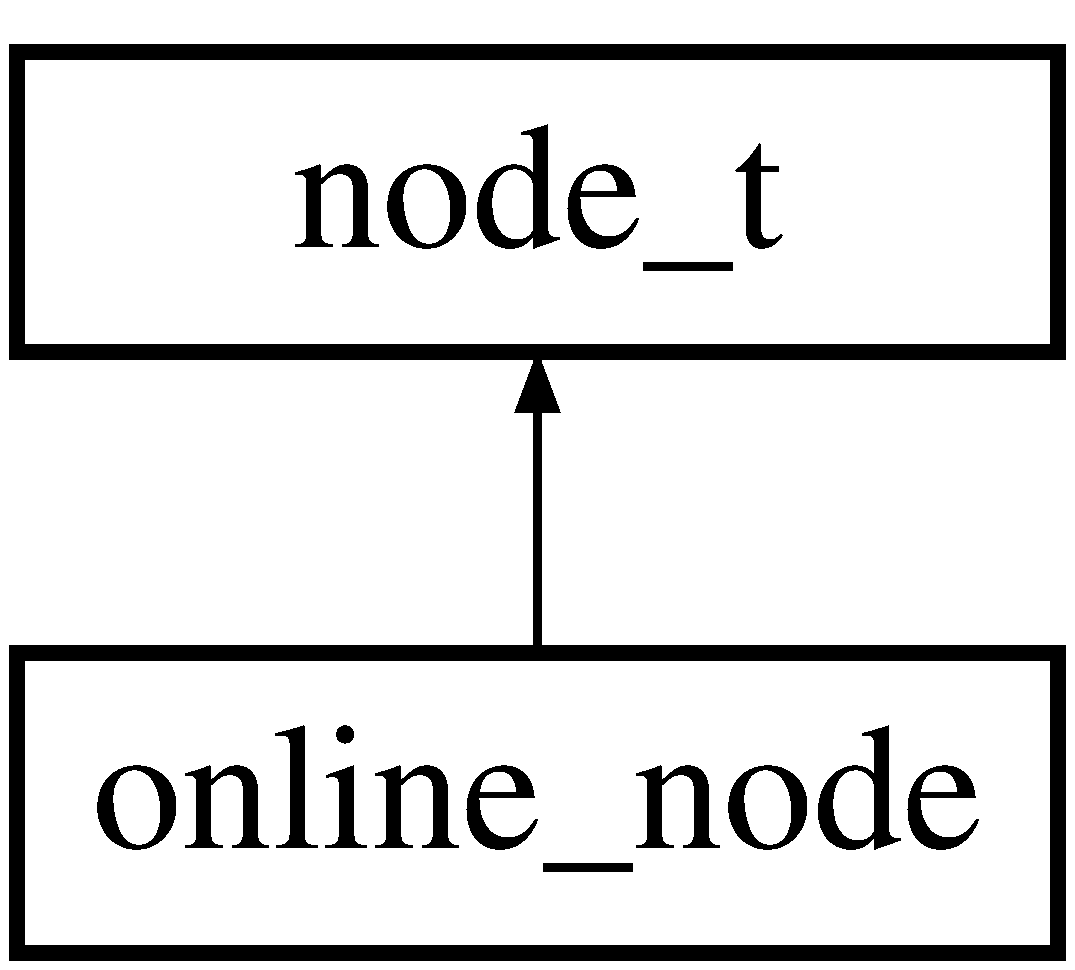
\includegraphics[height=2.000000cm]{classonline__node}
\end{center}
\end{figure}
\subsection*{Additional Inherited Members}


\subsection{Detailed Description}
Specify for online tree algorithm. 

The documentation for this class was generated from the following file\+:\begin{DoxyCompactItemize}
\item 
\hyperlink{tree_8h}{tree.\+h}\end{DoxyCompactItemize}

\hypertarget{classonline__tree}{\section{online\+\_\+tree Class Reference}
\label{classonline__tree}\index{online\+\_\+tree@{online\+\_\+tree}}
}


Online Decision Tree Classifier.  




{\ttfamily \#include $<$tree.\+h$>$}

Inheritance diagram for online\+\_\+tree\+:\begin{figure}[H]
\begin{center}
\leavevmode
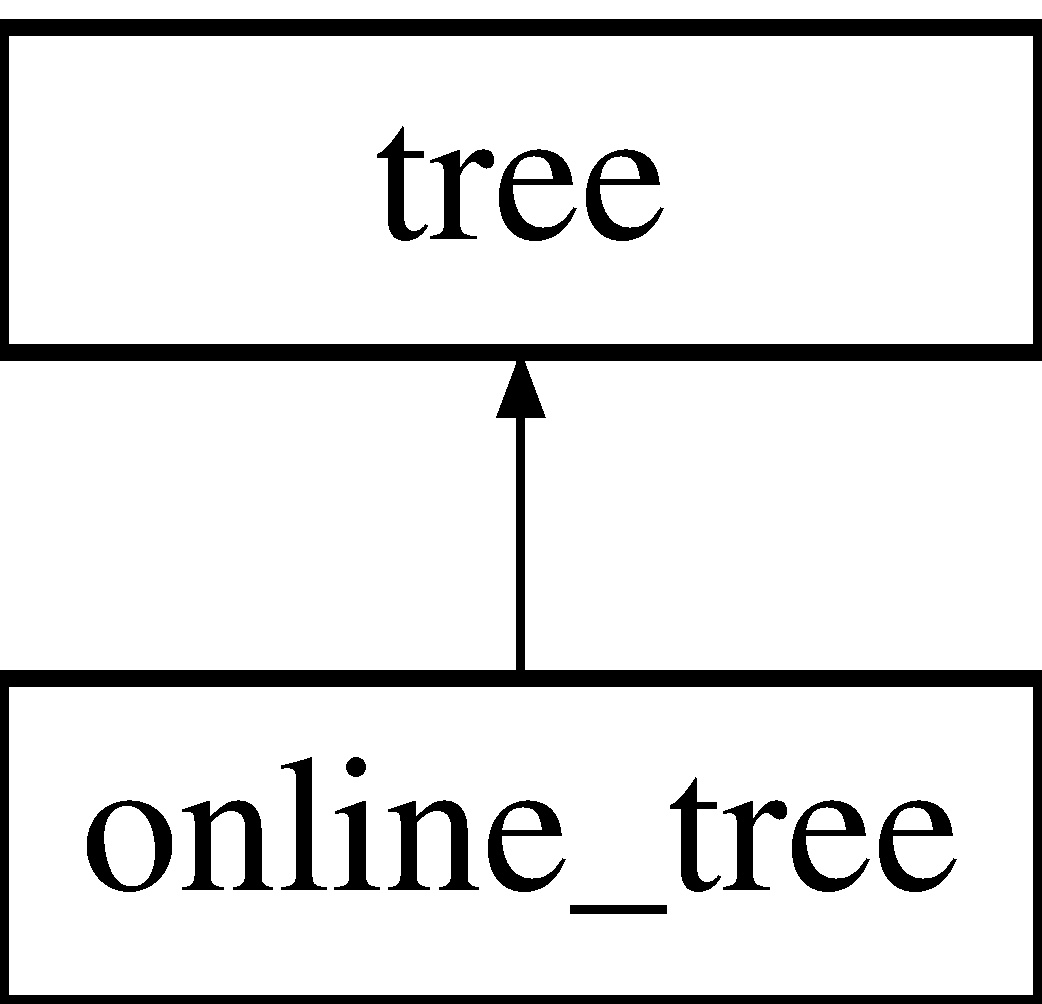
\includegraphics[height=2.000000cm]{classonline__tree}
\end{center}
\end{figure}
\subsection*{Additional Inherited Members}


\subsection{Detailed Description}
Online Decision Tree Classifier. 

The documentation for this class was generated from the following file\+:\begin{DoxyCompactItemize}
\item 
\hyperlink{tree_8h}{tree.\+h}\end{DoxyCompactItemize}

\hypertarget{classrandom__splitter}{\section{random\+\_\+splitter Class Reference}
\label{classrandom__splitter}\index{random\+\_\+splitter@{random\+\_\+splitter}}
}


Test some random threshold to choose a best split among these.  




{\ttfamily \#include $<$tree.\+h$>$}

Inheritance diagram for random\+\_\+splitter\+:\begin{figure}[H]
\begin{center}
\leavevmode
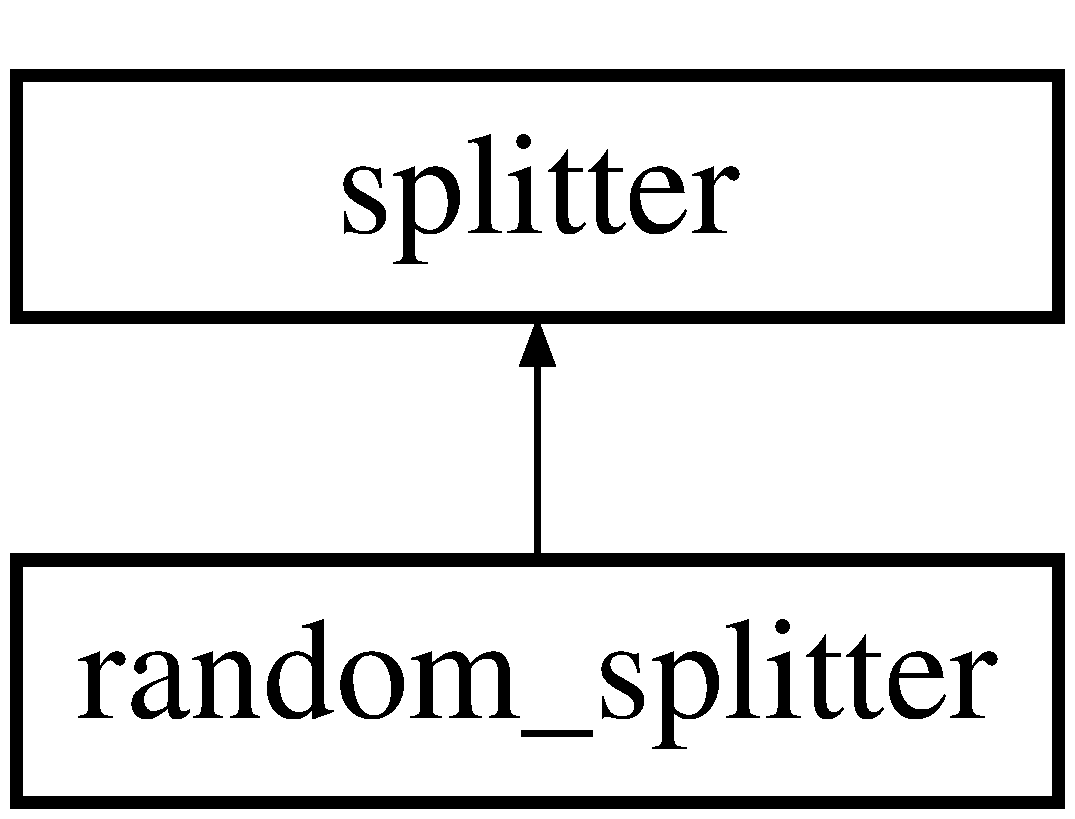
\includegraphics[height=2.000000cm]{classrandom__splitter}
\end{center}
\end{figure}
\subsection*{Additional Inherited Members}


\subsection{Detailed Description}
Test some random threshold to choose a best split among these. 

The documentation for this class was generated from the following file\+:\begin{DoxyCompactItemize}
\item 
include/\hyperlink{tree_8h}{tree.\+h}\end{DoxyCompactItemize}

\hypertarget{class_random_forest_classifier}{\section{Random\+Forest\+Classifier Class Reference}
\label{class_random_forest_classifier}\index{Random\+Forest\+Classifier@{Random\+Forest\+Classifier}}
}


{\ttfamily \#include $<$forest.\+h$>$}

Inheritance diagram for Random\+Forest\+Classifier\+:\begin{figure}[H]
\begin{center}
\leavevmode
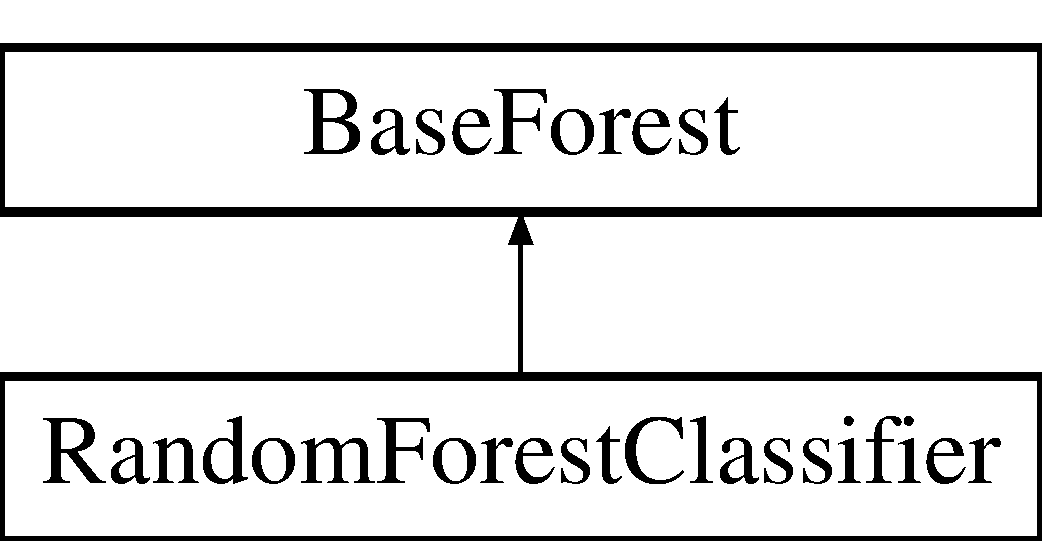
\includegraphics[height=2.000000cm]{class_random_forest_classifier}
\end{center}
\end{figure}
\subsection*{Public Member Functions}
\begin{DoxyCompactItemize}
\item 
\hyperlink{class_random_forest_classifier_af10e2093a8e33384ded4aa30b8cbe4e4}{Random\+Forest\+Classifier} ()
\item 
\hyperlink{class_random_forest_classifier_a18ef391e71da976b924013c5c26cbe44}{Random\+Forest\+Classifier} (int \hyperlink{class_base_forest_a2549a0057ec5419fe1de52ef198125ce}{n\+\_\+trees}, int \hyperlink{class_base_forest_a94fe86e1b426d149a11d100921cea3a4}{n\+\_\+threads}=\hyperlink{class_base_forest_a36733c1fadd0daadba8e694ee30fd1b6}{D\+E\+F\+A\+U\+L\+T\+\_\+\+N\+\_\+\+T\+H\+R\+E\+A\+D\+S}, std\+::string \hyperlink{class_base_forest_a5c651ace1f9d5177cdff38a0ae4048f7}{max\+\_\+feature\+\_\+criterion}=\char`\"{}sqrt\char`\"{}, int \hyperlink{class_base_forest_a85cf2e2e202c6e82bf684057181138f6}{max\+\_\+depth}=\hyperlink{class_base_forest_ac6df44eee4d7ee5913ad57d1d6c79692}{D\+E\+F\+A\+U\+L\+T\+\_\+\+M\+A\+X\+\_\+\+D\+E\+P\+T\+H}, int \hyperlink{class_base_forest_a15e0407f3c0fbc4c25e0796c781ff059}{min\+\_\+leaf\+\_\+samples}=\hyperlink{class_base_forest_a3d000d7f9e2410c73b41b70d8e2e58f8}{D\+E\+F\+A\+U\+L\+T\+\_\+\+M\+I\+N\+\_\+\+L\+E\+A\+F\+\_\+\+S\+A\+M\+P\+L\+E\+S})
\item 
void \hyperlink{class_random_forest_classifier_a07680b59615bb765843e3eec4139365e}{train} (std\+::string filename, int feature\+\_\+size, bool is\+\_\+text, int $\ast$discrete\+\_\+idx=N\+U\+L\+L, int discrete\+\_\+size=0, double $\ast$class\+\_\+weight=N\+U\+L\+L)
\item 
void \hyperlink{class_random_forest_classifier_a8a397b32e0f6ba43ecfb669ed9bc07e5}{train} (std\+::string feature\+\_\+filename, std\+::string label\+\_\+filename, int feature\+\_\+size, int \hyperlink{class_base_forest_a07e8b0ed27405f469198f2c4875786c9}{max\+\_\+feature}, int $\ast$discrete\+\_\+idx=N\+U\+L\+L, int discrete\+\_\+size=0, double $\ast$class\+\_\+weight=N\+U\+L\+L)
\end{DoxyCompactItemize}
\subsection*{Private Member Functions}
\begin{DoxyCompactItemize}
\item 
void \hyperlink{class_random_forest_classifier_a0a8a6b33668d878c0fc6772fc63c5ebf}{init} (int \hyperlink{class_base_forest_a2549a0057ec5419fe1de52ef198125ce}{n\+\_\+trees}, int \hyperlink{class_base_forest_a94fe86e1b426d149a11d100921cea3a4}{n\+\_\+threads}, int \hyperlink{class_base_forest_a85cf2e2e202c6e82bf684057181138f6}{max\+\_\+depth}, int \hyperlink{class_base_forest_a15e0407f3c0fbc4c25e0796c781ff059}{min\+\_\+leaf\+\_\+samples})
\item 
int \hyperlink{class_random_forest_classifier_a9fa7824a40995e37838c34e296538487}{compute\+\_\+max\+\_\+feature} (int feature\+\_\+size)
\item 
void \hyperlink{class_random_forest_classifier_a4298934ca4d0a44814c6d10f83aee2bf}{parallel\+\_\+build\+\_\+forest} (int tree\+\_\+start, int tree\+\_\+end, double $\ast$class\+\_\+weight)
\item 
void \hyperlink{class_random_forest_classifier_ae46a41b04945bd42658945769c5f4e24}{build\+\_\+forest} (double $\ast$class\+\_\+weight)
\end{DoxyCompactItemize}
\subsection*{Additional Inherited Members}


\subsection{Constructor \& Destructor Documentation}
\hypertarget{class_random_forest_classifier_af10e2093a8e33384ded4aa30b8cbe4e4}{\index{Random\+Forest\+Classifier@{Random\+Forest\+Classifier}!Random\+Forest\+Classifier@{Random\+Forest\+Classifier}}
\index{Random\+Forest\+Classifier@{Random\+Forest\+Classifier}!Random\+Forest\+Classifier@{Random\+Forest\+Classifier}}
\subsubsection[{Random\+Forest\+Classifier}]{\setlength{\rightskip}{0pt plus 5cm}Random\+Forest\+Classifier\+::\+Random\+Forest\+Classifier (
\begin{DoxyParamCaption}
{}
\end{DoxyParamCaption}
)}}\label{class_random_forest_classifier_af10e2093a8e33384ded4aa30b8cbe4e4}
\hypertarget{class_random_forest_classifier_a18ef391e71da976b924013c5c26cbe44}{\index{Random\+Forest\+Classifier@{Random\+Forest\+Classifier}!Random\+Forest\+Classifier@{Random\+Forest\+Classifier}}
\index{Random\+Forest\+Classifier@{Random\+Forest\+Classifier}!Random\+Forest\+Classifier@{Random\+Forest\+Classifier}}
\subsubsection[{Random\+Forest\+Classifier}]{\setlength{\rightskip}{0pt plus 5cm}Random\+Forest\+Classifier\+::\+Random\+Forest\+Classifier (
\begin{DoxyParamCaption}
\item[{int}]{n\+\_\+trees, }
\item[{int}]{n\+\_\+threads = {\ttfamily {\bf D\+E\+F\+A\+U\+L\+T\+\_\+\+N\+\_\+\+T\+H\+R\+E\+A\+D\+S}}, }
\item[{std\+::string}]{max\+\_\+feature\+\_\+criterion = {\ttfamily \char`\"{}sqrt\char`\"{}}, }
\item[{int}]{max\+\_\+depth = {\ttfamily {\bf D\+E\+F\+A\+U\+L\+T\+\_\+\+M\+A\+X\+\_\+\+D\+E\+P\+T\+H}}, }
\item[{int}]{min\+\_\+leaf\+\_\+samples = {\ttfamily {\bf D\+E\+F\+A\+U\+L\+T\+\_\+\+M\+I\+N\+\_\+\+L\+E\+A\+F\+\_\+\+S\+A\+M\+P\+L\+E\+S}}}
\end{DoxyParamCaption}
)}}\label{class_random_forest_classifier_a18ef391e71da976b924013c5c26cbe44}


\subsection{Member Function Documentation}
\hypertarget{class_random_forest_classifier_ae46a41b04945bd42658945769c5f4e24}{\index{Random\+Forest\+Classifier@{Random\+Forest\+Classifier}!build\+\_\+forest@{build\+\_\+forest}}
\index{build\+\_\+forest@{build\+\_\+forest}!Random\+Forest\+Classifier@{Random\+Forest\+Classifier}}
\subsubsection[{build\+\_\+forest}]{\setlength{\rightskip}{0pt plus 5cm}void Random\+Forest\+Classifier\+::build\+\_\+forest (
\begin{DoxyParamCaption}
\item[{double $\ast$}]{class\+\_\+weight}
\end{DoxyParamCaption}
)\hspace{0.3cm}{\ttfamily [private]}}}\label{class_random_forest_classifier_ae46a41b04945bd42658945769c5f4e24}
\hypertarget{class_random_forest_classifier_a9fa7824a40995e37838c34e296538487}{\index{Random\+Forest\+Classifier@{Random\+Forest\+Classifier}!compute\+\_\+max\+\_\+feature@{compute\+\_\+max\+\_\+feature}}
\index{compute\+\_\+max\+\_\+feature@{compute\+\_\+max\+\_\+feature}!Random\+Forest\+Classifier@{Random\+Forest\+Classifier}}
\subsubsection[{compute\+\_\+max\+\_\+feature}]{\setlength{\rightskip}{0pt plus 5cm}int Random\+Forest\+Classifier\+::compute\+\_\+max\+\_\+feature (
\begin{DoxyParamCaption}
\item[{int}]{feature\+\_\+size}
\end{DoxyParamCaption}
)\hspace{0.3cm}{\ttfamily [private]}}}\label{class_random_forest_classifier_a9fa7824a40995e37838c34e296538487}
\hypertarget{class_random_forest_classifier_a0a8a6b33668d878c0fc6772fc63c5ebf}{\index{Random\+Forest\+Classifier@{Random\+Forest\+Classifier}!init@{init}}
\index{init@{init}!Random\+Forest\+Classifier@{Random\+Forest\+Classifier}}
\subsubsection[{init}]{\setlength{\rightskip}{0pt plus 5cm}void Random\+Forest\+Classifier\+::init (
\begin{DoxyParamCaption}
\item[{int}]{n\+\_\+trees, }
\item[{int}]{n\+\_\+threads, }
\item[{int}]{max\+\_\+depth, }
\item[{int}]{min\+\_\+leaf\+\_\+samples}
\end{DoxyParamCaption}
)\hspace{0.3cm}{\ttfamily [private]}}}\label{class_random_forest_classifier_a0a8a6b33668d878c0fc6772fc63c5ebf}
\hypertarget{class_random_forest_classifier_a4298934ca4d0a44814c6d10f83aee2bf}{\index{Random\+Forest\+Classifier@{Random\+Forest\+Classifier}!parallel\+\_\+build\+\_\+forest@{parallel\+\_\+build\+\_\+forest}}
\index{parallel\+\_\+build\+\_\+forest@{parallel\+\_\+build\+\_\+forest}!Random\+Forest\+Classifier@{Random\+Forest\+Classifier}}
\subsubsection[{parallel\+\_\+build\+\_\+forest}]{\setlength{\rightskip}{0pt plus 5cm}void Random\+Forest\+Classifier\+::parallel\+\_\+build\+\_\+forest (
\begin{DoxyParamCaption}
\item[{int}]{tree\+\_\+start, }
\item[{int}]{tree\+\_\+end, }
\item[{double $\ast$}]{class\+\_\+weight}
\end{DoxyParamCaption}
)\hspace{0.3cm}{\ttfamily [private]}}}\label{class_random_forest_classifier_a4298934ca4d0a44814c6d10f83aee2bf}
\hypertarget{class_random_forest_classifier_a07680b59615bb765843e3eec4139365e}{\index{Random\+Forest\+Classifier@{Random\+Forest\+Classifier}!train@{train}}
\index{train@{train}!Random\+Forest\+Classifier@{Random\+Forest\+Classifier}}
\subsubsection[{train}]{\setlength{\rightskip}{0pt plus 5cm}void Random\+Forest\+Classifier\+::train (
\begin{DoxyParamCaption}
\item[{std\+::string}]{filename, }
\item[{int}]{feature\+\_\+size, }
\item[{bool}]{is\+\_\+text, }
\item[{int $\ast$}]{discrete\+\_\+idx = {\ttfamily NULL}, }
\item[{int}]{discrete\+\_\+size = {\ttfamily 0}, }
\item[{double $\ast$}]{class\+\_\+weight = {\ttfamily NULL}}
\end{DoxyParamCaption}
)}}\label{class_random_forest_classifier_a07680b59615bb765843e3eec4139365e}
\hypertarget{class_random_forest_classifier_a8a397b32e0f6ba43ecfb669ed9bc07e5}{\index{Random\+Forest\+Classifier@{Random\+Forest\+Classifier}!train@{train}}
\index{train@{train}!Random\+Forest\+Classifier@{Random\+Forest\+Classifier}}
\subsubsection[{train}]{\setlength{\rightskip}{0pt plus 5cm}void Random\+Forest\+Classifier\+::train (
\begin{DoxyParamCaption}
\item[{std\+::string}]{feature\+\_\+filename, }
\item[{std\+::string}]{label\+\_\+filename, }
\item[{int}]{feature\+\_\+size, }
\item[{int}]{max\+\_\+feature, }
\item[{int $\ast$}]{discrete\+\_\+idx = {\ttfamily NULL}, }
\item[{int}]{discrete\+\_\+size = {\ttfamily 0}, }
\item[{double $\ast$}]{class\+\_\+weight = {\ttfamily NULL}}
\end{DoxyParamCaption}
)}}\label{class_random_forest_classifier_a8a397b32e0f6ba43ecfb669ed9bc07e5}


The documentation for this class was generated from the following files\+:\begin{DoxyCompactItemize}
\item 
\hyperlink{forest_8h}{forest.\+h}\item 
\hyperlink{forest_8cpp}{forest.\+cpp}\end{DoxyCompactItemize}

\hypertarget{classsplitter}{\section{splitter Class Reference}
\label{classsplitter}\index{splitter@{splitter}}
}


Abstract class which is used to split the node.  




{\ttfamily \#include $<$tree.\+h$>$}

Inheritance diagram for splitter\+:\begin{figure}[H]
\begin{center}
\leavevmode
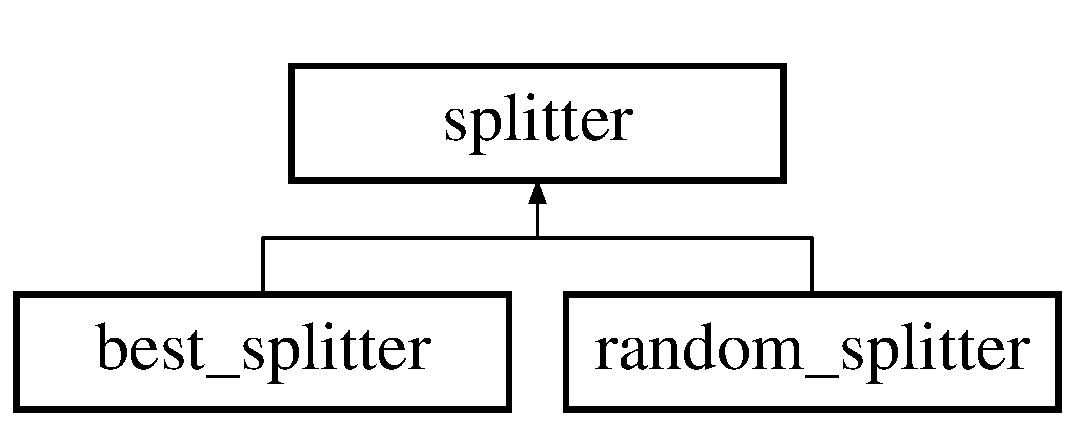
\includegraphics[height=2.000000cm]{classsplitter}
\end{center}
\end{figure}
\subsection*{Public Member Functions}
\begin{DoxyCompactItemize}
\item 
\hyperlink{classsplitter_aecf4cc04f2ae39a4a8e13d4049d442cf}{splitter} (int \hyperlink{classsplitter_abfc53538ed65c0afd50aedbf46dff458}{n\+\_\+classes})
\begin{DoxyCompactList}\small\item\em Constructor. \end{DoxyCompactList}\item 
virtual \hyperlink{classsplitter_a221bcb6b6705bb240ef6eea0c95f841a}{$\sim$splitter} ()
\begin{DoxyCompactList}\small\item\em Destructor. \end{DoxyCompactList}\item 
virtual void \hyperlink{classsplitter_af592533ea2d8d16337fa6c8a9a0a6b36}{split} (\hyperlink{classtree}{tree} $\ast$t, \hyperlink{classnode}{node} $\ast$\&root, \hyperlink{classdataset}{dataset} $\ast$\&d, \hyperlink{classcriterion}{criterion} $\ast$\&cr)=0
\begin{DoxyCompactList}\small\item\em Choose a split. \end{DoxyCompactList}\end{DoxyCompactItemize}
\subsection*{Public Attributes}
\begin{DoxyCompactItemize}
\item 
int \hyperlink{classsplitter_ad093754efc111ae9dcb00e844b91e979}{fea\+\_\+id}
\item 
float \hyperlink{classsplitter_af40121f8411ad94f3f1968b1d50905ed}{threshold}
\item 
float \hyperlink{classsplitter_a4c49114e4256e0dca9ead72f3ecb5a74}{gain}
\item 
int \hyperlink{classsplitter_abfc53538ed65c0afd50aedbf46dff458}{n\+\_\+classes}
\item 
float $\ast$ \hyperlink{classsplitter_a0a1c53a640e3305eeb32a9586fea657b}{left\+\_\+frequency}
\item 
float $\ast$ \hyperlink{classsplitter_a8e1727de05ad39513dab201d6657aeed}{right\+\_\+frequency}
\end{DoxyCompactItemize}
\subsection*{Protected Member Functions}
\begin{DoxyCompactItemize}
\item 
virtual void \hyperlink{classsplitter_ab2ea956cc1a10ebb39422fa5ac450af2}{update} (int \hyperlink{classsplitter_ad093754efc111ae9dcb00e844b91e979}{fea\+\_\+id}, float \hyperlink{classsplitter_af40121f8411ad94f3f1968b1d50905ed}{threshold}, float $\ast$\&left, \hyperlink{classnode}{node} $\ast$\&nd, \hyperlink{classcriterion}{criterion} $\ast$\&cr)=0
\begin{DoxyCompactList}\small\item\em Update the split information (e.\+g. split feature id, threshold, gain, etc.) if this candidate split is better. \end{DoxyCompactList}\end{DoxyCompactItemize}


\subsection{Detailed Description}
Abstract class which is used to split the node. 

\subsection{Constructor \& Destructor Documentation}
\hypertarget{classsplitter_aecf4cc04f2ae39a4a8e13d4049d442cf}{\index{splitter@{splitter}!splitter@{splitter}}
\index{splitter@{splitter}!splitter@{splitter}}
\subsubsection[{splitter}]{\setlength{\rightskip}{0pt plus 5cm}splitter\+::splitter (
\begin{DoxyParamCaption}
\item[{int}]{n\+\_\+classes}
\end{DoxyParamCaption}
)}}\label{classsplitter_aecf4cc04f2ae39a4a8e13d4049d442cf}


Constructor. 

right\mbox{[}j\mbox{]} refers to weighted frequency for class j 
\begin{DoxyParams}{Parameters}
{\em n\+\_\+classes} & number of different classes \\
\hline
\end{DoxyParams}
\hypertarget{classsplitter_a221bcb6b6705bb240ef6eea0c95f841a}{\index{splitter@{splitter}!````~splitter@{$\sim$splitter}}
\index{````~splitter@{$\sim$splitter}!splitter@{splitter}}
\subsubsection[{$\sim$splitter}]{\setlength{\rightskip}{0pt plus 5cm}splitter\+::$\sim$splitter (
\begin{DoxyParamCaption}
{}
\end{DoxyParamCaption}
)\hspace{0.3cm}{\ttfamily [virtual]}}}\label{classsplitter_a221bcb6b6705bb240ef6eea0c95f841a}


Destructor. 



\subsection{Member Function Documentation}
\hypertarget{classsplitter_af592533ea2d8d16337fa6c8a9a0a6b36}{\index{splitter@{splitter}!split@{split}}
\index{split@{split}!splitter@{splitter}}
\subsubsection[{split}]{\setlength{\rightskip}{0pt plus 5cm}virtual void splitter\+::split (
\begin{DoxyParamCaption}
\item[{{\bf tree} $\ast$}]{t, }
\item[{{\bf node} $\ast$\&}]{root, }
\item[{{\bf dataset} $\ast$\&}]{d, }
\item[{{\bf criterion} $\ast$\&}]{cr}
\end{DoxyParamCaption}
)\hspace{0.3cm}{\ttfamily [pure virtual]}}}\label{classsplitter_af592533ea2d8d16337fa6c8a9a0a6b36}


Choose a split. 


\begin{DoxyParams}{Parameters}
{\em t} & tree object \\
\hline
{\em root} & one of the node in tree {\ttfamily t} which is to be splited \\
\hline
{\em d} & training dataset \\
\hline
{\em cr} & criterion to determine the better split (e.\+g. information gain, gini index) \\
\hline
\end{DoxyParams}


Implemented in \hyperlink{classbest__splitter_a1ff1e766bfa4fb6d41c23121d6dd3dbb}{best\+\_\+splitter}.

\hypertarget{classsplitter_ab2ea956cc1a10ebb39422fa5ac450af2}{\index{splitter@{splitter}!update@{update}}
\index{update@{update}!splitter@{splitter}}
\subsubsection[{update}]{\setlength{\rightskip}{0pt plus 5cm}virtual void splitter\+::update (
\begin{DoxyParamCaption}
\item[{int}]{fea\+\_\+id, }
\item[{float}]{threshold, }
\item[{float $\ast$\&}]{left, }
\item[{{\bf node} $\ast$\&}]{nd, }
\item[{{\bf criterion} $\ast$\&}]{cr}
\end{DoxyParamCaption}
)\hspace{0.3cm}{\ttfamily [protected]}, {\ttfamily [pure virtual]}}}\label{classsplitter_ab2ea956cc1a10ebb39422fa5ac450af2}


Update the split information (e.\+g. split feature id, threshold, gain, etc.) if this candidate split is better. 


\begin{DoxyParams}{Parameters}
{\em fea\+\_\+id} & feature id to split \\
\hline
{\em threshold} & threshold of the split (less than {\ttfamily threshold} belong to left node) \\
\hline
{\em left} & pre-\/computed left node's frequency for each class after the split \\
\hline
{\em nd} & the node to split \\
\hline
{\em cr} & criterion to determine the better split (e.\+g. information gain, gini index) \\
\hline
\end{DoxyParams}


Implemented in \hyperlink{classbest__splitter_a681ad1823db5207f3a5a6acd5c09b354}{best\+\_\+splitter}.



\subsection{Member Data Documentation}
\hypertarget{classsplitter_ad093754efc111ae9dcb00e844b91e979}{\index{splitter@{splitter}!fea\+\_\+id@{fea\+\_\+id}}
\index{fea\+\_\+id@{fea\+\_\+id}!splitter@{splitter}}
\subsubsection[{fea\+\_\+id}]{\setlength{\rightskip}{0pt plus 5cm}int splitter\+::fea\+\_\+id}}\label{classsplitter_ad093754efc111ae9dcb00e844b91e979}
\hypertarget{classsplitter_a4c49114e4256e0dca9ead72f3ecb5a74}{\index{splitter@{splitter}!gain@{gain}}
\index{gain@{gain}!splitter@{splitter}}
\subsubsection[{gain}]{\setlength{\rightskip}{0pt plus 5cm}float splitter\+::gain}}\label{classsplitter_a4c49114e4256e0dca9ead72f3ecb5a74}
split threshold \hypertarget{classsplitter_a0a1c53a640e3305eeb32a9586fea657b}{\index{splitter@{splitter}!left\+\_\+frequency@{left\+\_\+frequency}}
\index{left\+\_\+frequency@{left\+\_\+frequency}!splitter@{splitter}}
\subsubsection[{left\+\_\+frequency}]{\setlength{\rightskip}{0pt plus 5cm}float$\ast$ splitter\+::left\+\_\+frequency}}\label{classsplitter_a0a1c53a640e3305eeb32a9586fea657b}
different classes when split \hypertarget{classsplitter_abfc53538ed65c0afd50aedbf46dff458}{\index{splitter@{splitter}!n\+\_\+classes@{n\+\_\+classes}}
\index{n\+\_\+classes@{n\+\_\+classes}!splitter@{splitter}}
\subsubsection[{n\+\_\+classes}]{\setlength{\rightskip}{0pt plus 5cm}int splitter\+::n\+\_\+classes}}\label{classsplitter_abfc53538ed65c0afd50aedbf46dff458}
heuristc measure (e.\+g. information gain or gini index) improvement after split \hypertarget{classsplitter_a8e1727de05ad39513dab201d6657aeed}{\index{splitter@{splitter}!right\+\_\+frequency@{right\+\_\+frequency}}
\index{right\+\_\+frequency@{right\+\_\+frequency}!splitter@{splitter}}
\subsubsection[{right\+\_\+frequency}]{\setlength{\rightskip}{0pt plus 5cm}float$\ast$ splitter\+::right\+\_\+frequency}}\label{classsplitter_a8e1727de05ad39513dab201d6657aeed}
left\mbox{[}j\mbox{]} refers to weighted frequency for class j \hypertarget{classsplitter_af40121f8411ad94f3f1968b1d50905ed}{\index{splitter@{splitter}!threshold@{threshold}}
\index{threshold@{threshold}!splitter@{splitter}}
\subsubsection[{threshold}]{\setlength{\rightskip}{0pt plus 5cm}float splitter\+::threshold}}\label{classsplitter_af40121f8411ad94f3f1968b1d50905ed}
split feature id 

The documentation for this class was generated from the following files\+:\begin{DoxyCompactItemize}
\item 
include/\hyperlink{tree_8h}{tree.\+h}\item 
src/\hyperlink{tree_8cpp}{tree.\+cpp}\end{DoxyCompactItemize}

\hypertarget{classtree}{\section{tree Class Reference}
\label{classtree}\index{tree@{tree}}
}


{\ttfamily \#include $<$tree.\+h$>$}

Inheritance diagram for tree\+:\begin{figure}[H]
\begin{center}
\leavevmode
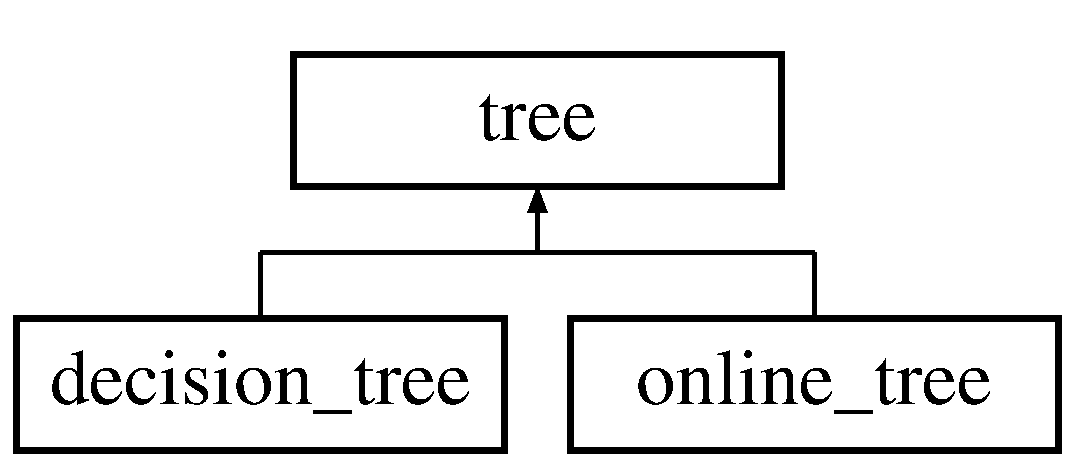
\includegraphics[height=2.000000cm]{classtree}
\end{center}
\end{figure}
\subsection*{Public Member Functions}
\begin{DoxyCompactItemize}
\item 
\hyperlink{classtree_a9f2a566ac2710fafc31232456780e82d}{tree} ()
\item 
\hyperlink{classtree_a05f3faa3c9a8f6fed237e2d0f6172244}{$\sim$tree} ()
\item 
\hyperlink{classtree_a356d6ebfe68b6e4ac466664c4f2d2581}{tree} (const std\+::string \hyperlink{classtree_a5aba3b77a347165517a20d5fab94382d}{feature\+\_\+rule}, int \hyperlink{classtree_a0a9f968fac827d3239be67488c34fb21}{max\+\_\+depth}, int \hyperlink{classtree_ae70cd626c0b50a0b8306a94a9e5e8fd7}{min\+\_\+split})
\item 
void \hyperlink{classtree_a03aebcb3102b4f6503b5bc69288297e8}{init} (const std\+::string \hyperlink{classtree_a5aba3b77a347165517a20d5fab94382d}{feature\+\_\+rule}, int \hyperlink{classtree_a0a9f968fac827d3239be67488c34fb21}{max\+\_\+depth}, int \hyperlink{classtree_ae70cd626c0b50a0b8306a94a9e5e8fd7}{min\+\_\+split})
\item 
float $\ast$ \hyperlink{classtree_ae03f6dd2597846c65c1c037728b06bcd}{compute\+\_\+importance} (bool re\+\_\+compute=false)
\item 
void \hyperlink{classtree_a4ca3902b09e854a76f1fb56bb71599f6}{free\+\_\+tree} (\hyperlink{classnode}{node} $\ast$\&nd)
\item 
void \hyperlink{classtree_a634ee04f1f89801a9f295e11cc5ce149}{dump} (const std\+::string \&filename)
\item 
void \hyperlink{classtree_a680d0cc993c3a3d3ef10c891de69960f}{load} (const std\+::string \&filename)
\item 
void \hyperlink{classtree_abc6048c70de7490eabf2433d46067b7b}{export\+\_\+dotfile} (const std\+::string \&filename)
\item 
int \hyperlink{classtree_a8042d0897915fdfeeca4b4d75515b96c}{get\+\_\+max\+\_\+feature} ()
\end{DoxyCompactItemize}
\subsection*{Public Attributes}
\begin{DoxyCompactItemize}
\item 
int $\ast$ \hyperlink{classtree_afa8e539406e1f8b373b147682e3a8196}{valid}
\end{DoxyCompactItemize}
\subsection*{Protected Attributes}
\begin{DoxyCompactItemize}
\item 
\hyperlink{classnode}{node} $\ast$ \hyperlink{classtree_ad397d4906e47149b98f769b3e81473ee}{root}
\item 
\hyperlink{classnode}{node} $\ast$$\ast$ \hyperlink{classtree_ac697cf1868c26ac26f005e6ee8be9d43}{leaf\+\_\+pt}
\item 
int \hyperlink{classtree_a551919e1402a700821694297623017fc}{leaf\+\_\+size}
\item 
int \hyperlink{classtree_a48430ab4447259c35af5f22e894e1d6c}{n\+\_\+features}
\item 
std\+::string \hyperlink{classtree_a5aba3b77a347165517a20d5fab94382d}{feature\+\_\+rule}
\item 
int \hyperlink{classtree_a6f4304318f8f091f7d783ac1ec7d2775}{max\+\_\+feature}
\item 
int \hyperlink{classtree_a0a9f968fac827d3239be67488c34fb21}{max\+\_\+depth}
\item 
int \hyperlink{classtree_ae70cd626c0b50a0b8306a94a9e5e8fd7}{min\+\_\+split}
\item 
float $\ast$ \hyperlink{classtree_ad335e57b2f4f2326825694311bcc69e7}{fea\+\_\+imp}
\end{DoxyCompactItemize}


\subsection{Constructor \& Destructor Documentation}
\hypertarget{classtree_a9f2a566ac2710fafc31232456780e82d}{\index{tree@{tree}!tree@{tree}}
\index{tree@{tree}!tree@{tree}}
\subsubsection[{tree}]{\setlength{\rightskip}{0pt plus 5cm}tree\+::tree (
\begin{DoxyParamCaption}
{}
\end{DoxyParamCaption}
)}}\label{classtree_a9f2a566ac2710fafc31232456780e82d}
is the example valid to consider when split \hypertarget{classtree_a05f3faa3c9a8f6fed237e2d0f6172244}{\index{tree@{tree}!````~tree@{$\sim$tree}}
\index{````~tree@{$\sim$tree}!tree@{tree}}
\subsubsection[{$\sim$tree}]{\setlength{\rightskip}{0pt plus 5cm}tree\+::$\sim$tree (
\begin{DoxyParamCaption}
{}
\end{DoxyParamCaption}
)}}\label{classtree_a05f3faa3c9a8f6fed237e2d0f6172244}
\hypertarget{classtree_a356d6ebfe68b6e4ac466664c4f2d2581}{\index{tree@{tree}!tree@{tree}}
\index{tree@{tree}!tree@{tree}}
\subsubsection[{tree}]{\setlength{\rightskip}{0pt plus 5cm}tree\+::tree (
\begin{DoxyParamCaption}
\item[{const std\+::string}]{feature\+\_\+rule, }
\item[{int}]{max\+\_\+depth, }
\item[{int}]{min\+\_\+split}
\end{DoxyParamCaption}
)}}\label{classtree_a356d6ebfe68b6e4ac466664c4f2d2581}


\subsection{Member Function Documentation}
\hypertarget{classtree_ae03f6dd2597846c65c1c037728b06bcd}{\index{tree@{tree}!compute\+\_\+importance@{compute\+\_\+importance}}
\index{compute\+\_\+importance@{compute\+\_\+importance}!tree@{tree}}
\subsubsection[{compute\+\_\+importance}]{\setlength{\rightskip}{0pt plus 5cm}float $\ast$ tree\+::compute\+\_\+importance (
\begin{DoxyParamCaption}
\item[{bool}]{re\+\_\+compute = {\ttfamily false}}
\end{DoxyParamCaption}
)}}\label{classtree_ae03f6dd2597846c65c1c037728b06bcd}
\hypertarget{classtree_a634ee04f1f89801a9f295e11cc5ce149}{\index{tree@{tree}!dump@{dump}}
\index{dump@{dump}!tree@{tree}}
\subsubsection[{dump}]{\setlength{\rightskip}{0pt plus 5cm}void tree\+::dump (
\begin{DoxyParamCaption}
\item[{const std\+::string \&}]{filename}
\end{DoxyParamCaption}
)}}\label{classtree_a634ee04f1f89801a9f295e11cc5ce149}
\hypertarget{classtree_abc6048c70de7490eabf2433d46067b7b}{\index{tree@{tree}!export\+\_\+dotfile@{export\+\_\+dotfile}}
\index{export\+\_\+dotfile@{export\+\_\+dotfile}!tree@{tree}}
\subsubsection[{export\+\_\+dotfile}]{\setlength{\rightskip}{0pt plus 5cm}void tree\+::export\+\_\+dotfile (
\begin{DoxyParamCaption}
\item[{const std\+::string \&}]{filename}
\end{DoxyParamCaption}
)}}\label{classtree_abc6048c70de7490eabf2433d46067b7b}
\hypertarget{classtree_a4ca3902b09e854a76f1fb56bb71599f6}{\index{tree@{tree}!free\+\_\+tree@{free\+\_\+tree}}
\index{free\+\_\+tree@{free\+\_\+tree}!tree@{tree}}
\subsubsection[{free\+\_\+tree}]{\setlength{\rightskip}{0pt plus 5cm}void tree\+::free\+\_\+tree (
\begin{DoxyParamCaption}
\item[{{\bf node} $\ast$\&}]{nd}
\end{DoxyParamCaption}
)}}\label{classtree_a4ca3902b09e854a76f1fb56bb71599f6}
\hypertarget{classtree_a8042d0897915fdfeeca4b4d75515b96c}{\index{tree@{tree}!get\+\_\+max\+\_\+feature@{get\+\_\+max\+\_\+feature}}
\index{get\+\_\+max\+\_\+feature@{get\+\_\+max\+\_\+feature}!tree@{tree}}
\subsubsection[{get\+\_\+max\+\_\+feature}]{\setlength{\rightskip}{0pt plus 5cm}int tree\+::get\+\_\+max\+\_\+feature (
\begin{DoxyParamCaption}
{}
\end{DoxyParamCaption}
)}}\label{classtree_a8042d0897915fdfeeca4b4d75515b96c}
\hypertarget{classtree_a03aebcb3102b4f6503b5bc69288297e8}{\index{tree@{tree}!init@{init}}
\index{init@{init}!tree@{tree}}
\subsubsection[{init}]{\setlength{\rightskip}{0pt plus 5cm}void tree\+::init (
\begin{DoxyParamCaption}
\item[{const std\+::string}]{feature\+\_\+rule, }
\item[{int}]{max\+\_\+depth, }
\item[{int}]{min\+\_\+split}
\end{DoxyParamCaption}
)}}\label{classtree_a03aebcb3102b4f6503b5bc69288297e8}
\hypertarget{classtree_a680d0cc993c3a3d3ef10c891de69960f}{\index{tree@{tree}!load@{load}}
\index{load@{load}!tree@{tree}}
\subsubsection[{load}]{\setlength{\rightskip}{0pt plus 5cm}void tree\+::load (
\begin{DoxyParamCaption}
\item[{const std\+::string \&}]{filename}
\end{DoxyParamCaption}
)}}\label{classtree_a680d0cc993c3a3d3ef10c891de69960f}


\subsection{Member Data Documentation}
\hypertarget{classtree_ad335e57b2f4f2326825694311bcc69e7}{\index{tree@{tree}!fea\+\_\+imp@{fea\+\_\+imp}}
\index{fea\+\_\+imp@{fea\+\_\+imp}!tree@{tree}}
\subsubsection[{fea\+\_\+imp}]{\setlength{\rightskip}{0pt plus 5cm}float$\ast$ tree\+::fea\+\_\+imp\hspace{0.3cm}{\ttfamily [protected]}}}\label{classtree_ad335e57b2f4f2326825694311bcc69e7}
the minimum examples needed to split \hypertarget{classtree_a5aba3b77a347165517a20d5fab94382d}{\index{tree@{tree}!feature\+\_\+rule@{feature\+\_\+rule}}
\index{feature\+\_\+rule@{feature\+\_\+rule}!tree@{tree}}
\subsubsection[{feature\+\_\+rule}]{\setlength{\rightskip}{0pt plus 5cm}std\+::string tree\+::feature\+\_\+rule\hspace{0.3cm}{\ttfamily [protected]}}}\label{classtree_a5aba3b77a347165517a20d5fab94382d}
total number of features in the training set \hypertarget{classtree_ac697cf1868c26ac26f005e6ee8be9d43}{\index{tree@{tree}!leaf\+\_\+pt@{leaf\+\_\+pt}}
\index{leaf\+\_\+pt@{leaf\+\_\+pt}!tree@{tree}}
\subsubsection[{leaf\+\_\+pt}]{\setlength{\rightskip}{0pt plus 5cm}{\bf node}$\ast$$\ast$ tree\+::leaf\+\_\+pt\hspace{0.3cm}{\ttfamily [protected]}}}\label{classtree_ac697cf1868c26ac26f005e6ee8be9d43}
root node of the tree \hypertarget{classtree_a551919e1402a700821694297623017fc}{\index{tree@{tree}!leaf\+\_\+size@{leaf\+\_\+size}}
\index{leaf\+\_\+size@{leaf\+\_\+size}!tree@{tree}}
\subsubsection[{leaf\+\_\+size}]{\setlength{\rightskip}{0pt plus 5cm}int tree\+::leaf\+\_\+size\hspace{0.3cm}{\ttfamily [protected]}}}\label{classtree_a551919e1402a700821694297623017fc}
pointer array which point to all the leaf in the tree \hypertarget{classtree_a0a9f968fac827d3239be67488c34fb21}{\index{tree@{tree}!max\+\_\+depth@{max\+\_\+depth}}
\index{max\+\_\+depth@{max\+\_\+depth}!tree@{tree}}
\subsubsection[{max\+\_\+depth}]{\setlength{\rightskip}{0pt plus 5cm}int tree\+::max\+\_\+depth\hspace{0.3cm}{\ttfamily [protected]}}}\label{classtree_a0a9f968fac827d3239be67488c34fb21}
number of feature to consider when split \hypertarget{classtree_a6f4304318f8f091f7d783ac1ec7d2775}{\index{tree@{tree}!max\+\_\+feature@{max\+\_\+feature}}
\index{max\+\_\+feature@{max\+\_\+feature}!tree@{tree}}
\subsubsection[{max\+\_\+feature}]{\setlength{\rightskip}{0pt plus 5cm}int tree\+::max\+\_\+feature\hspace{0.3cm}{\ttfamily [protected]}}}\label{classtree_a6f4304318f8f091f7d783ac1ec7d2775}
max feature criterion for splitting, default {\ttfamily sqrt}, avaiable option are {\ttfamily log} or real number between 0 and 1 represent percent of {\ttfamily n\+\_\+features} or integer larger than 1 represent number of {\ttfamily max\+\_\+feature} \hypertarget{classtree_ae70cd626c0b50a0b8306a94a9e5e8fd7}{\index{tree@{tree}!min\+\_\+split@{min\+\_\+split}}
\index{min\+\_\+split@{min\+\_\+split}!tree@{tree}}
\subsubsection[{min\+\_\+split}]{\setlength{\rightskip}{0pt plus 5cm}int tree\+::min\+\_\+split\hspace{0.3cm}{\ttfamily [protected]}}}\label{classtree_ae70cd626c0b50a0b8306a94a9e5e8fd7}
the maximum depth to grow \hypertarget{classtree_a48430ab4447259c35af5f22e894e1d6c}{\index{tree@{tree}!n\+\_\+features@{n\+\_\+features}}
\index{n\+\_\+features@{n\+\_\+features}!tree@{tree}}
\subsubsection[{n\+\_\+features}]{\setlength{\rightskip}{0pt plus 5cm}int tree\+::n\+\_\+features\hspace{0.3cm}{\ttfamily [protected]}}}\label{classtree_a48430ab4447259c35af5f22e894e1d6c}
number of leaves in the tree \hypertarget{classtree_ad397d4906e47149b98f769b3e81473ee}{\index{tree@{tree}!root@{root}}
\index{root@{root}!tree@{tree}}
\subsubsection[{root}]{\setlength{\rightskip}{0pt plus 5cm}{\bf node}$\ast$ tree\+::root\hspace{0.3cm}{\ttfamily [protected]}}}\label{classtree_ad397d4906e47149b98f769b3e81473ee}
\hypertarget{classtree_afa8e539406e1f8b373b147682e3a8196}{\index{tree@{tree}!valid@{valid}}
\index{valid@{valid}!tree@{tree}}
\subsubsection[{valid}]{\setlength{\rightskip}{0pt plus 5cm}int$\ast$ tree\+::valid}}\label{classtree_afa8e539406e1f8b373b147682e3a8196}
feature importance 

The documentation for this class was generated from the following files\+:\begin{DoxyCompactItemize}
\item 
\hyperlink{tree_8h}{tree.\+h}\item 
\hyperlink{tree_8cpp}{tree.\+cpp}\end{DoxyCompactItemize}

\chapter{File Documentation}
\hypertarget{dataset_8cpp}{\section{dataset.\+cpp File Reference}
\label{dataset_8cpp}\index{dataset.\+cpp@{dataset.\+cpp}}
}
{\ttfamily \#include \char`\"{}dataset.\+h\char`\"{}}\\*


\subsection{Detailed Description}
\begin{DoxyAuthor}{Author}
Zhu Fangzhou, \href{mailto:zhu.ark@gmail.com}{\tt zhu.\+ark@gmail.\+com} 
\end{DoxyAuthor}
\begin{DoxyVersion}{Version}
1.\+0 
\end{DoxyVersion}
\begin{DoxyDate}{Date}
2014-\/11-\/19 
\end{DoxyDate}

\hypertarget{dataset_8h}{\section{dataset.\+h File Reference}
\label{dataset_8h}\index{dataset.\+h@{dataset.\+h}}
}
{\ttfamily \#include $<$iostream$>$}\\*
{\ttfamily \#include $<$string$>$}\\*
{\ttfamily \#include $<$vector$>$}\\*
{\ttfamily \#include $<$cstdlib$>$}\\*
{\ttfamily \#include $<$fstream$>$}\\*
{\ttfamily \#include $<$cstring$>$}\\*
{\ttfamily \#include \char`\"{}utils.\+h\char`\"{}}\\*
\subsection*{Classes}
\begin{DoxyCompactItemize}
\item 
struct \hyperlink{structev__pair__t}{ev\+\_\+pair\+\_\+t}
\item 
class \hyperlink{classexample__t}{example\+\_\+t}
\item 
class \hyperlink{classdata__reader}{data\+\_\+reader}
\item 
class \hyperlink{classdataset}{dataset}
\end{DoxyCompactItemize}
\subsection*{Typedefs}
\begin{DoxyCompactItemize}
\item 
typedef short \hyperlink{dataset_8h_a0f180d1f400ce1743488c55eb82a0a49}{target\+\_\+t}
\item 
typedef float \hyperlink{dataset_8h_ac2e4791c62a663377be91b0922cede72}{feature\+\_\+t}
\end{DoxyCompactItemize}
\subsection*{Enumerations}
\begin{DoxyCompactItemize}
\item 
enum \hyperlink{dataset_8h_a87dfee910993320c6720931fb701cc41}{learn\+\_\+mode} \{ \hyperlink{dataset_8h_a87dfee910993320c6720931fb701cc41a74d3b4ab2ae47580080b3acbf01b79cc}{T\+R\+A\+I\+N}, 
\hyperlink{dataset_8h_a87dfee910993320c6720931fb701cc41afb2202c8d8a4b6e0c55a2c49b1f471f9}{P\+R\+E\+D\+I\+C\+T}
 \}
\end{DoxyCompactItemize}


\subsection{Detailed Description}
\begin{DoxyAuthor}{Author}
Zhu Fangzhou, \href{mailto:zhu.ark@gmail.com}{\tt zhu.\+ark@gmail.\+com} 
\end{DoxyAuthor}
\begin{DoxyVersion}{Version}
1.\+0 
\end{DoxyVersion}
\begin{DoxyDate}{Date}
2014-\/11-\/18 
\end{DoxyDate}


\subsection{Typedef Documentation}
\hypertarget{dataset_8h_ac2e4791c62a663377be91b0922cede72}{\index{dataset.\+h@{dataset.\+h}!feature\+\_\+t@{feature\+\_\+t}}
\index{feature\+\_\+t@{feature\+\_\+t}!dataset.\+h@{dataset.\+h}}
\subsubsection[{feature\+\_\+t}]{\setlength{\rightskip}{0pt plus 5cm}typedef float {\bf feature\+\_\+t}}}\label{dataset_8h_ac2e4791c62a663377be91b0922cede72}
label data type \hypertarget{dataset_8h_a0f180d1f400ce1743488c55eb82a0a49}{\index{dataset.\+h@{dataset.\+h}!target\+\_\+t@{target\+\_\+t}}
\index{target\+\_\+t@{target\+\_\+t}!dataset.\+h@{dataset.\+h}}
\subsubsection[{target\+\_\+t}]{\setlength{\rightskip}{0pt plus 5cm}typedef short {\bf target\+\_\+t}}}\label{dataset_8h_a0f180d1f400ce1743488c55eb82a0a49}


\subsection{Enumeration Type Documentation}
\hypertarget{dataset_8h_a87dfee910993320c6720931fb701cc41}{\index{dataset.\+h@{dataset.\+h}!learn\+\_\+mode@{learn\+\_\+mode}}
\index{learn\+\_\+mode@{learn\+\_\+mode}!dataset.\+h@{dataset.\+h}}
\subsubsection[{learn\+\_\+mode}]{\setlength{\rightskip}{0pt plus 5cm}enum {\bf learn\+\_\+mode}}}\label{dataset_8h_a87dfee910993320c6720931fb701cc41}
feature data type \begin{Desc}
\item[Enumerator]\par
\begin{description}
\index{T\+R\+A\+I\+N@{T\+R\+A\+I\+N}!dataset.\+h@{dataset.\+h}}\index{dataset.\+h@{dataset.\+h}!T\+R\+A\+I\+N@{T\+R\+A\+I\+N}}\item[{\em 
\hypertarget{dataset_8h_a87dfee910993320c6720931fb701cc41a74d3b4ab2ae47580080b3acbf01b79cc}{T\+R\+A\+I\+N}\label{dataset_8h_a87dfee910993320c6720931fb701cc41a74d3b4ab2ae47580080b3acbf01b79cc}
}]\index{P\+R\+E\+D\+I\+C\+T@{P\+R\+E\+D\+I\+C\+T}!dataset.\+h@{dataset.\+h}}\index{dataset.\+h@{dataset.\+h}!P\+R\+E\+D\+I\+C\+T@{P\+R\+E\+D\+I\+C\+T}}\item[{\em 
\hypertarget{dataset_8h_a87dfee910993320c6720931fb701cc41afb2202c8d8a4b6e0c55a2c49b1f471f9}{P\+R\+E\+D\+I\+C\+T}\label{dataset_8h_a87dfee910993320c6720931fb701cc41afb2202c8d8a4b6e0c55a2c49b1f471f9}
}]\end{description}
\end{Desc}

\hypertarget{debug_8cpp}{\section{src/debug.cpp File Reference}
\label{debug_8cpp}\index{src/debug.\+cpp@{src/debug.\+cpp}}
}
{\ttfamily \#include $<$iostream$>$}\\*
{\ttfamily \#include $<$vector$>$}\\*
{\ttfamily \#include $<$string$>$}\\*
{\ttfamily \#include \char`\"{}dataset.\+h\char`\"{}}\\*
{\ttfamily \#include \char`\"{}tree.\+h\char`\"{}}\\*
{\ttfamily \#include \char`\"{}metrics.\+h\char`\"{}}\\*
\subsection*{Functions}
\begin{DoxyCompactItemize}
\item 
void \hyperlink{debug_8cpp_ad160f31ef2bbb321ebee1e1ed6887c9a}{debug\+\_\+data\+\_\+reader} ()
\item 
void \hyperlink{debug_8cpp_aba92186800983df499c420c1849a762c}{debug\+\_\+dataset} ()
\item 
void \hyperlink{debug_8cpp_affb1d8f8ae1b78f23fd53da83f8d0330}{debug\+\_\+decision\+\_\+tree} ()
\item 
void \hyperlink{debug_8cpp_a0187e9f5187e2e286239d9412e816b12}{test\+\_\+decision\+\_\+tree} ()
\item 
int \hyperlink{debug_8cpp_a3c04138a5bfe5d72780bb7e82a18e627}{main} (int argc, char $\ast$$\ast$argv)
\end{DoxyCompactItemize}


\subsection{Function Documentation}
\hypertarget{debug_8cpp_ad160f31ef2bbb321ebee1e1ed6887c9a}{\index{debug.\+cpp@{debug.\+cpp}!debug\+\_\+data\+\_\+reader@{debug\+\_\+data\+\_\+reader}}
\index{debug\+\_\+data\+\_\+reader@{debug\+\_\+data\+\_\+reader}!debug.\+cpp@{debug.\+cpp}}
\subsubsection[{debug\+\_\+data\+\_\+reader}]{\setlength{\rightskip}{0pt plus 5cm}void debug\+\_\+data\+\_\+reader (
\begin{DoxyParamCaption}
{}
\end{DoxyParamCaption}
)}}\label{debug_8cpp_ad160f31ef2bbb321ebee1e1ed6887c9a}
\hypertarget{debug_8cpp_aba92186800983df499c420c1849a762c}{\index{debug.\+cpp@{debug.\+cpp}!debug\+\_\+dataset@{debug\+\_\+dataset}}
\index{debug\+\_\+dataset@{debug\+\_\+dataset}!debug.\+cpp@{debug.\+cpp}}
\subsubsection[{debug\+\_\+dataset}]{\setlength{\rightskip}{0pt plus 5cm}void debug\+\_\+dataset (
\begin{DoxyParamCaption}
{}
\end{DoxyParamCaption}
)}}\label{debug_8cpp_aba92186800983df499c420c1849a762c}
\hypertarget{debug_8cpp_affb1d8f8ae1b78f23fd53da83f8d0330}{\index{debug.\+cpp@{debug.\+cpp}!debug\+\_\+decision\+\_\+tree@{debug\+\_\+decision\+\_\+tree}}
\index{debug\+\_\+decision\+\_\+tree@{debug\+\_\+decision\+\_\+tree}!debug.\+cpp@{debug.\+cpp}}
\subsubsection[{debug\+\_\+decision\+\_\+tree}]{\setlength{\rightskip}{0pt plus 5cm}void debug\+\_\+decision\+\_\+tree (
\begin{DoxyParamCaption}
{}
\end{DoxyParamCaption}
)}}\label{debug_8cpp_affb1d8f8ae1b78f23fd53da83f8d0330}
\hypertarget{debug_8cpp_a3c04138a5bfe5d72780bb7e82a18e627}{\index{debug.\+cpp@{debug.\+cpp}!main@{main}}
\index{main@{main}!debug.\+cpp@{debug.\+cpp}}
\subsubsection[{main}]{\setlength{\rightskip}{0pt plus 5cm}int main (
\begin{DoxyParamCaption}
\item[{int}]{argc, }
\item[{char $\ast$$\ast$}]{argv}
\end{DoxyParamCaption}
)}}\label{debug_8cpp_a3c04138a5bfe5d72780bb7e82a18e627}
\hypertarget{debug_8cpp_a0187e9f5187e2e286239d9412e816b12}{\index{debug.\+cpp@{debug.\+cpp}!test\+\_\+decision\+\_\+tree@{test\+\_\+decision\+\_\+tree}}
\index{test\+\_\+decision\+\_\+tree@{test\+\_\+decision\+\_\+tree}!debug.\+cpp@{debug.\+cpp}}
\subsubsection[{test\+\_\+decision\+\_\+tree}]{\setlength{\rightskip}{0pt plus 5cm}void test\+\_\+decision\+\_\+tree (
\begin{DoxyParamCaption}
{}
\end{DoxyParamCaption}
)}}\label{debug_8cpp_a0187e9f5187e2e286239d9412e816b12}

\hypertarget{forest_8cpp}{\section{forest.\+cpp File Reference}
\label{forest_8cpp}\index{forest.\+cpp@{forest.\+cpp}}
}
{\ttfamily \#include \char`\"{}forest.\+h\char`\"{}}\\*
{\ttfamily \#include \char`\"{}utils.\+h\char`\"{}}\\*
{\ttfamily \#include \char`\"{}parallel.\+h\char`\"{}}\\*
{\ttfamily \#include $<$cmath$>$}\\*

\hypertarget{forest_8h}{\section{forest.\+h File Reference}
\label{forest_8h}\index{forest.\+h@{forest.\+h}}
}
{\ttfamily \#include \char`\"{}tree.\+h\char`\"{}}\\*
{\ttfamily \#include \char`\"{}dataset.\+h\char`\"{}}\\*
{\ttfamily \#include $<$vector$>$}\\*
{\ttfamily \#include $<$string$>$}\\*
\subsection*{Classes}
\begin{DoxyCompactItemize}
\item 
class \hyperlink{class_base_forest}{Base\+Forest}
\item 
class \hyperlink{class_random_forest_classifier}{Random\+Forest\+Classifier}
\end{DoxyCompactItemize}

\hypertarget{main_8cpp}{\section{src/main.cpp File Reference}
\label{main_8cpp}\index{src/main.\+cpp@{src/main.\+cpp}}
}
{\ttfamily \#include \char`\"{}dataset.\+h\char`\"{}}\\*
{\ttfamily \#include \char`\"{}tree.\+h\char`\"{}}\\*
{\ttfamily \#include \char`\"{}utils.\+h\char`\"{}}\\*
{\ttfamily \#include \char`\"{}metrics.\+h\char`\"{}}\\*
\subsection*{Functions}
\begin{DoxyCompactItemize}
\item 
int \hyperlink{main_8cpp_ae66f6b31b5ad750f1fe042a706a4e3d4}{main} ()
\end{DoxyCompactItemize}


\subsection{Function Documentation}
\hypertarget{main_8cpp_ae66f6b31b5ad750f1fe042a706a4e3d4}{\index{main.\+cpp@{main.\+cpp}!main@{main}}
\index{main@{main}!main.\+cpp@{main.\+cpp}}
\subsubsection[{main}]{\setlength{\rightskip}{0pt plus 5cm}int main (
\begin{DoxyParamCaption}
{}
\end{DoxyParamCaption}
)}}\label{main_8cpp_ae66f6b31b5ad750f1fe042a706a4e3d4}

\hypertarget{metrics_8cpp}{\section{metrics.\+cpp File Reference}
\label{metrics_8cpp}\index{metrics.\+cpp@{metrics.\+cpp}}
}
{\ttfamily \#include \char`\"{}metrics.\+h\char`\"{}}\\*
{\ttfamily \#include \char`\"{}utils.\+h\char`\"{}}\\*

\hypertarget{metrics_8h}{\section{include/metrics.h File Reference}
\label{metrics_8h}\index{include/metrics.\+h@{include/metrics.\+h}}
}


a lot of measures to measure performance  


{\ttfamily \#include $<$iostream$>$}\\*
{\ttfamily \#include $<$algorithm$>$}\\*
{\ttfamily \#include \char`\"{}utils.\+h\char`\"{}}\\*
\subsection*{Namespaces}
\begin{DoxyCompactItemize}
\item 
 \hyperlink{namespace_metrics}{Metrics}
\end{DoxyCompactItemize}
\subsection*{Functions}
\begin{DoxyCompactItemize}
\item 
int $\ast$ \hyperlink{namespace_metrics_ac6e684b943095156e072649cb421452a}{Metrics\+::gen\+\_\+label} (float $\ast$proba, int size, float threshold)
\item 
float \hyperlink{namespace_metrics_af522960cbeb7b7dd0ac10c8a88d1be77}{Metrics\+::precision} (float $\ast$y\+\_\+pred, float $\ast$y\+\_\+true, int size, float threshold=0.\+5)
\item 
float \hyperlink{namespace_metrics_ac1a4db1d7c8e16295686c09cb535fbe4}{Metrics\+::precision} (float $\ast$y\+\_\+pred, int $\ast$y\+\_\+true, int size, float threshold=0.\+5)
\item 
float \hyperlink{namespace_metrics_aa2bcf1af5d12ef0ced8777383218306d}{Metrics\+::precision} (int $\ast$y\+\_\+pred, float $\ast$y\+\_\+true, int size)
\item 
float \hyperlink{namespace_metrics_a3025e6e67479b9b4786996ca36c670fb}{Metrics\+::precision} (int $\ast$y\+\_\+pred, int $\ast$y\+\_\+true, int size)
\item 
float \hyperlink{namespace_metrics_ae4ec18391e6582483ffe1a00f7407135}{Metrics\+::recall} (float $\ast$y\+\_\+pred, float $\ast$y\+\_\+true, int size, float threshold=0.\+5)
\item 
float \hyperlink{namespace_metrics_a77fd2905d5de2451d27838a2c4a7c368}{Metrics\+::recall} (float $\ast$y\+\_\+pred, int $\ast$y\+\_\+true, int size, float threshold=0.\+5)
\item 
float \hyperlink{namespace_metrics_a5275b85f6ff8498a9682d863cc711859}{Metrics\+::recall} (int $\ast$y\+\_\+pred, float $\ast$y\+\_\+true, int size)
\item 
float \hyperlink{namespace_metrics_a6e422b5f59fcead5d60b9bdad69f84d9}{Metrics\+::recall} (int $\ast$y\+\_\+pred, int $\ast$y\+\_\+true, int size)
\item 
float \hyperlink{namespace_metrics_afe6817752e96a79f98a7ba4d9dacbf1b}{Metrics\+::f1\+\_\+score} (float $\ast$y\+\_\+pred, float $\ast$y\+\_\+true, int size, float threshold=0.\+5)
\item 
float \hyperlink{namespace_metrics_ae6868a2cd1dceed83d6b50854cd8a19b}{Metrics\+::f1\+\_\+score} (float $\ast$y\+\_\+pred, int $\ast$y\+\_\+true, int size, float threshold=0.\+5)
\item 
float \hyperlink{namespace_metrics_a708722c37e939f76a4753c04808421ac}{Metrics\+::f1\+\_\+score} (int $\ast$y\+\_\+pred, float $\ast$y\+\_\+true, int size)
\item 
float \hyperlink{namespace_metrics_a48799d96327e74019f2afd1a584483a5}{Metrics\+::f1\+\_\+score} (int $\ast$y\+\_\+pred, int $\ast$y\+\_\+true, int size)
\item 
float \hyperlink{namespace_metrics_a1492644b42d26c2cc1af789df8bd588f}{Metrics\+::roc\+\_\+auc\+\_\+score} (float $\ast$y\+\_\+pred, int $\ast$y\+\_\+true, int size)
\item 
float \hyperlink{namespace_metrics_a2f6773b04903e1115c8ee7db0b97862c}{Metrics\+::pr\+\_\+auc\+\_\+score} (float $\ast$y\+\_\+pred, int $\ast$y\+\_\+true, int size)
\item 
float \hyperlink{namespace_metrics_ab0cb806dfe2f0e87809e776d5ff5027c}{Metrics\+::auc} (float $\ast$x, float $\ast$y, int size)
\end{DoxyCompactItemize}


\subsection{Detailed Description}
a lot of measures to measure performance 

\begin{DoxyAuthor}{Author}
Zhu Fangzhou, \href{mailto:zhu.ark@gmail.com}{\tt zhu.\+ark@gmail.\+com} 
\end{DoxyAuthor}
\begin{DoxyVersion}{Version}
1.\+0 
\end{DoxyVersion}
\begin{DoxyDate}{Date}
2014-\/12-\/01 
\end{DoxyDate}

\hypertarget{_r_e_a_d_m_e_8md}{\section{R\+E\+A\+D\+M\+E.\+md File Reference}
\label{_r_e_a_d_m_e_8md}\index{R\+E\+A\+D\+M\+E.\+md@{R\+E\+A\+D\+M\+E.\+md}}
}

\hypertarget{tree_8cpp}{\section{tree.\+cpp File Reference}
\label{tree_8cpp}\index{tree.\+cpp@{tree.\+cpp}}
}
{\ttfamily \#include \char`\"{}tree.\+h\char`\"{}}\\*


\subsection{Detailed Description}
\begin{DoxyAuthor}{Author}
Zhu Fangzhou, \href{mailto:zhu.ark@gmail.com}{\tt zhu.\+ark@gmail.\+com} 
\end{DoxyAuthor}
\begin{DoxyVersion}{Version}
1.\+0 
\end{DoxyVersion}
\begin{DoxyDate}{Date}
2014-\/11-\/21 
\end{DoxyDate}

\hypertarget{tree_8h}{\section{tree.\+h File Reference}
\label{tree_8h}\index{tree.\+h@{tree.\+h}}
}
{\ttfamily \#include $<$cstdio$>$}\\*
{\ttfamily \#include $<$cstdlib$>$}\\*
{\ttfamily \#include $<$cmath$>$}\\*
{\ttfamily \#include $<$iostream$>$}\\*
{\ttfamily \#include $<$algorithm$>$}\\*
{\ttfamily \#include $<$string$>$}\\*
{\ttfamily \#include $<$vector$>$}\\*
{\ttfamily \#include \char`\"{}dataset.\+h\char`\"{}}\\*
\subsection*{Classes}
\begin{DoxyCompactItemize}
\item 
class \hyperlink{classnode}{node}
\item 
class \hyperlink{classbatch__node}{batch\+\_\+node}
\item 
class \hyperlink{classonline__node}{online\+\_\+node}
\item 
class \hyperlink{classtree}{tree}
\item 
class \hyperlink{classdecision__tree}{decision\+\_\+tree}
\item 
class \hyperlink{classsplit__t}{split\+\_\+t}
\item 
class \hyperlink{classbest__split}{best\+\_\+split}
\item 
class \hyperlink{classrandom__split}{random\+\_\+split}
\end{DoxyCompactItemize}
\subsection*{Variables}
\begin{DoxyCompactItemize}
\item 
static const float \hyperlink{tree_8h_aa9fed5ddb819fc4e29d9320e1dad977d}{eps} = 1e-\/6
\item 
\hyperlink{classdecision__tree}{decision\+\_\+tree} \hyperlink{tree_8h_a9445608f4937e12807ac769a52f53b9a}{tree\+\_\+t}
\end{DoxyCompactItemize}


\subsection{Detailed Description}
\begin{DoxyAuthor}{Author}
Zhu Fangzhou, \href{mailto:zhu.ark@gmail.com}{\tt zhu.\+ark@gmail.\+com} 
\end{DoxyAuthor}
\begin{DoxyVersion}{Version}
1.\+0 
\end{DoxyVersion}
\begin{DoxyDate}{Date}
2014-\/11-\/19 
\end{DoxyDate}


\subsection{Variable Documentation}
\hypertarget{tree_8h_aa9fed5ddb819fc4e29d9320e1dad977d}{\index{tree.\+h@{tree.\+h}!eps@{eps}}
\index{eps@{eps}!tree.\+h@{tree.\+h}}
\subsubsection[{eps}]{\setlength{\rightskip}{0pt plus 5cm}const float eps = 1e-\/6\hspace{0.3cm}{\ttfamily [static]}}}\label{tree_8h_aa9fed5ddb819fc4e29d9320e1dad977d}
\hypertarget{tree_8h_a9445608f4937e12807ac769a52f53b9a}{\index{tree.\+h@{tree.\+h}!tree\+\_\+t@{tree\+\_\+t}}
\index{tree\+\_\+t@{tree\+\_\+t}!tree.\+h@{tree.\+h}}
\subsubsection[{tree\+\_\+t}]{\setlength{\rightskip}{0pt plus 5cm} {\bf decision\+\_\+tree} tree\+\_\+t}}\label{tree_8h_a9445608f4937e12807ac769a52f53b9a}

%--- End generated contents ---

% Index
\newpage
\phantomsection
\addcontentsline{toc}{chapter}{Index}
\printindex

\end{document}
